%%%%%%%%%%%%%%%%%%%%%%% file template.tex %%%%%%%%%%%%%%%%%%%%%%%%%
%
% This is a general template file for the LaTeX package SVJour3
% for Springer journals.          Springer Heidelberg 2010/09/16
%
% Copy it to a new file with a new name and use it as the basis
% for your article. Delete % signs as needed.
%
% This template includes a few options for different layouts and
% content for various journals. Please consult a previous issue of
% your journal as needed.
%
%%%%%%%%%%%%%%%%%%%%%%%%%%%%%%%%%%%%%%%%%%%%%%%%%%%%%%%%%%%%%%%%%%%
%
% % First comes an example EPS file -- just ignore it and
% % proceed on the \documentclass line
% % your LaTeX will extract the file if required
% \begin{filecontents*}{example.eps}
% %!PS-Adobe-3.0 EPSF-3.0
% %%BoundingBox: 19 19 221 221
% %%CreationDate: Mon Sep 29 1997
% %%Creator: programmed by hand (JK)
% %%EndComments
% gsave
% newpath
%   20 20 moveto
%   20 220 lineto
%   220 220 lineto
%   220 20 lineto
% closepath
% 2 setlinewidth
% gsave
%   .4 setgray fill
% grestore
% stroke
% grestore
% \end{filecontents*}
%
\RequirePackage{fix-cm}
%
%\documentclass{svjour3}                     % onecolumn (standard format)
%\documentclass[smallcondensed]{svjour3}     % onecolumn (ditto)
\documentclass[smallextended]{svjour3}       % onecolumn (second format)
%\documentclass[twocolumn]{svjour3}          % twocolumn
%
\smartqed  % flush right qed marks, e.g. at end of proof
%
% \usepackage{mathptmx}      % use Times fonts if available on your TeX system
%
% insert here the call for the packages your document requires
%\usepackage{latexsym}
\usepackage{graphicx}
\usepackage{multirow} 
\usepackage{array}
\usepackage{mathtools}
\usepackage{amsmath}
\usepackage{amssymb}% for disjoint-union operator
\usepackage{stmaryrd}%for denotational brackets
\usepackage{nccmath}
\usepackage{todonotes}
%%% JFPC PACKAGE %%%%%%%%%%%%%%%
\usepackage{tabularx}
\usepackage{listings}
\lstdefinestyle{custom}{
	aboveskip=0.5em,
	belowskip=0em,
	basewidth=0.5em,
	lineskip=-3pt,
	breaklines=true,
	xleftmargin=\parindent,
	showstringspaces=false,
	basicstyle=\small\ttfamily,
%	keywordstyle=\color{sorange},
%	commentstyle=\color{sbase1},
%	stringstyle=\color{sblue},
%	numberstyle=\color{sviolet},
%	identifierstyle=\color{sbase00},
	tabsize=2,
	inputencoding=utf8,
	extendedchars=true,
	literate={Ç}{{\,C}}1 {è}{{\`a}}1 {è}{{\`e}}1 {é}{{\'e}}1,
	escapechar=µ
}

%%%%%%%%%%%%%%%%%%%%%%%%%%%%%

%\newcommand{\davidg}[1]{\todo[inline,color=orange!40]{#1}}
%\newcommand{\davidl}[1]{\todo[inline,color=yellow!40]{#1}}
%\newcommand{\vincent}[1]{\todo[inline,color=blue!40]{#1}}
%\newcommand{\marc}[1]{\todo[inline,color=green!40]{#1}}
%\newcommand{\corentin}[1]{\todo[inline,color=pink!40]{#1}}

% please place your own definitions here and don't use \def but
% \newcommand{}{}

%%%%%%%%%%%%%%%%%%%%%%%%%%%%%%%%%%%%%%%%%%%%%%%%%%%%
%% ACRONYMS
\newcommand{\acronym}[1]{{\texttt{#1}}}

\newcommand{\CHR}{\acronym{CHR}}
\newcommand{\C}{\acronym{C}}
\newcommand{\CPP}{\acronym{C++}}
\newcommand{\CSS}{\acronym{CSS}}
\newcommand{\DZN}{\acronym{DZN}}
\newcommand{\FLATZINC}{\acronym{Flatzinc}}
\newcommand{\GECODE}{\acronym{Gecode}}
\newcommand{\JSON}{\acronym{JSON}}
\newcommand{\JAVA}{\acronym{Java}}
\newcommand{\LISP}{\acronym{Lisp}}
\newcommand{\MINIZINC}{\acronym{MiniZinc}}
\newcommand{\PROLOG}{\acronym{Prolog}}
\newcommand{\XML}{\acronym{XML}}
\newcommand{\CHRPP}{\acronym{CHR++}}

\newcommand{\CP}{\acronym{CP}}
\newcommand{\CSP}{\acronym{CSP}}
\newcommand{\DSL}{\acronym{DSL}}
\newcommand{\ITC}{\acronym{ITC}}
\newcommand{\NP}{\acronym{NP}}
\newcommand{\SAT}{\acronym{SAT}}
\newcommand{\UTP}{\acronym{UTP}}


%%%%%%%%%%%%%%%%%%%%%%%%%%%%%%%%%%%%%%%%%%%%%%%%%%%%
%% UTP BUILT-IN TYPES
\newcommand{\SLOT}{H}

\newcommand{\COURSES}{C^{*}}
\newcommand{\COURSE}{C}
\newcommand{\PART}{P}
\newcommand{\CLASS}{K}
\newcommand{\SESSION}{S}

\newcommand{\STUDENT}{U}
\newcommand{\GROUP}{G}
\newcommand{\TEACHER}{T}
\newcommand{\ROOM}{R}

%%%%%%%%%%%%%%%%%%%%%%%%%%%%%%%%%%%%%%%%%%%%%%%%%%%%
%% UTP TYPES
\newcommand{\TYPE}{\mathcal{E}}
\newcommand{\ENTITY}{E}
\newcommand{\EMAP}{F}

\newcommand{\LABEL}{\mathcal{L}}
\newcommand{\RANK}{\mathcal{O}}
\newcommand{\SELECTOR}{\mathcal{F}}

%%%%%%%%%%%%%%%%%%%%%%%%%%%%%%%%%%%%%%%%%%%%%%%%%%%%
%% UTP PROPERTIES
\newcommand{\proptype}[2]{#1^{#2}}
\newcommand{\prop}[3]{\proptype{#1}{#2}_{#3}}

\newcommand{\WEEK}{w}
\newcommand{\WEEKDAY}{d}
\newcommand{\DAILYSLOT}{m}

\newcommand{\PARTALLOWEDSLOT}{d}
\newcommand{\SESSIONDURATION}{length}
\newcommand{\SESSIONRANK}{rank}
\newcommand{\CLASSCAPACITY}{maxsize}
\newcommand{\ROOMCAPACITY}{capacity}
\newcommand{\ROOMDISJUNCTIVE}{disjunct}
\newcommand{\PARTROOMDEMAND}{multi}
\newcommand{\PARTTEACHERDEMAND}{team}
\newcommand{\PARTTEACHERSESSIONS}{service}
\newcommand{\CLASSPARENT}{parents}

\newcommand{\partallowedslots}[1]{\prop{\PARTALLOWEDSLOT}{\SESSION,\SLOT}{#1}}
\newcommand{\sessionduration}[1]{\prop{\SESSIONDURATION}{\SESSION}{#1}}
\newcommand{\rankedsessions}{O}
%\newcommand{\sessionrank}[1]{\prop{\SESSIONRANK}{\SESSION}{#1}}
\newcommand{\classcapacity}[1]{\prop{\CLASSCAPACITY}{\CLASS}{#1}}
\newcommand{\roomcapacity}[1]{\prop{\ROOMCAPACITY}{\ROOM}{#1}}
%\newcommand{\roomdisjunctive}[1]{\prop{\ROOMDISJUNCTIVE}{\ROOM}{#1}}
\newcommand{\disjunctiverooms}{D}%{\ROOMDISJUNCTIVE}
%\newcommand{\oneroom}[1]{\prop{\PARTROOMDEMAND}{\PART}{#1}}
\newcommand{\multiroomparts}{M}%{\PARTROOMDEMAND}
\newcommand{\partteachermultiplicity}[1]{\prop{\PARTTEACHERDEMAND}{\PART}{#1}}
\newcommand{\partteacherservice}[1]{\prop{\PARTTEACHERSESSIONS}{{\TEACHER}\times{\PART}}{#1}}
\newcommand{\classparent}[1]{\prop{\CLASSPARENT}{\CLASS,\CLASS}{#1}}


%%%%%%%%%%%%%%%%%%%%%%%%%%%%%%%%%%%%%%%%%%%%%%%%%%%%
%% UTP MAPS
\newcommand{\maptype}[2]{d^{#1,#2}}
\newcommand{\map}[3]{\maptype{#1}{#2}_{#3}}

%%%%%%%%%%%%%%%%%%%%%%%%%%%%%%%%%%%%%%%%%%%%%%%%%%%%
%% UTP PREDICATES

%{\ADJACENTROOMS}
%{\ATMOSTDAILY}
%{\ATMOSTWEEKLY}
%{\TRAVEL}
%{\FORBIDDENPERIOD}
%{\NOOVERLAP}
%{\SAMEDAILYSLOT}
%{\SAMEDAY}
%{\SAMEROOMS}
%{\SAMESLOT}
%{\SAMESTUDENTS}
%{\SAMETEACHERS}
%{\SAMEWEEKDAY}
%{\SAMEWEEKLYSLOT}
%{\SAMEWEEK}
%{\SEQUENCED}
%{\TEACHERDISTRIBUTION}
%{\WEEKLY}

\newcommand{\ADJACENTROOMS}{adjacent\_rooms}
\newcommand{\ATMOSTDAILY}{at\_most\_daily}
\newcommand{\ATMOSTWEEKLY}{at\_most\_weekly}
\newcommand{\TRAVEL}{travel}
\newcommand{\FORBIDDENPERIOD}{forbidden\_period}
\newcommand{\NOOVERLAP}{no\_overlap}
\newcommand{\SAMEDAILYSLOT}{same\_daily\_slot}
\newcommand{\SAMEDAY}{same\_day}
\newcommand{\SAMEROOMS}{same\_rooms}
\newcommand{\SAMESLOT}{same\_slot}
\newcommand{\SAMESTUDENTS}{same\_students}
\newcommand{\SAMETEACHERS}{same\_teachers}
\newcommand{\SAMEWEEKDAY}{same\_weekday}
\newcommand{\SAMEWEEKLYSLOT}{same\_weekly\_slot}
\newcommand{\SAMEWEEK}{same\_week}
\newcommand{\SEQUENCED}{sequenced}
\newcommand{\TEACHERDISTRIBUTION}{teacher\_distribution}
\newcommand{\WEEKLY}{weekly}
%\newcommand{\NOOVERLAP}{no-overlap}

%allocation\_group
%assign
%domain\_class\_group
%domain\_class\_room
%domain\_session\_teacher
%part\_schedule



%%%%%%%%%%%%%%%%%%%%%%%%%%%%%%%%%%%%%%%%%%%%%%%%%%%%
%% CP VARIABLES
\newcommand{\vartype}[2]{x^{#1,#2}}
\newcommand{\var}[3]{\vartype{#1}{#2}_{#3}}

%% AUXILIARY VARIABLES
\newcommand{\CLASSSIZE}{size}
\newcommand{\ROOMUSE}{use}
%\newcommand{\SESSIONEND}{end}

\newcommand{\classsize}[1]{\prop{\CLASSSIZE}{}{}(#1)}%{\CLASS}{#1}}
\newcommand{\roomuse}[4]{y_{#1,#2,#3,#4}}
%\newcommand{\roomuse}[4]{\prop{\ROOMUSE}{}{}(#1,#2,#3,#4)}
%\newcommand{\sessionend}[1]{\prop{\SESSIONEND}{}{}(#1)}%{\SESSION,\SLOT}{#1}}

%% AUXILIARY VARIABLES REIFYING CONSTRAINTS
\newcommand{\DISJOINT}{split}
\newcommand{\disjoint}[2]{\prop{\DISJOINT}{}{}(#1,#2)}%{\SESSION\times\SESSION}{#1#2}}
\newcommand{\disjointroom}[3]{\prop{\DISJOINT}{}{}(#1,#2,#3)}%{\SESSION\times\SESSION}{#1#2}}


%%%%%%%%%%%%%%%%%%%%%%%%%%%%%%%%%%%%%%%%%%%%%%%%%%%%
%% Maths
\newcommand{\BOOLEAN}{\mathbb{B}}
\newcommand{\NATURAL}{\mathbb{N}}
\newcommand{\myset}[1]{\{#1\}}
\newcommand{\mycard}[1]{|#1|}
\newcommand{\setunion}[3]{\cup_{#1 \in #2}#3}
\newcommand{\setintersection}[3]{\cap_{#1 \in #2}#3}
\newcommand{\setpartition}[3]{\sqcup_{#1 \in #2}#3}
\newcommand{\denote}[1]{\llbracket #1\rrbracket}

%%%%%%%%%%%%%%%%%%%%%%%%%%%%%%%%%%%%%%%%%%%%%%%%%%%%
%% Minizinc syntaxe

% \newcommand{\forallmzn}{\text{forall }}
% \newcommand{\arrowmzn}{\text{->}}
% \newcommand{\inmzn}{\text{ in }}
% \newcommand{\wmzn}{\text{ where }}
% \newcommand{\arraymzn}[1]{\text{#1}}
% \newcommand{\funcmzn}[1]{\text{#1}}
% \newcommand{\gconst}[1]{\text{#1}}
% \newcommand{\const}{\text{constraint  }}
% \newcommand{\subsetmzn}{\text{ subset }}
% \newcommand{\summzn}{\text{sum }}
% \newcommand{\divmzn}{\text{ div }}
% \newcommand{\modmzn}{\text{mod }}
% \newcommand{\intermzn}{\text{ intersect }}
% \newcommand{\equimzn}{\text{<=>}}
% \newcommand{\leqmzn}{\text{>=}}
% \newcommand{\geqmzn}{\text{<=}}

%% Minizinc
\newcommand{\forallmzn}{\text{forall}}
\newcommand{\arrowmzn}{\texttt{ -> }}
\newcommand{\inmzn}{\text{ in }}
\newcommand{\wmzn}{\text{ where }}
\newcommand{\arraymzn}[1]{\text{#1}}
\newcommand{\funcmzn}[1]{\text{#1}}
\newcommand{\gconst}[1]{\text{#1}}
\newcommand{\const}{\text{constraint  }}
\newcommand{\subsetmzn}{\text{ subset }}
\newcommand{\summzn}{\text{sum}}
\newcommand{\divmzn}{\text{ div }}
\newcommand{\modmzn}{\text{ mod }}
\newcommand{\intermzn}{\text{ intersect }}
\newcommand{\equimzn}{\text{<=>}}
\newcommand{\leqmzn}{\texttt{>=}}
\newcommand{\gqmzn}{\texttt{<}}
\newcommand{\lqmzn}{\texttt{>}}
\newcommand{\geqmzn}{\texttt{<=}}
\newcommand{\neqmzn}{\texttt{!=}}
\newcommand{\landmzn}{\text{ /\textbackslash \, }}
\newcommand{\lormzn}{\text{ \textbackslash /}}
\newcommand{\existmzn}{\text{exists}}
\newcommand{\notmzn}{\text{not}}


%% Minizinc 


\newcommand{\xgroup}{\text{x\_groups}}
\newcommand{\xstudent}{\text{x\_group}}
\newcommand{\xroom}{\text{x\_rooms}}
\newcommand{\xteacher}{\text{x\_lecturers}}
\newcommand{\xslot}{\text{x\_slot}}

%% CHR syntax
\newcommand{\xslotstart}{\text{x\_slot\_start}}
\newcommand{\xslotend}{\text{x\_slot\_end}}
\newcommand{\arraychr}[1]{\text{#1}}
\newcommand{\funcchr}[1]{\text{#1}}
\newcommand{\ctchr}[1]{\texttt{#1}}
\newcommand{\chrprop}{\Rightarrow}
\newcommand{\chrsimpl}{\Leftrightarrow}
%
% Insert the name of "your journal" with
% \journalname{myjournal}
%
\begin{document}

\title{A Constraint Language For University Timetabling Problems\thanks{This work has been funded by a research grant from Université d'Angers.%Grants or other notes
%about the article that should go on the front page should be
%placed here. General acknowledgments should be placed at the end of the article.}
}}
%\subtitle{Do you have a subtitle?\\ If so, write it here}

\titlerunning{A Constraint Language For University Timetabling}        % if too long for running head

\author{
Vincent Barichard \and
Corentin Behuet \and
David Genest \and
Marc Legeay \and
David Lesaint
}

%\authorrunning{Short form of author list} % if too long for running head
\authorrunning{
V. Barichard %et al.
\and
C. Behuet \and
D. Genest \and
M. Legeay \and
D. Lesaint
}

\institute{
Vincent Barichard, Corentin Behuet, David Genest, Marc Legeay, David Lesaint \at
Univ Angers, LERIA, SFR MATHSTIC, F-49000 Angers, France \\
Tel.: +33 241-735-420\\
%Fax: +123-45-678910\\
\email{vincent.barichard@univ-angers.fr} % \\ \emph{Present address:} of F. Author  %  if needed
\\
\email{corentin.behuet@univ-angers.fr} % \\ \emph{Present address:} of F. Author  %  if needed
\\
\email{david.genest@univ-angers.fr} % \\ \emph{Present address:} of F. Author  %  if needed
\\
\email{marc.legeay@univ-angers.fr} % \\ \emph{Present address:} of F. Author  %  if needed
\\
\email{david.lesaint@univ-angers.fr} % \\ \emph{Present address:} of F. Author  %  if needed
}

%\institute{
%Vincent Barichard \at
%Univ Angers, LERIA, F-49000 Angers, FRANCE \\
%Tel.: +33 241-735-206\\
%%Fax: +123-45-678910\\
%\email{vincent.barichard@univ-angers.fr} % \\ \emph{Present address:} of F. Author  %  if needed
%\and
%Corentin Behuet \at
%Univ Angers, LERIA, F-49000 Angers, FRANCE \\
%Tel.: +33 241-735-293\\
%%Fax: +123-45-678910\\
%\email{corentin.behuet@univ-angers.fr} % \\ \emph{Present address:} of F. Author  %  if needed
%\and
%David Genest \at
%Univ Angers, LERIA, F-49000 Angers, FRANCE \\
%Tel.: +33 241-735-221\\
%%Fax: +123-45-678910\\
%\email{david.genest@univ-angers.fr} % \\ \emph{Present address:} of F. Author  %  if needed
%\and
%Marc Legeay \at
%Univ Angers, LERIA, F-49000 Angers, FRANCE \\
%Tel.: +33 241-735-465\\
%%Fax: +123-45-678910\\
%\email{marc.legeay@univ-angers.fr} % \\ \emph{Present address:} of F. Author  %  if needed
%\and
%David Lesaint \at
%Univ Angers, LERIA, F-49000 Angers, FRANCE \\
%Tel.: +33 241-735-420\\
%%Fax: +123-45-678910\\
%\email{david.lesaint@univ-angers.fr} % \\ \emph{Present address:} of F. Author  %  if needed
%}

\date{Received: date / Accepted: date}
% The correct dates will be entered by the editor


\maketitle

\begin{abstract}
We present a domain-specific modeling language for a %broad 
class of university timetabling problems ({\UTP}) 
that involve course scheduling, resource allocation and student sectioning.
%that reduce to hard %TODO hard?
%constraint satisfaction problems.
The {\UTP} language combines a formal domain model and a rules formalism to state constraints. %address common requirements. % relating to course scheduling, resource allocation and student sectioning. 
The model is based on 
a multi-scale schedule horizon (i.e., weeks, weekdays and daily slots),
a hierarchical course structure (i.e., course parts, part classes and class sessions),
and an extended set of resources (i.e., rooms, lecturers, students and student groups).
Student groups must be formed to populate classes and class sessions are to be scheduled individually and allocated single or multiple rooms and lecturers.
The model encodes sectioning constraints on classes, core scheduling constraints on sessions as well as compatibility, capacity and cardinality constraints on resource allocation. 
%and the default session-to-resource assignment policy is to consider all resources as cumulative.
Rules allow to state conjunctions of constraints on selected sets of entities and sessions using a catalog of timetabling predicates and a syntax to group, filter and bind entities and sessions.
%Rules rely on a  constraints on using timetabling predicates and %a comprehension syntax a selector syntax to target specific sessions, resources and course elements.
%Rules are built with timetabling predicates and filters to forge constraints on selected classes of resources or course elements. 
%{\UTP} 
As for implementation, the \UTP{} language is based on {\XML} 
and %the language implementation includes 
%an {\XML} schema % used to encode instances, 
%and 
comes with a tool chain that flattens rules into constraints and converts instances to solver-compatible 
%{\JSON}
formats. 
We present here the abstract syntax of the \UTP{} language and alternative constraint programming models developed in {\MINIZINC} and {\CHR} %to generate solutions. 
%%As an early proof of concept, we 
%and report early 
together with preliminary experiments on a real case study.
%instances modeling undergraduate curricula in a french university.

%Insert your abstract here. Include keywords, PACS and mathematical subject classification numbers as needed.
\keywords{University Timetabling \and Domain-Specific Modeling Language \and Constraint Programming \and Resource Scheduling}
% \PACS{PACS code1 \and PACS code2 \and more}
%\subclass{MSC code1 \and MSC code2 \and more}
\end{abstract}
%------------------------------------------------------------
%------------------------------------------------------------
\section{Introduction}
\label{sec:introduction}

Course and exam organization in universities involves strategic, tactical and operational decisions relating to curriculum design, student sectioning, course staffing, room planning, class scheduling and resource allocation \cite{2019_lindahl_EJOR}. 
These computational tasks and their overall coordination vary between countries and educational institutions as does the level of process automation and decision tool support \cite{2019_oude_AOR}. 
In French universities for instance  (see Figure~\ref{fig:utp-workflow}), curricula are conventionally revisited every 5 years and students enroll in courses prior to each teaching period in the course of the academic year. Demand is matched by sectioning courses into classes, partitioning students into fixed groups, and populating classes with groups. Eligible groups, lecturers, rooms and equipment are then identified for each course before class sessions get scheduled and allocated the necessary resources. 
Each stage involves different stakeholders with their own requirements (faculty departments, administrative units, course owners, lecturers, tutors, etc.) and the workflow naturally allows for deviations and contingencies (marginal amendments to curricula on a yearly basis, late student registrations, staff absences, etc.).

\begin{figure}[h]
\begin{center}
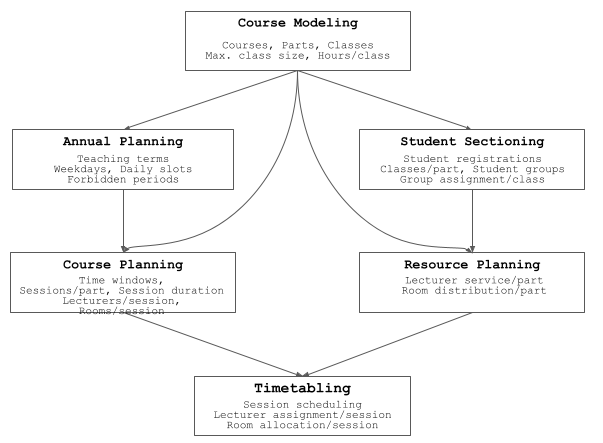
\includegraphics[scale=0.4]{img/utp_workflow.png}
\end{center}
\caption{Conventional workflow for course organization in French universities.}%: steps and roles}
\label{fig:utp-workflow}
\end{figure}

%The scope of these computational tasks and the overall workflow vary between countries and educational institutions as does the level of process automation and decision tool support \cite{2019oudevrielinkAOR}. 
Various problem formulations together with data formats and algorithms 
have been proposed in the literature to tackle specific aspects of university timetabling including 
curriculum balancing %for assigning courses to teaching termes while balancing student workload 
\cite{2001_castro_ARXIV,2012_chiarandini_JH,2013_rubio_MPE}, 
student sectioning \cite{2010_muller_AOR,2019_schindl_AOR}, 
%(strategic) room planning {2017lindhalEJOR}, 
examination timetabling \cite{1996_carter_JORS,2020_battistutta_CPAIOR,2010_mccollum_INFORMS},
curriculum-based %course timetabling \cite{2010mccollumINFORMS,2015bettinelliTOP},
or post-enrolment-based course timetabling \cite{2010_mccollum_INFORMS,2015_bettinelli_TOP,2007_lewis_ITC,2012_cambazard_AOR,2017_goh_EJOR,2021_chen_IEEEA},
tutor allocation \cite{2022_caselli_ESWA},
and minimal timetabling perturbation \cite{2019_lindahl_EJOR,2020_lemos_JS}.
Modeling languages have also been developed, notably the {\XML} language used in the 2019 international timetabling competition \cite{2018_muller_PATAT,2019_ITC} (which we refer to as the {\ITC} language)
which provides a catalog of constraints and supports model variability.
%We adopt a similar approach in this paper and introduce a domain-specific language ({\DSL}) modeling a broad class of university timetabling problems ({\UTP}). %that reduce to hard constraint satisfaction problems ({\CSP}). 
We adopt a similar approach in this paper and introduce a class of university timetabling problems called \UTP{} that involve course scheduling, resource allocation and student sectioning.
%We present a domain-specific language implemented in XML, called \XUTP{}, to encode \UTP{} instances.
%The {\UTP} language provides different features to tailor problem instances to each particular environment. It is designed around a formal domain model and a predicate language to state rules. Each instance is decomposed into a model of entities, a rule set and a solution component. Rules express collections of timetabling constraints on model entities and the solution component lists assignment decisions. Note that the solution may be void, partial or inconsistent. 
We present a domain-specific language to model \UTP{} instances (\UTP{} language) which %provides different features to tailor problem instances to each particular environment. It 
is designed around a formal domain model and a rules language to state constraints. Each instance is decomposed into a model of entities, a rule set and a solution component. Rules express collections of timetabling constraints on model entities and the solution component lists assignment decisions. The latter may be void, partial or inconsistent to accommodate different contexts (e.g., a solution for student sectioning to turn into a complete timetable, an outdated solution that must be revised or repaired). 

%Similarly to the schema proposed in \cite{2018muller,ITC2019} for the international timetabling competition ({\ITC}), 
Similarly to the {\ITC} language, 
the {\UTP} language adopts a multi-scale schedule horizon (i.e., weeks, weekdays and daily slots), a mixed set of resources (i.e., students, student groups, rooms and lecturers), and a hierarchical course structure (i.e., course parts, part classes and class sessions). In our approach however, class sessions (a.k.a., class meetings) are considered as first-class objects that must be scheduled individually alongside resources. 
The model supports single-resource sessions (e.g., single lecturer) as well as multi-resource sessions (e.g., hybrid teaching), and encodes core constraints relating to student sectioning, session scheduling and resource allocation. %which are cast using built-in properties and relations over entities (i.e., resources and course elements) and sessions. 
All resources are assumed cumulative (i.e., rooms, lecturers and students may host, teach and attend overlapping sessions) but this policy may be overridden with disjunctive scheduling rules.
The rules language effectively allows to enforce additional constraints on selected sets of sessions and entities (i.e., resources and course elements).
Rules are expressed using a catalog of timetabling predicates and a comprehension syntax to group, filter and bind sessions and entities. 
Specifically, each rule denotes a conjunction of \UTP{} constraints sharing the same predicate (e.g., periodicity of all lecture classes of a course) and constraints are technically generated through a rule flattening process. %on selected classes of entities and sessions 

%Specifically, the sessions of a course part are cast as single-resource (e.g., face-to-face lectures) or multi-resource sessions (e.g., hybrid sessions) by quantifying the needed resources. 
%Lecturers and rooms are distributed over course parts while students are distributed over courses based on registrations which determines the resources allowed for each session.
%%The resources allowed for a session follow from the distribution of student registrations over courses and that of lecturers and rooms over course parts. 
%The volume of sessions per student depends on individual course registrations as class attendance is compulsory; it is configurable per lecturer in each course part but is unconstrained for rooms. 
%%The volumes of sessions are configurable per teacher in each part (i.e., sessions quota) but pre-determined for students (i.e., class attendance is mandatory) and unconstrained for rooms. 
%No limits apply on simultaneous resource usage but for rooms whose hosting capacity must match class size. Any resource may hence be allocated to joint or overlapping sessions  (e.g., lecture and optional tutoring for students) except for rooms hosting multi-room sessions. In any case, rules may be enforced as needed to prevent sessions from overlapping or to make resources fully disjunctive. As for session scheduling, start time grids are configurable in each course part and the model simply requires full session sequencing in each class. Lastly, the model sections students into classes and supports subgroup inclusion constraints between classes. Note that student groups are considered a by-product of student sectioning and as such may only be listed in the solution component. 

%The rules language allows to state additional constraints using a catalog of timetabling predicates. A rule is tied to a predicate and models a conjunction of constraints on selected classes of entities and sessions (e.g., disjunctive scheduling rule for lecturers, temporal constraints on the courses of a curriculum). Each constraint applies to one or more pairs, called e-maps, and may involve parameters based on the predicate signature. An e-map either associates a resource with a subset of its compatible sessions or a course element with a subset of its constitutive sessions. In the first case, the e-map is interpreted as a set of conditional entity-to-session assignments while it is unconditional if it models a course element. Specifically, a constraint is only evaluated on the sessions for which its e-map argument(s) and the considered solution propose the same entity. Each predicate may be applied equally well to any type of e-map and be used to constrain resources (e.g., lecturer unavailability), course elements (e.g., class periodicity) or individual sessions (e.g., session parallelization). %Note that constraints on e-maps modeling sessions of course elements are de facto unconditional. 
%Formally, a rule is defined by a universally quantified formula wherein quantifiers restrict the domains of the e-map variables. A language of selectors is provided to build and filter domains of e-maps based on session ranks, entity identifiers, entity types, or any user-defined class of elements (e.g., team of lecturers, block of rooms). A rule hence denotes the conjunction of constraints obtained by instantiating the predicate over the cross-product of the domains of the e-map variables. 

\begin{figure}
    \centering
    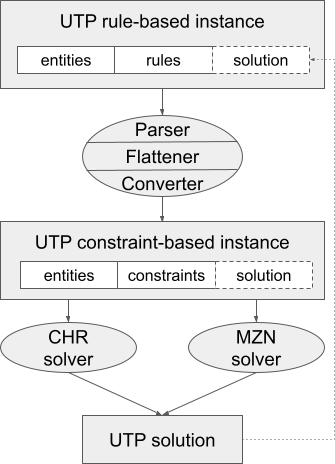
\includegraphics[scale=0.4]{img/utp_toolchain.png}
    \caption{The \UTP{} toolchain.}
    \label{fig:toolchain}
\end{figure}

Note that all constraints are handled as hard constraints and each {\UTP} instance is reduced to a hard constraint satisfaction problem ({\CSP}).
The ability to model preferences and multi-criteria objectives by the means of soft constraints is paramount in course timetabling and will be the subject of future extensions. 
Likewise, the catalog of {\UTP} predicates still lacks important constraints (e.g., gap, distribution and pattern constraints - see e.g. \cite{2017_aizam_AIPCP,2021_chen_IEEEA}) which will be gradually added in future versions.

As for implementation, the \UTP{} language is based on \XML{} and embedded in two constraint modeling languages, namely, 
{\MINIZINC} \cite{2007_nethercote_SPH,MINIZINC} and {\CHR} \cite{1994_fruhwirth_Chap}. 
We developed a tool chain consisting of a \XML{} parser, a rule processor to flatten rules into constraints, and an encoder to convert the resulting instances to solver-compatible formats %using {\JSON} or {\DZN}
(see Figure~\ref{fig:toolchain}). 
Beyond {\MINIZINC} and {\CHR}, constraint-based {\UTP} instances may be used as inputs to any solver implementing the model and predicates of the \UTP{} language.
We do not discuss here the \XML{} syntax of the language (the reader is referred to \cite{uspSite} which provides access to the detailed specification, %the {\JSON/\DZN} instance formats, 
%\cite{uspSite} also provides
the {\MINIZINC} and {\CHR} models, the tool suite, and a benchmark of instances).
Rather, we present the abstract syntax of the \UTP{} language and provide semantics for the key components.

The remainder of the paper is organized as follows.
Section~\ref{sec:schema} introduces the {\UTP} language and draws a comparison with %other modeling frameworks, notably 
the {\ITC} schema.
Section~\ref{sec:model} presents a generic constraint-based {\UTP} model.
Section~\ref{sec:cp-model} discusses its implementation using {\MINIZINC} and {\CHR}
and the cross-validation of the models on a real instance. 
Section~\ref{sec:conclusion} concludes and discusses extensions of this work.
%------------------------------------------------------------
%------------------------------------------------------------
\section{University Timetabling Problem}
\label{sec:schema}
A \UTP{} instance is defined by an entity model and a rules set. %and a solution. % and a pre-assignment. 
%The entity model defines the schedule horizon, courses and resources of the instance and encodes core constraints relating to session scheduling, resource allocation, and student sectioning.
%Rules express additional constraints meant to capture stakeholder requirements on particular aspects of the problem.
%A rule is a conjunction of constraints built from a catalog of timetabling-specific predicates.
%The solution is a list of choices made for some or all of the decisions at stake (e.g., start time of a session).
%Note that a \UTP{} instance may have no rules.% rules set and solution components may be omitted. 
% Besides, the listed solution is not required to be consistent with the constraints enforced by the entity model or the rules set.
% This allows to tackle subproblems using separate instances and to support timetable generation or repair tasks.
% Each rule is an intensional representation of a collection of constraints applying to different entities.
% {\UTP} instances may thus be compiled to lower-level representations that explicitly declare all constraints and whose format is compatible with {\CP} languages.
%{\UTP} instances may therefore be compiled into lower-level representations that lists all constraints and whose format is tailored to back-end solvers.
%
A solution to a \UTP{} instance is a list of choices made for all the decisions at stake %(e.g., start time of a session).
that satisfies the core constraints of the entity model and the constraints expressed by the rules.
%Note that a \UTP{} instance may have no rules and an input solution may be provided based on context.
%We defined \acronym{XUTP}, an embedded version of the \UTP{} language into \XML{}.
%We do not provide here the detailed \XML{} specification of \acronym{XUTP} (see~\cite{uspSite}).
We provide in this section an informal description and set-theoretic semantics for the \UTP{} language components, namely the entity model (Section~\ref{sec:entity-model}), constraints (Section~\ref{sec:constraints}), rules (Section~\ref{sec:rules}) and solution (Section~\ref{sec:solution}).
Section~\ref{sec:related-work} draws a comparison between the \UTP{} language and the \ITC{} schema.


%
%We present theses components in turn, 
%discuss the type of features and requirements that may be factored in,
%and provide set-theoretic semantics for the rules language and flattening process.
%The reader is referred to \cite{uspSite} for the detailed {\XML} specification of {\XUTP} and the {\JSON/\DZN} instance formats.
%\cite{uspSite} also provides access to the {\MINIZINC} and {\CHR} models, the tool suite, and a benchmark of instances.
%motivate design choices,
%whose {\CP} implementation is addressed in Section~\ref{sec:model}.

%motivate design choices, 
%and highlight differences with related work.

%------------------------------------------------------------
%------------------------------------------------------------
\subsection{Entity model}
\label{sec:entity-model}
The entity model of a {\UTP} instance defines its schedule horizon, course structure and resources, as well as properties of entities and relational maps (see 
Figure~\ref{fig:utp-entity-model} for a sketch of the meta-model and Figure~\ref{fig:utp-rule-1} for a toy example).  
First, the entity model uses a time grid that decomposes into weeks, weekdays and daily slots. %, the number of which is instance-specific. 
Weeks share the same weekdays and weekdays the same daily slots. The latter make up 24 hours and have the same duration. %measured in minutes. 
Note that neither successive weeks nor successive weekdays are assumed to be consecutive. %and that Monday is the first weekday by convention. 
The schedule horizon is implicitly defined by the series of time slots mapping to week, weekday and daily slot combinations. Slots hence serve as time points to represent start and end times of course sessions and to measure session duration, travel time and any gap between sessions.

% % For one-column wide figures use
% \begin{figure}[h]
% % \includegraphics{utp-time-grid.eps}
% \caption{{\UTP} 3-layered time grid}
% \label{fig:utp-time-grid}
% \end{figure}

Courses have a tree-structure wherein each course (e.g., Algorithms) decomposes into parts (e.g., Lecture and Lab), parts into classes (e.g., lecture classes A and B), and classes into sessions (e.g., sessions 1 to 10 for each lecture class). Class sessions are the elementary tasks to schedule when solving a {\UTP} instance and the model fixes their number, duration and sequencing. First, the classes of a course part are decomposed into an identical number of sessions of equal duration, both constants being part-specific. Although this approach forbids classes using different session durations in a course part, 
%it %provides flexibility for handling sessions independently wrt. scheduling and resource allocation.
%Fixed decompositions also 
it is paramount to capture requirements that rely on clear-cut sessions (e.g., starting lab classes after 2 lecture sessions, synchronizing the 5th sessions of the lab classes for a joint examination). Second, the sessions of a class are ranked in the model and must be sequenced accordingly in any solution (session 1 before session 2 \ldots). Note that sessions are considered uninterruptible and, in particular, may not overlap two days. 

\begin{figure}[ht]
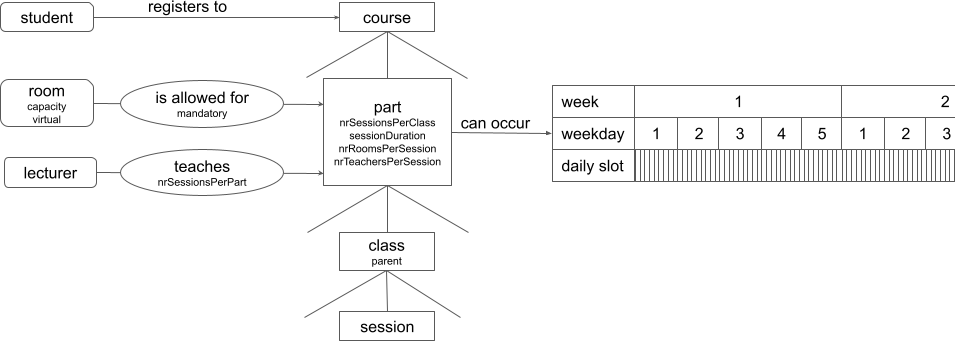
\includegraphics[scale=0.35]{img/utp_entity_model.png}
\caption{Entity meta-model.}
\label{fig:utp-entity-model}
\end{figure}

{\UTP} resources fall into 4 types, namely, rooms, lecturers, students and (student) groups.
All the resources of an instance, except groups (see Section~\ref{sec:solution}), are declared and typed in the entity model. In practice, upstream processes and decisions %constrain the resourcing and timing of courses.
%Basic restrictions come in the form of compatibility constraints that list 
determine the suitable rooms, eligible lecturers, candidate students and allowed times for the different courses (e.g., faculties prescribing degree-specific time grids, departments implementing room pooling policies and naming lecturers for courses, students registering to courses). %Such constraints are built in the entity model but scoped differently depending on resource types. %Specifically, 
These compatibility constraints are modeled by associating sets of possible start times, rooms and lecturers to each course part and a set of registered students to each course. Each session then inherits the sets of allowed resources from the course part and the course it belongs to.
%and which are implicitly the sessions.
%Student registrations are listed separately and %the possible students for a session are those registered to the course it sits in.
%any student registered to a course is considered a possible candidate for each of its sessions.

The entity model also encodes flow constraints that govern the distribution of resources over courses based on student registrations and capacity planning decisions (e.g., workload distribution between lecturers). First, each lecturer is allocated a fixed number of sessions in each course part he is eligible for, leaving lecturer-to-session assignment decisions to solvers. Second, each room allowed in a course part may be freely allocated to any session of the part (possibly none) but the model provides the flexibility to mark a room as mandatory in which case it will host or co-host all the sessions. As for students, the sectioning policy is implicit and complies with the course structure, i.e., each student must be assigned to a single class in each part of a course he has registered to and attend all sessions of these classes. In addition, the model supports group nesting constraints between classes to implement course-specific policies (e.g., aggregating student groups bottom-up from labs to lectures) or cross-course sectioning (e.g., imposing the same groups between classes of different courses of a curriculum).
 
Resource utilization is naturally subject to demand and capacity constraints.
Since modalities differ from one environment to the next, the language supports disjunctive and cumulative resources. The default policy is to consider all students, groups, lecturers and rooms as cumulative resources, i.e., they can attend, teach or host simultaneous sessions. Note though that rules may be stated to make some resources fully disjunctive or to prevent specific sessions from overlapping. Support for cumulative resources is paramount to address flexible attendance requirements (e.g., students assigned optional tutoring sessions that may overlap with compulsory courses) or to handle multi-class events (e.g., rooms hosting several classes for an exam or a conference). The model imposes no limits on the number of parallel sessions lecturers and students may attend. Rooms however may only host class sessions whose cumulated headcount is within their capacity. Upper bounds on room capacity and class size are encoded for all rooms and classes and the model also allows uncapacitated rooms to cater for the case of virtual rooms.

The language also supports sessions using multiple resources of the same type. %at any point in time.
The need for multiple rooms or lecturers arises in practical situations (e.g., multi-room sessions for hybrid teaching, joint supervision of practical work sessions, exams requiring several monitors). %and the number of resources required per session is course part dependent.
%such restrictions are expressed in the entity model through cardinality constraints. %that are lifted to course parts. 
To this end, the model associates to each course part the number of lecturers required per session 
and indicates whether the sessions are single- or multi-rooms.
Note that sessions without lecturers or rooms are allowed (e.g., unsupervised student project sessions).
The model enforces specific constraints to handle multi-room sessions which override the default room allocation policy. Specifically, students attending the session may be freely dispatched in rooms irrespectively of the group structure, the cumulated capacity of the allocated rooms is taken into account for hosting, uncapacitated rooms cannot be allocated, and 
the allocated rooms are considered disjunctive for the time of the session.
%a {\UTP} instance may freely mix single- and multi-resource sessions as well as disjunctive and cumulative resources. 

Note finally that the language provides users with the ability to label resources and course elements to define their own classes of entities (e.g., teams of lecturers, blocks of rooms). Labels together with built-in entity types and identifiers are used to filter entities and to scope rules appropriately.
 


We formalize below the entity model and introduce notations that will be used thereafter.
Let ${\ENTITY}$ denote the set of entities
and ${\SESSION}$ the set of sessions.
${\ENTITY}$ is partitioned into   
a set of courses ${\COURSE}$, 
a set of course parts ${\PART}$, 
a set of classes ${\CLASS}$, 
a set of students ${\STUDENT}$, 
a set of lecturers ${\TEACHER}$,
a set of rooms ${\ROOM}$,
and the singleton domain of courses ${\COURSES}$ 
(${\COURSES}=\myset{\COURSE}$). 
Let 
%${\COURSES}$ denote the course domain, 
%${\COURSE}$ the set of courses (${\COURSES}=\myset{\COURSE}$), 
%${\PART}$ the set of course parts, 
%${\CLASS}$ the set of classes, 
%${\SESSION}$ the set of sessions, 
%${\STUDENT}$ the set of students, 
%${\TEACHER}$ the set of teachers, 
%and 
%${\ROOM}$ the set of rooms.
$
{\TYPE}
=
\myset{
{\COURSES}, 
{\COURSE},
{\PART},
{\CLASS},
{\STUDENT},
{\TEACHER},
{\ROOM}
}
$
denote the set of entity types
(${\ENTITY}=\setunion{X}{\TYPE}{X}$)
and 
$
{\prec}
=
\myset{
({\COURSES},{\COURSE}),
({\COURSE},{\PART}),
({\PART},{\CLASS}),
({\CLASS},{\SESSION}),
({\STUDENT},{\COURSE}),
$
$
({\TEACHER},{\PART}),
({\ROOM},{\PART})
}
$
denote the relation over 
${\TYPE}\cup\myset{\SESSION}$ 
that models the course hierarchy
and the distribution of resource types over course components.

${\prec^{*}}$
%${\preceq^{*}}$
denotes the transitive %and reflexive 
closure of
${\prec}$ 
over
${\TYPE}\cup\myset{\SESSION}$
and
${\maptype{X}{Y}}:X\rightarrow2^{Y}$
denotes the function mapping each element of $X$ to its set of compatible elements in $Y$
for each pair %$(X,Y)$ such that 
%$X{\preceq^{*}}Y$.
$X{\prec^{*}}Y$.
For instance, 
${\maptype{\ROOM}{\PART}}$ 
represents the distribution of rooms over course parts, 
${\maptype{\PART}{\CLASS}}$ 
the decomposition of course parts into classes,
${\maptype{\CLASS}{\SESSION}}$ 
the decomposition of classes into sessions,
and ${\maptype{\ROOM}{\SESSION}}$ 
the inferred distribution of rooms over sessions.
The functions corresponding to the pairs of $\prec$
are directly encoded in the entity model
and the remaining functions are defined inductively using recursive aggregation. 

We shall denote by ${\map{X}{Y}{i}}$ the image of entity $i$ of type $X$ over $2^Y$ %, i.e., the set of elements of type $Y$ compatible with $i$. 
and by ${\maptype{Y}{X}}$ the inverse of ${\maptype{X}{Y}}$.
Equation (\ref{model:hierarchy}) below models the hierarchical decomposition of course elements\footnote{$\sqcup$ denotes the disjoint union operation, i.e. set union over pairwise disjoint sets.},
Equation (\ref{model:transitivity}) is the closure rule over 
%$\preceq^{*}$. 
$\prec^{*}$,
%Note that each map $\maptype{\SESSION}{X}$ is the inverse of map $\maptype{X}{\SESSION}$.
and Equation (\ref{model:inverse}) models inverse maps.

\begin{align}
%
\forall (X,Y) \in 
\myset{
({\COURSES},{\COURSE}),
({\COURSE},{\PART}),
({\PART},{\CLASS}),
({\CLASS},{\SESSION})
}:
Y=
\setpartition{i}{X}{\map{X}{Y}{i}} 
\label{model:hierarchy}
\\
%
\forall X,Y,Z \in {\TYPE}\cup\myset{\SESSION}:
X\preceq^{*} Y\preceq^{*} Z 
\Rightarrow 
(\forall i \in X:
\map{X}{Z}{i}=\setpartition{j}{\map{X}{Y}{i}}{\map{Y}{Z}{j}}
\label{model:transitivity})
\\
%
\forall X,Y \in {\TYPE}:
X\preceq^{*} Y 
\Rightarrow 
(\forall i \in X, j \in Y:
j \in \map{X}{Y}{i} \Leftrightarrow i \in \map{Y}{X}{j}
)
\label{model:inverse}
%\\
%%
%\forall X \in {\TYPE}\cup\myset{\SESSION},
%i \in X:
%\domarg{X}{X}{i} = \myset{i} \label{model:selfmap}
%%
\end{align}



\begin{table}[ht]
\begin{center}
\begin{tabular}{|rl|}
\hline
$(\WEEK,\WEEKDAY,\DAILYSLOT)$               & the number of weeks $\WEEK$, weekdays $\WEEKDAY$ and daily slots $\DAILYSLOT$
\\
$\SLOT$                                     & the time slots 
\\\hline
$\ENTITY$                                   & the entities
\\
$\COURSES\subseteq\ENTITY$                  & the course domain
\\
$\COURSE\subseteq\ENTITY$                   & the courses
\\
$\PART\subseteq\ENTITY$                     & the course parts
\\
$\CLASS\subseteq\ENTITY$                    & the classes
\\
$\ROOM\subseteq\ENTITY$                     & the rooms
\\
$\TEACHER\subseteq\ENTITY$                  & the lecturers
\\
$\STUDENT\subseteq\ENTITY$                  & the students
\\
$\map{X}{Y}{i}\subseteq{Y}$                 & the entities of type $Y$ associated with entity $i$ of type $X$
\\\hline
${\LABEL}\subseteq2^{{\ENTITY}}$            & the labels
\\\hline
$\GROUP\subseteq{2^{\STUDENT}}$             & the groups of students
\\\hline
$\SESSION$                                  & the sessions
\\
$\map{X}{\SESSION}{i}\subseteq{\SESSION}$   & the sessions compatible with entity $i$ of type $X$
\\
$\map{\SESSION}{X}{s}\subseteq{X}$          & the entities of type $X$ compatible with session $s$
%\\
%$\disjunctiverooms\subseteq{\ROOM}$         & the set of disjunctive rooms
\\
$\partallowedslots{s}\subseteq{\SLOT}$      & the start times allowed for session $s$
\\
$\sessionduration{s}\in{\SLOT}$             & the duration of session $s$
\\
$\sessionrank{s}\in{\NATURAL^*}$            & the rank of session $s$ in its class
\\
$\sessionranked\subseteq{\SESSION\times\SESSION}$ & the pairs of sessions with consecutive ranks in a class
\\\hline
$\classparents{k}\subseteq{\CLASS}$          & the parent classes of class $k$ if any
\\
$\classcapacity{k}\in{\NATURAL}$            & the maximum size of class $k$
\\\hline
$\roomcapacity{r}\in{\NATURAL}$             & the capacity of room $r$
\\
$\virtualroom{r}\in{\BOOLEAN}$              & whether room $r$ is virtual or not
\\
$\virtualrooms\subseteq{\ROOM}$             & the virtual rooms
\\\hline
$\multiroompart{p}\in{\BOOLEAN}$            & whether course part $p$ is multi-room or not
\\
$\multiroomparts\subseteq{\PART}$           & the multi-room parts
\\
$\mandatoryrooms{p}\subseteq{\ROOM}$        & the mandatory rooms of part $p$
\\
$\partteachermultiplicity{p}\in{\NATURAL}$  & the number of lecturers required by every session of part $p$
\\
$\partteacherservice{l,p}\in{\NATURAL}$     & the number of sessions required by lecturer $l$ in part $p$
\\
\hline
\end{tabular}
\caption{Entity model: constants, sets, maps and relations.}
\label{table:model-maps}
\end{center}
\end{table}


Table~\ref{table:model-maps} provides the full list of constants, sets, properties and relational maps encoded in the entity model.\footnote{
The following rules apply. $\SLOT=\myset{i.\WEEKDAY.\DAILYSLOT+j.\DAILYSLOT+k\ |\ 0\leq i<\WEEK,0\leq j<\WEEKDAY,1\leq k\leq\DAILYSLOT}$.
For each class $k$ in part $p$,
$\myset{\sessionrank{s}\ |\ s\in\map{\CLASS}{\SESSION}{k}}=\myset{1,\ldots,\mycard{\map{\CLASS}{\SESSION}{k}}}$, 
%$\mycard{\classparents{k}}\leq1$ 
and $\classparents{k}\not\subset\map{\PART}{\CLASS}{p}$.
For each pair of sessions $s,s'$, 
$(s,s')\in\sessionranked$ iff $\map{\SESSION}{\CLASS}{s}=\map{\SESSION}{\CLASS}{s'}$ and $\sessionrank{s'}=\sessionrank{s}+1$.
For each course part $p$,
%$p\in\multiroomparts$ iff $\multiroompart{p}$; 
%and 
$\partteachermultiplicity{p}.\mycard{\map{\PART}{\SESSION}{p}}=\sum\limits_{l\in\map{\PART}{\TEACHER}{p}}{\partteacherservice{l,p}}$.}

%We shall denote by
%${\RANK}$
%the range of session ranks,
%${\maptype{\RANK}{\SESSION}}:\RANK\rightarrow2{^\SESSION}$
%the rank-based partitioning of sessions,
%and
%${\LABEL}$
%the set of labels 
%(${\LABEL}\subseteq2^{{\ENTITY}}$)
%completed 
%with the whole set of entities %to mock label optionality
%($\ENTITY\in{\LABEL}$)
%and singleton entities %to support identity-based selection
%($\myset{\myset{e}\ |\ e\in{\ENTITY}}\subseteq{\LABEL}$).
%As discussed in section~\ref{sec:rules},
%labels are optional filters used in rules to select entities
%hence the formal inclusion of $\ENTITY$ in ${\LABEL}$ to mock label optionality.
%Likewise, entity identifiers are used as an alternative to labels
%hence the inclusion of singleton entities in ${\LABEL}$.

%------------------------------------------------------------
%------------------------------------------------------------
\subsection{Predicates and constraints}
\label{sec:constraints}
{\UTP} constraints apply to pairs, called e-maps, which associate an entity with a non-empty subset of its compatible sessions.
%which we call e-maps. 
Constraints are built with predicates whose signature includes e-map variables%ranging over the set of e-maps
, the number of which is referred to as the arity of the predicate. 
Note that some predicates may also accept parameters.
Let 
${\EMAP}=
\setunion{X}{\TYPE}
\myset{(e,S')\ |\ e\in X,S'\subseteq\map{X}{\SESSION}{e}\wedge S'\neq\emptyset}$
denote the set of e-maps,
a {\UTP} constraint has the form
\begin{align}
c((e_1,S_1),\ldots,(e_m,S_m),p_1,\ldots,p_n) \label{rule:constraint}
\end{align}
where 
$c$ is a predicate symbol of arity $m$,
$(e_1,S_1),\ldots,(e_m,S_m)$ are e-maps ($(e_i,S_i)\in{\EMAP}$, $i=1\ldots m$) 
and 
$p_1,\ldots,p_n$ are values for the parameters of $c$ ($n\geq0$).
Three constraints (\ref{constraint-example-1}, \ref{constraint-example-2}, \ref{constraint-example-3}) are illustrated in Figure~\ref{fig:utp-rule-1}.


Every predicate may be used indistinctly with e-maps defined on course elements or on resources.
E-maps defined on resources are interpreted as conditional session-to-resource assignments
when checking constraints 
whereas e-maps defined on course elements are unconditional assignments since they model constitutive sessions.
In other words, 
a constraint is only evaluated
on the sessions for which its e-map arguments and the considered solution propose the same entity assignment.\footnote{Formally, let $\var{E}{\SESSION}{e}$ be the variable denoting the set of sessions assigned to entity $e$ and $S'_1,\ldots,S'_m$ be sets of sessions, the conditionality of a constraint $c$ is stated as follows: 
$(\var{E}{\SESSION}{e_1}=S'_1 \wedge\ldots\wedge\var{E}{\SESSION}{e_m}=S'_m)
\Rightarrow
(c((e_1,S_1),\ldots,(e_m,S_m),p_1,\ldots,p_n)
\Leftrightarrow
c((e_1,S_1\cap S'_1),\ldots,(e_m,S_m\cap S'_m),p_1,\ldots,p_n))$.}

It follows that 
a constraint is evaluated on every session that is mapped to a course element by one of its e-map arguments.
Constraints that apply exclusively to course elements are therefore unconditional. 
Note also that the use of e-maps that model the whole set of sessions compatible with an entity 
will necessarily constrain any session that may be assigned to this entity.


%Every predicate may be used indistinctly with e-maps defined on course elements or on resources which we call c-maps and r-maps, respectively. R-maps are interpreted conditionally since they map a resource to some of its possible sessions whereas c-maps model unconditional assignments since they model constitutive sessions of course elements. In other words, a constraint must be evaluated on every session of every c-map in its scope but only on the sessions of its r-maps whose resource assignment is compatible with the proposed solution.\footnote{Formally, let $\var{E}{\SESSION}{e}$ be the variable denoting the set of sessions assigned to entity $e$ and $S'_1,\ldots,S'_m$ be sets of sessions, the conditionality of a constraint $c$ is stated as follows:  $(\var{E}{\SESSION}{e_1}=S'_1 \wedge \var{E}{\SESSION}{e_m}=S'_m) \Rightarrow (c((e_1,S_1),\ldots,(e_m,S_m),p_1,\ldots,p_n) \Leftrightarrow c((e_1,S_1\cap S'_1),\ldots,(e_m,S_m\cap S'_m),p_1,\ldots,p_n))$.}
%effectively assigns to the resource of the r-map.
%(see Rule (\ref{rule:conditionality})).
%It follows that constraints applying exclusively to c-maps are unconditional. Besides, the scoping of e-maps that model the whole set of sessions compatible with an entity will constrain every session assigned to a resource or constitutive of a course element.
%%The rule below %(\ref{rule:conditionality}) models the conditionality of constraints.

%{\footnotesize{
%\begin{multline}
%\forall S'_1,\ldots,S'_m\in{\SESSION}:
%(\var{E}{\SESSION}{e_1}=S'_1 \wedge \var{E}{\SESSION}{e_m}=S'_m)
%\Rightarrow\\
%(c((e_1,S_1),\ldots,(e_m,S_m),p_1,\ldots,p_n)
%\Leftrightarrow
%c((e_1,S_1\cap S'_1),\ldots,(e_m,S_m\cap S'_m),p_1,\ldots,p_n))
%\label{rule:conditionality}
%\end{multline}
%}}

\begin{table}[ht]
\resizebox{\textwidth}{!}{%
\centering
\begin{tabular}{|l|l|l|l|}
\hline
\textbf{Name}               & \textbf{Arity} & \textbf{Parametric} & \textbf{Semantics}\\ \hline

%assign\_slot               & 1         & yes   & Assign a slot or slot tuple to a session\\ \hline
%assign\_room               & 1         & yes   & Assign a set of room to session in entry\\ \hline

%allocation\_group           & 1        & no    & Domain allocation for class with group in the solution\\ \hline
%part\_schedule              & 1        & no    & Allowed start time slots for sessions\\ \hline
%domain\_class\_group        & 1        & no    & Allowed groups for classes (solution input)\\ \hline
%domain\_session\_teacher    & 1        & no    & Allowed teachers for sessions\\ \hline
%domain\_class\_room         & 1        & no    & Allowed rooms for sessions\\ \hline

{\SAMEDAILYSLOT}            & 1         & no    & Sessions start on the same daily slot\\ \hline
{\SAMEWEEKDAY}              & 1         & no    & Sessions start on the same weekday\\ \hline
{\SAMEWEEKLYSLOT}           & 1         & no    & Sessions start on the same weekly slot\\ \hline
{\SAMEWEEK}                 & 1         & no    & Sessions start the same week\\ \hline
{\SAMEDAY}                  & 1         & no    & Sessions start the same day\\ \hline
{\SAMESLOT}                 & 1         & no    & Sessions start at the same time\\ \hline
{\FORBIDDENPERIOD}          & 1         & yes   & Sessions cannot start in the given time period\\ \hline
{\ATMOSTDAILY}              & 1         & yes   & The number of sessions scheduled in the daily period is upper-bounded\\ \hline
{\ATMOSTWEEKLY}             & 1         & yes   & The number of sessions scheduled in the weekly period is upper-bounded\\ \hline
%implicit\_sequenced\_sessions & 1 & \multicolumn{4}{|c|}{no} & All sessions in classes are sequenced\\ \hline
{\SEQUENCED}                & $\geq2$   & no    & Sessions are sequenced\\ \hline
{\WEEKLY}                   & 1         & no    & Sessions are weekly \\ \hline

{\NOOVERLAP}                & 1         & no    & Sessions cannot overlap\\ \hline
{\TRAVEL}                   & 1         & yes   & Travel time is factored in if sessions hosted in the given rooms\\ \hline

{\SAMEROOMS}                & 1         & no    & Sessions are hosted in the same room(s)\\ \hline
{\SAMESTUDENTS}             & 1         & no    & Sessions are attended by the same student(s)\\ \hline
{\SAMETEACHERS}             & 1         & no    & Sessions are taught by the same lecturer(s)\\ \hline

{\ADJACENTROOMS}            & 1         & yes   & Sessions are hosted in the given adjacent rooms\\ \hline

{\TEACHERDISTRIBUTION}      & $\geq2$   & yes   & Distributes lecturer workload over classes\\ \hline

\end{tabular}
}
\caption{Catalog of {\UTP} predicates.}
\label{tab:predicate_catalog}
\end{table}


% 
% \newcolumntype{M}[1]{>{\raggedright}m{#1}}
%\begin{table}[!h]
%    \centering
%    \begin{tabular}{|l|M{2cm}|*{7}{c|}}
%        \hline
%        \multirow{2}{4em}{Name} & \multirow{2}{4em}{Entity} & \multirow{2}{1cm}{Arity} & \multicolumn{4}{|c|}{Parameter} & \multirow{2}{6em}{Conditional} & \multirow{2}{10em}{Explication}   \\
%        \cline{4-7}
%           & & &name& type& number& type & &    \\
%        \hline
%
%
%assign\_slot & All & max 1 & slot & max 1 & min 1 & slots  & yes & Assign a slot or slot tuple to a session\\ \hline
%
%allocation\_group&Part& max 1  & \multicolumn{4}{|c|}{no}  & no  & Domain allocation for class with group in the solution\\ \hline
%
%assign\_room  & Course, Part, Class, Sessions, Teacher, Student &max 1 &rooms &  1 & min 1 &room & yes & Assign a set of room to session in entry\\ \hline
%
%\multirow{2}{6.5em}{at\_most\_daily} & \multirow{2}{2cm}{Course, Part, Class, Teacher, Room, Student }& \multirow{2}{4em}{max 1} &count & 1 & 1 & slot &\multirow{2}{4em}{ yes} &\multirow{2}{4em}{ Limit a number of session in intervalle } \\ 
%\cline{4-7}
%  & & &first& 1& 1& slot & &    \\
%  \cline{4-7}
%  & & &last& 1& 1& slot & &    \\
%\hline
%at\_most\_weekly & Course, Part, Class, Teacher, Room, Student & max 1 & count &  1 & 1 & slot & yes & Limit a number of session in intervalle \\ \hline
%
%connected\_room &  Course, Part, Class, Teacher, Room, Student & max 1 & roomChain & min 1  & min 2 & room [ordered]  & yes & Session need connected rooms \\ \hline
%
%disjunctive\_group & Student & max 1 & \multicolumn{4}{|c|}{no} & yes & A group cant have overlap of 2 sessions  \\ \hline
%
%disjunctive\_room & Room   & max 1 & \multicolumn{4}{|c|}{no} & yes & A room cant host 2 sessions at same moment  \\ \hline
%
%disjunctive\_teacher & Teacher & max 1 & \multicolumn{4}{|c|}{no} & yes & A teacher cant gives  classes at same moment\\ \hline
%
%domain\_class\_group & Class & max 1 & \multicolumn{4}{|c|}{no} & no & A subset of group to classes (need solution)\\ \hline
%
%domain\_session\_teacher & Session & max 1 & \multicolumn{4}{|c|}{no} & no & A subset of teacher for sessions\\ \hline
%
%domain\_class\_room &Class & max 1 & \multicolumn{4}{|c|}{no} & no & A subset of room for class \\ \hline
%
%\multirow{2}{5.5em}{forbidden\_slot} & \multirow{2}{4em}{All} & \multirow{2}{4em}{max 1} & first & 1 & 1& slot & \multirow{2}{4em}{yes} & \multirow{2}{4em}{A session cant take slot in intervalle} \\
%  \cline{4-7}
%  & & &last& 1& 1& slot & &    \\
%\hline
%
%implicite\_sequenced\_sessions & Class & max 1 & \multicolumn{4}{|c|}{no} & no & All sessions in classes are sequenced\\ \hline
%
%\multirow{2}{9em}{not\_consecutive\_rooms} &\multirow{2}{2cm}{ Course, Part, Class, Teacher, Student} &\multirow{2}{4em}{ max 1} & minGap & 1 & 1 & slot & \multirow{2}{4em}{yes} & \multirow{2}{4em}{If 2 sessions have rooms in tuple then need a gap of mingap to walk from one the other} \\ 
%  \cline{4-7}
%  & & &rooms& 2 & min 1 & room,label & &   \\
%\hline
%
%part\_schedule & all & max 1 & \multicolumn{4}{|c|}{no}  & yes & we allowed time part value\\ \hline
%
%same\_daily\_slot & all & min 1 & \multicolumn{4}{|c|}{no} & yes & all slots of  selected sessions  are equal to the same daily slot \\ \hline
%
%same\_day  & all & min 1 & \multicolumn{4}{|c|}{no} & yes & all slots of  selected sessions  are equal to the same day \\ \hline
%
%same\_rooms & Course, Part, Class, Session, Teacher, Student  & min 1 & \multicolumn{4}{|c|}{no} & yes & all set rooms of  selected sessions  are equal \\ \hline
%
%same\_slots & all  & min 1 & \multicolumn{4}{|c|}{no} & yes & all slots of  selected sessions  are equal \\ \hline
%
%same\_teachers & Course, Part, Class, Session, Room, Student  & min 1 & \multicolumn{4}{|c|}{no} & yes & all set teachers of  selected sessions  are equal \\ \hline
%
%same\_week & all & min 1& \multicolumn{4}{|c|}{no} & yes & all slots of  selected sessions  are equal to the same week \\ \hline
%
%same\_weeklyday & all & min 1 & \multicolumn{4}{|c|}{no} & yes & all slots of  selected sessions  are equal to the same weekly day \\ \hline
%
%same\_weeklyslot & all & min 1 & \multicolumn{4}{|c|}{no} & yes & all slots of  selected sessions  are equal to the same weekly slot \\ \hline
%
%sequenced & Course, Part, Class, Session & min 1 & \multicolumn{4}{|c|}{no} & no & Sessions are ordered in the horizon slot (i.e i < j slot[session[i]] < slot[session[j]] \\ \hline
%
%teacher\_repartition & Class & min 2& class & min 2 & 1 & option  & no & repartition of teacher into a differentes classes of part \\ \hline
%
%weekly & Course, Part, Class, Session & min 1& \multicolumn{4}{|c|}{no} & no & A session tuple is weekly \\ \hline
%    \end{tabular}
%    \caption{Catalog of {\UTP} predicates}
%    \label{tab:catalog_constraint}
%\end{table}

Table \ref{tab:predicate_catalog} lists the predicates of the language
and indicates which are variadic or parametric.
The first predicates 
\texttt{\SAMEDAILYSLOT},
\ldots,
%\texttt{\SAMEWEEKDAY},
%\texttt{\SAMEWEEKLYSLOT},
%\texttt{\SAMEWEEK},
%\texttt{\SAMEDAY} and
\texttt{\SAMESLOT}
enforce common restrictions on the start times of the targeted sessions (e.g., sessions starting the same day).
Additionally,
any start time interval may be forbidden 
by passing its start and end points 
as parameters to 
predicate \texttt{\FORBIDDENPERIOD}.
Predicates \texttt{\ATMOSTDAILY}
and
\texttt{\ATMOSTWEEKLY}
upper-bound
the number of sessions
scheduled daily or weekly
within the given time interval.
\texttt{\SEQUENCED}
is a n-ary predicate ($n\geq2$)
which constrains
the latest session of the $i$-th e-map 
to end before
the earliest session of $i+1$-th e-map ($i=1..n-1$).
Predicate 
\texttt{\WEEKLY}
ensures sessions
are scheduled weekly
without presuming any particular sequencing.
Predicate
\texttt{\NOOVERLAP}
ensures sessions do not overlap in time
and is typically used to model disjunctive resources.
Predicate \texttt{\TRAVEL}
factors in any travel time
incurred between consecutive sessions
hosted in distant rooms.
The travel time matrix is a parameter of the predicate.
\texttt{\SAMEROOMS},
\texttt{\SAMESTUDENTS}
and
\texttt{\SAMETEACHERS}
require that sessions be assigned to the same set of rooms,
students or lecturers.
Predicate 
\texttt{\ADJACENTROOMS}
require that sessions be hosted in 
adjacent rooms 
based on an adjacency graph passed as a parameter.
Lastly, 
predicate \texttt{\TEACHERDISTRIBUTION}
distributes the volumes of sessions represented by the different e-map arguments 
among different lecturers. Lecturers and session volumes are parameters of the predicate.


%------------------------------------------------------------
%------------------------------------------------------------
\subsection{Rules}
\label{sec:rules}
%For instance, unconditional start time restrictions using predicates such as {\SAMEDAILYSLOT} or {\FORBIDDENPERIOD}  may be enforced on any set of sessions bound to a course, a part, a class or more generally to the course domain. Conversely, start time restrictions on a set of sessions bound to a resource will only be enforced on those which are eventually assigned to the resource.
%Predicates serve to constrain the possible sessions of resources (e.g., unavailabilities of a teacher) or the constitutive sessions of course elements (e.g., periodicity of a class). 
%e-maps may then be adjusted to constrain candidate sessions of resources (e.g., teacher unavailability), constitutive sessions of course elements (e.g., class periodicity), or individual sessions (e.g., session sequencing and parallelization).
Rules are used to state conjunctions of constraints and in particular single constraints. %and in particular individual (singleton) constraints.
Each rule is defined by a universally quantified formula which bounds the domains of the e-map variables of a given predicate.
The collection of constraints hence represented is derived by instantiating the predicate with each tuple of e-maps belonging to the cross-product of the prescribed domains.
E-map domains are not given in extension
but represented using a language of selectors
%which provides a comprehension syntax 
allowing to generate and filter e-maps.
Let 
${\SELECTOR}$
denote the language of e-map domain selectors,
%(${\SELECTOR}\subseteq({\TYPE}\times{\LABEL}\times{2^{\RANK}})^{n}$).
a {\UTP} rule has the form %is a tuple 
\begin{align}
c(F_1,\ldots,F_m,p_1,\ldots,p_n)
\end{align}
and is interpreted by %The semantics of a rule $(c,D_1,\ldots,D_m,p_1,\ldots,p_n)$ is 
the %quantified 
formula
\begin{flalign}
&\forall (e_1,S_1)\in\denote{F_1},\ldots,(e_m,S_m)\in\denote{F_{m}}:
c((e_1,S_1),\ldots,(e_m,S_m),p_1,\ldots,p_n)
&\label{rule:rule}
\end{flalign}
where 
$c$ is a predicate symbol of arity $m$,
$F_1,\ldots,F_m$ are selectors ($F_i\in{\SELECTOR}$, $i=1\ldots m$),
$\denote{F_i}$
denotes the domain of e-maps represented by
selector 
$
F_i\in{\SELECTOR}
$,
and
$p_1,\ldots p_n$ are values for the parameters of $c$ ($n\geq0$),
.

The language of selectors allows 
to target entities based on type, label or identifier
and
to filter their sets of sessions
based on session rank and mutual compatibility with other entities.
It is complete in the sense 
that it allows to construct any domain of e-maps whose entities share the same type.
For instance, one may construct the e-maps which
associate any of the rooms labeled \texttt{Building-A}
with the compatible sessions of rank 2 or 4 
that are also constitutive of course \texttt{course-1} or class \texttt{class-3}.
A selector
combines a generator and an optional list of filters.
Generators and filters are triples 
$
(T_i,L_i,O_i)
$
consisting of
an entity type
$
T_i%\in{\TYPE}
$,
an entity label or identifier
$
L_i%\in{\LABEL}
$
and
a subset of session ranks
$
O_i%\subseteq{\RANK}
$ (a.k.a., session mask),
the latter two elements being optional.
A selector 
matches any e-map
whose entity satisfies the type, label and identifier constraints of the generator
and whose %set of sessions 
image includes any compatible session
satisfying the mask of the generator
and one of the filters.
Note that rules featuring null selectors are discarded during the flattening stage. 
%Selectors are encoded as attributes in the {\XML} language
%using a syntax that borrows from the CSS selector language.
%For instance, the above example would be encoded by the following XML fragment: 
%\todo[inline]{Marc : Rajouter une phrase pour décrire brièvement la figure 3}

Let
${\RANK}$
denote the range of session ranks,
${\maptype{\RANK}{\SESSION}}:\RANK\rightarrow2{^\SESSION}$
the rank-based partitioning of sessions
($s\in\map{\RANK}{\SESSION}{o}$ iff $\sessionrank{s}=o$),
and
${\LABEL}^{*}={\LABEL}\cup\myset{\ENTITY}\cup\myset{\myset{e}\ |\ e\in{\ENTITY}}$
%${\LABEL}^{*}$
the set of labels 
%(${\LABEL}\subseteq2^{{\ENTITY}}$)
%(${\LABEL}\subseteq{\LABEL}^*$)
completed 
with the whole set of entities to mock label optionality
%($\ENTITY\in{\LABEL}^*$)
and singleton entities to support identity-based selection,
%($\myset{\myset{e}\ |\ e\in{\ENTITY}}\subseteq{\LABEL}^*$),
the language of selectors
is the set 
$
{\SELECTOR}=\cup_{n\geq1}({\TYPE}\times{\LABEL}^*\times{2^{\RANK}})^{n}
$.
%where each 
Each selector 
$
d=((T_1,L_1,O_1),\ldots,(T_k,L_k,O_k))
$
%($k\geq1$)
decomposes into a generator
$
(T_1,L_1,O_1)
$
and a possibly empty list of filters
$
((T_2,L_2,O_2),\ldots,(T_k,L_k,O_k))
$.
%A session $s$ is said to satisfy triple
%$
%(T_i,L_i,O_i)
%%\in({\TYPE}\times{\LABEL}\times{2^{\RANK}})
%$
%if
%it is compatible with
%an entity of type $T_i$ and label $L_i$ 
%($s\in\map{T_i}{\SESSION}{L_i}$)\footnote{
%%Let $X\subseteq Y$,
%$
%{\map{Y}{\SESSION}{X}}
%$
%denotes
%$
%\setunion{i}{X\cap Y}{\map{Y}{\SESSION}{i}}
%$.
%}
%and 
%if it satisfies mask $O_i$, i.e., its rank is included in $O_i$
%($s\in\map{\RANK}{\SESSION}{O_i}$).
%A selector 
%$
%d=((T_1,L_1,O_1),\ldots,(T_k,L_k,O_k))
%$
$d$ matches any e-map
whose entity has type $T_1$ and label $L_1$ and whose image includes any compatible session satisfying mask $O_1$ and any of the filters.
The set of e-maps
$\denote{d}$
matched by $d$
is defined by
%\begin{flalign*}
%\denote{d}=
%\bigcup\limits_{e\in{T_1}}
%{\myset{(e,S')
%\ |\ 
%%e\in T_1\cap L_1,
%S'=
%\map{T_1}{\SESSION}{\myset{e}\cap L_1}
%%\bigcap 
%%\map{\RANK}{\SESSION}{O_1}
%\bigcap 
%\bigcup\limits_{i=2\ldots k}
%{
%\map{T_i}{\SESSION}{L_i}
%\bigcap
%\map{\RANK}{\SESSION}{O_1\cap O_i}
%%\myset{s\in\SESSION\ |\ \sessionrank{s}\in O_1\cap O_i}
%\wedge
%S'\neq\emptyset
%}
%}
%}
%\end{flalign*}
%
%where
%$
%{\map{Y}{\SESSION}{X}}
%=
%%$
%%denotes
%%$
%\bigcup\limits_{i\in X}{\map{Y}{\SESSION}{i}}
%$
%($X\subseteq Y$)
%.
\begin{multline*}
\denote{d}=
\bigcup\limits_{e\in{T_1\cap L_1}}
\Big \{(e,S')
\ |\ 
S'=
\map{T_1}{\SESSION}{e}
\;\bigcap
%\\
\bigcup\limits_{i=2\ldots k}
{\Big(
\mape{T_i}{\SESSION}{L_i}
\bigcap
\mape{\RANK}{\SESSION}{O_1\cap O_i}
\Big)
}
\\
\wedge
S'\neq\emptyset
\Big \}
\end{multline*}

where
$
{\mape{X}{Y}{X'}}
=
%$
%denotes
%$
\bigcup\limits_{i\in X'}{\map{X}{Y}{i}}
$
with
$X'\subseteq X$
.



\begin{figure}[ht]
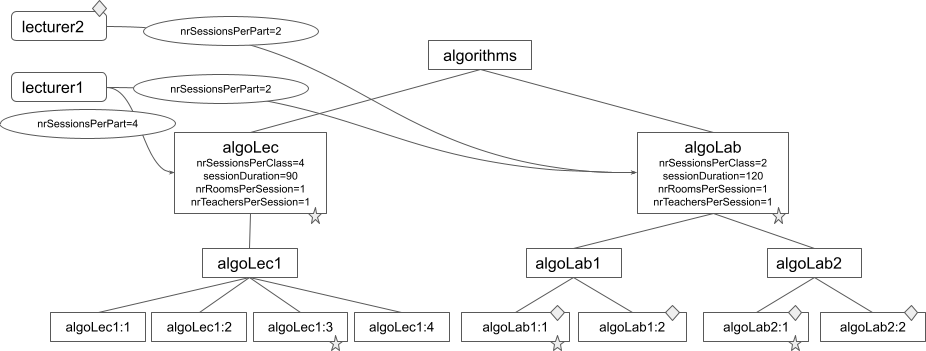
\includegraphics[scale=0.35]{img/utp_rule_1.png}


\newcounter{save_equation}
\setcounter{save_equation}{\value{equation}}
\setcounter{equation}{0}

\renewcommand{\theequation}{R\arabic{equation}}

{\footnotesize{
\begin{flalign}
&\texttt{{\FORBIDDENPERIOD}((<(\TEACHER,{lecturer2},\_)>,9120,9240)}
&\label{rule-example-1}
\\
&\texttt{{\SEQUENCED}(<(\CLASS,\_,\myset{3}),(\PART,{algoLec},\_)>,
<(\CLASS,\_,\myset{1}),(\PART,{algoLab},\_)>)}
&\label{rule-example-2}
\end{flalign}
}}


\setcounter{equation}{0}
\renewcommand{\theequation}{C\arabic{equation}}

%
{
\footnotesize
\begin{flalign}
\nonumber &\texttt{{\FORBIDDENPERIOD}((lecturer2,\{algoLab1:1,algoLab1:2,algoLab2:1,algoLab2:2\}),}\\
 & \texttt{9120,9240)}
&\label{constraint-example-1}
\\
&\texttt{{\SEQUENCED}((algoLec1,\{algoLec1:3\}), (algoLab1,\{algoLab1:1\}))}
&\label{constraint-example-2}
\\
&\texttt{{\SEQUENCED}((algoLec1,\{algoLec1:3\}), (algoLab2,\{algoLab2:1\})}
&\label{constraint-example-3}
\end{flalign}
}
%

\caption{Rules flattening and corresponding constraints on a toy example.}
\label{fig:utp-rule-1}

\setcounter{equation}{\value{save_equation}}
\end{figure}


Figure~\ref{fig:utp-rule-1} illustrates the rules flattening process on a toy example.
Course \texttt{algorithms} is split into a lecture part \texttt{algoLec} and a lab part \texttt{algoLab}.
The lecture part has a single class of 4 sessions taught by \texttt{lecturer1} and the lab part has 2 classes of 2 sessions each taught by \texttt{lecturer1} or \texttt{lecturer2}.
%Figure~\ref{fig:utp-rule-1} illustrates the flattening of the following rules: 
%on a simple model consisting of 2 teachers and & course subdivided into 2 parts, 3 classes and 8 sessions. The first rule forbids a time period for 
Rule~\ref{rule-example-1} %below
requires that \texttt{lecturer2} has no session between slots $9120$ and $9240$, corresponding for instance to 8am and 10am on Tuesday of week 2. % assuming a granularity of 1 minute per time slot. 
%In this rule, $9120$ (resp. $9240$) is the value\footnote{Each possible session schedule is mapped to a single value. All possible values make up the domain of a session.} that corresponds to 8am on Tuesday (resp. 10am on Tuesday) of week 2. 
The selector includes no mask and no filter hence matches with all possible sessions of \texttt{lecturer2} 
as indicated with diamonds on Figure~\ref{fig:utp-rule-1}. 
The resulting domain of e-maps is the singleton $\myset{(lecturer2,\map{\TEACHER}{\SESSION}{lecturer2})}$
and the rule is flattened into a single \texttt{\FORBIDDENPERIOD} constraint (\ref{constraint-example-1}). %$\myset{\map{\TEACHER}{\SESSION}{teacher2}}$.
Rule~\ref{rule-example-2}
%requires that the first practical session in Algorithmic \todo[inline]{Marc : pourquoi algo ?} start after the third lecture.
requires that the first sessions of the labs start after the third lecture.
The two selectors include a filter. The first selector matches with all class sessions of rank 3 in part \texttt{algoLec}, 
and the second matches with all class sessions of rank 1 in part \texttt{algoLab} as indicated with stars on the figure.
The rule is flattened into 2 \texttt{\SEQUENCED} constraints (\ref{constraint-example-2} and \ref{constraint-example-3}) corresponding to the cross product of the e-map domains 
%$\myset{(algoLec1,\map{\RANK}{\SESSION}{3}\cap\map{\PART}{\SESSION}{algoLec})}$
%and $\myset{(algoPra1,\map{\RANK}{\SESSION}{1}\cap\map{\PART}{\SESSION}{algoPra}),(algoPra2,\map{\RANK}{\SESSION}{1}\cap\map{\PART}{\SESSION}{algoPra})}$.
$\myset{(algoLec1,\myset{s\in\SESSION\ |\ \sessionrank{s}=3}\cap\map{\PART}{\SESSION}{algoLec})}$
and $\myset{(algoLab1,\myset{s\in\SESSION\ |\ \sessionrank{s}=1}\cap\map{\PART}{\SESSION}{algoLab}),(algoLab2,\myset{s\in\SESSION\ |\ \sessionrank{s}=1}\cap\map{\PART}{\SESSION}{algoLab})}$.
%------------------------------------------------------------
%------------------------------------------------------------
\subsection{Solution}
\label{sec:solution}
%From introduction
%{\UTP} instances may therefore be used to model subproblems and solution seeds when the whole problem is solved in successive stages (e.g., sequential workflows chaining student sectioning, course scheduling and resource allocation). 
%Since no assumption is made on the computing task, {\UTP} instances may also be used to repair timetables, complete partial timetables or generate full solutions. 

The solution component includes assignment decisions
relating to the choice of slots and resources for sessions,
the placement of students in groups and
the assignment of groups to classes.
The solution hence represented may be partial, even empty,
and does not have to be consistent with the constraints built in the entity model or entailed by the rules.
The support for partial solutions allows to tackle subproblems using separate {\UTP} instances and solution seeds.
For instance, a scheduling instance may be defined on the basis of partial and consistent solutions pre-generated for the student sectioning and resource allocation subproblems.
Likewise, the support for inconsistent solutions is paramount to repair solutions that have become inconsistent due to unforeseen changes.

%As mentioned before, 
Student groups are considered a by-product of student sectioning.
For this reason, groups may only be listed in the solution component, not in the entity model, and defined both by the students they include and the classes they are assigned to. 
This sectioning process is subject to different constraints. 
First, students are partitionned into groups and students are inextricably bound to their group.
Second, a group may only include students with identical course registrations.
Third, group-to-class assignments must comply with any subgroup inclusion constraint stated in the entity model.

%Let ${\SLOT}$ denote the range of slots defining the schedule horizon, $\maptype{\PART}{\SLOT}$ denotes the set of allowed slots defined for each course part in the entity model. 
%$\maptype{\SESSION}{\SLOT}$ shall denote the set of slots assigned to each session in a solution component.
%Let ${\GROUP}$ denote the set of groups defined in a solution, $\maptype{\GROUP}{\STUDENT}$ and $\maptype{\CLASS}{\GROUP}$ shall denote respectively the students making up each group and the groups making up each class.



% %The schema thus allows to cast university timetabling problems either as cumulative or disjunctive scheduling problems that subsume student sectioning or not.


% \paragraph{Paragraph headings} Use paragraph headings as needed.
% \begin{equation}
% a^2+b^2=c^2
% \end{equation}

% For one-column wide figures use
%\begin{figure}
% Use the relevant command to insert your figure file.
% For example, with the graphicx package use
%  \includegraphics{example.eps}
% figure caption is below the figure
%\caption{Please write your figure caption here}
%\label{fig:1}       % Give a unique label
%\end{figure}
%
% For two-column wide figures use
%\begin{figure*}
% Use the relevant command to insert your figure file.
% For example, with the graphicx package use
%  \includegraphics[width=0.75\textwidth]{example.eps}
% figure caption is below the figure
%\caption{Please write your figure caption here}
%\label{fig:2}       % Give a unique label
%\end{figure*}
%
% For tables use
%\begin{table}
% table caption is above the table
%\caption{Please write your table caption here}
%\label{tab:1}       % Give a unique label
% For LaTeX tables use
%\begin{tabular}{lll}
%\hline\noalign{\smallskip}
%first & second & third  \\
%\noalign{\smallskip}\hline\noalign{\smallskip}
%number & number & number \\
%number & number & number \\
%\noalign{\smallskip}\hline
%\end{tabular}
%\end{table}




%------------------------------------------------------------
%------------------------------------------------------------
\subsection{Related work}
\label{sec:related-work}

%Examination timetabling {1999schaerfAIR}: marginal differences with CTP => mandatory attendance for students, different workload constraints for students, can have more than one exam in a room (cumulative room), TAP {2022caselliESWA}: post-allocation of "tutors" to "workshops". BACP {2001castroARXIV,2011chiarandiniJH}: close to maquettage Student sectioning: {2010mullerAOR} => initial vs batch vs online. {2019schindlAOR} CB-CTTP {2010mccollumINFORMS,2012bettinelliAOR,2015bettinelliTOP}: week schedule  with time periods (no session duration), no modeling of student enrolments, hard: same-curriculum/teacher (disjunctive teacher/students), room occupancy, no-overlap(lectures of a course), teacher unavailabilities, soft: room capacity, room stability, ... PE-CTTP {2007lewisITC,2010mccollumINFORMS}: week schedule (45 slots) with time periods (no session duration), student sectioning factored in, each course is a single event (no series of class sessions), students and rooms disjunctive,  New/subsuming models - ITC-2019 {2018mullerPATAT}: - UCTP (survey {2021chenIEEEA}) - {2022zaulirMJFAS,2014aizamNACO} => essentially "new" workload/pattern constraints but probably encodable in ITC. General survey: {2019oudeAOR}:


We highlight here the main differences between the {\UTP} language and the {\ITC} language ({\ITC} for short).

%the two approaches use the same temporal representation but {\ITC} leaves the possibility to configure the granularity of daily slots in each instance (${\DAILYSLOT\in\myset{1\ldots 1440}}$)  while it is set to the minute in {\UTP}. Nevertheless, any granularity may be used in {\UTP} by filtering the series of allowed slots in course parts and by re-scaling session duration and travel time data.
A first difference between the two frameworks lies in the representation of the possible times a class can meet.
In {\UTP}, a class is defined by a single sequence of sessions of equal duration and the problem is to schedule each session.
In {\ITC}, a class is given alternative fixed session schedules ({\texttt{times}} elements in the {\XML} schema) and the problem is to choose one of the schedules for the class.
A schedule is the repetition over a set of weeks of one or more sessions that have the same duration and start on specific days of the week at the same predefined time (daily slot).
The two representations are not reducible to one another.
For instance, alternative schedules using different session durations cannot be modeled in {\UTP}.
Conversely, class schedules where sessions do not necessarily start on the same daily slot cannot be modeled in {\ITC}.
Nevertheless, basic class schedules may be represented in either approach by stating {\ITC} constraints or {\UTP} rules on classes.
For instance, a class meeting every week on the same day and the same daily slot, both being subject to time restrictions, may be modeled using \texttt{\SAMEDAILYSLOT}, \texttt{\WEEKLY} and \texttt{\FORBIDDENPERIOD} constraints.
The implementation of a more comprehensive reduction method %for alternative schedules 
%(based, for instance, on a dedicated {\UTP} predicate) 
will be the subject of future work.

%Another difference lies in the representation of resources and the constraints governing their distribution and allocation.
%On the one hand, 
Second, 
{\ITC} represents alternative course configurations
by introducing an intermediate layer in the course hierarchy 
that sits between courses and parts.
The configurations of a course typically differ in their number of (sub)parts
and are mutually exclusive from a student sectioning standpoint, that is, 
a registered student must be assigned a single configuration and attend all of its parts.
This feature is not currently supported in {\UTP}.
As for resources, {\UTP} explicitly represents lecturers on par with rooms %and allows to specify their workload in each course part %(i.e., the number of sessions to teach)
whereas {\ITC} only models rooms.
{\UTP} also provides the flexibility to allocate different resources within a class 
(and specify lecturer workload in particular) %(i.e., the number of sessions to teach)
whereas the same room must be allocated in {\ITC}.
Additionally, {\UTP} supports multi-resource sessions whereas {\ITC} is restricted to single-room sessions.

Lastly, the two constraint languages present important differences.
While {\ITC} constraint predicates apply to classes,
{\UTP} predicates apply to any set(s) of sessions
and may be used in particular on individual sessions, hence granting finer-grained control.
Besides, {\UTP} rules and the selector language allows to constrain any class of resources or course elements in a concise way.

Lastly, the {\ITC} schema addresses the timetabling problem as a combinatorial optimization problem.
It includes a cost function weighting 4 criteria which respectively penalize the choice of sessions and rooms for the classes, the violations of constraints and the overlapping of sessions per student.
In its current version, the {\UTP} language addresses the problem as a hard constraint satisfaction problem.
The integration of soft constraints and the possibility of aggregating penalties or preferences, either in solution generation or repair contexts, is under investigation.

%Student groups 
% near-identical course structure: no course configuration element
% no time elements in UTP classes. Alternative class times are fixed in ITC
% OK time elements in extension -> unusitable for loosely constrained class programs
% OK impossible to express k weekly slots with different starting slots. In UTP: use sameWeeklySlot with masks.
% OK impossible to enforce different constraints bettwen first period of a course (amorcage) and the rest => ok for us with masks
% KO: times with different #sessions and session length. 
% => solution per session (vs per class) : slot + romms + teachers


%Sectioning:: as itc (parent class)
%Ressources
%- rooms: travel in ITC => using constraint travel in UTP.
%- new: teachers.
%- students: no change.
%- OK groups. Admin and computational needs.
%- Domain constraints
%- by default, all resources are cumultative (explain). Avec contrainte (disjunctive):: no overlap on romms/etc. 
%- allowed slot (applies to all sessions of a part's classes) : ITC via time elements. Adequate for "grid systems". 
%- allowed rooms and allowed teachers (worklaod per part = prescribed number of sessions)
%- single or multi-room/teacher session in UTP.
%- possibly different resources between sessions of a class (unless addiiotnal rules:: sameRoom, sameTeacher, ...)
%Rules language
%- ITC: class-level constraints vs session-level constraints on UTP
%- Labelling: simplifies constraint expression to look up entities
%Solution
%seul ajout: group-to-class and student-to-group
%Résolution: UTP == SAT vs Opt/gestion prefs => pas de priorites, pondérations, etc
%


%------------------------------------------------------------
%------------------------------------------------------------
\section{Modèles \MINIZINC{} et \CHR{}}% des instances \UTP}
\label{sec:model}
\setcounter{equation}{0}
Nous présentons dans cette section deux modèles d'instances {\UTP} développés en \MINIZINC{} et \CHR{}.
Ces modèles mettent en jeu des contraintes relatives
au partitionnement des étudiants en groupes et à l'attribution des groupes aux classes,
à la distribution des ressources sur les séances,
à l'ordonnancement des séances,
et à l'allocation de leurs ressources.
%\davidl{Expliquer transformation du modèle UTP en modèle PPC : "manuel" + built-ins:predicates}
Nous présentons tout d'abord les données d'instance
ainsi que les variables de décision qui sont communes aux deux modèles.
%La table~\ref{table:cp-core-sets} liste les plages d'entiers identifiant les différents ensembles d'objets manipulés.
%(p. ex., ensemble des séancesset of compatible sessions for rooms) and metric properties (e.g., room capacity). 
La table~\ref{table:cp-instance-data} liste les plages d'entiers identifiant les différents ensembles d'objets manipulés et définit les structures utilisées pour représenter les données d'instance.


\begin{table}[!ht]
%\resizebox{\textwidth}{!}{%
\centering
\framebox[\columnwidth][c]{%
\small
\begin{tabularx}{\columnwidth}{>{\hsize=0.01\hsize\linewidth=\hsize}X>{\hsize=1.89\hsize\linewidth=\hsize}X>{\raggedleft\arraybackslash\hsize=.09\hsize\linewidth=\hsize}X}
%\small
%\begin{tabularx}{\columnwidth}{|p{.35\columnwidth}p{.55\columnwidth}|}
%\hline
\SLOT & ensemble des créneaux définissant l'horizon de temps \\
%& (1..(nr\_daily\_slot $\times$ nr\_week\_day $\times$ nr\_week))\\ 
\COURSE & ensemble des cours\\
\PART & ensembles des parties de cours\\
\CLASS & ensembles des classes\\
\SESSION & ensembles des séances\\
\ROOM & ensemble des salles\\
\TEACHER & ensemble des enseignants\\
\GROUP & ensemble des groupes d'étudiants\\
\STUDENT & ensembles des étudiants\\
\hline
%class\_groups               & \\
\multicolumn{2}{p{.9\columnwidth}}{class\_\{sessions,parents\} :} \\
& ensemble des séances (resp. classes parentes) d'une classe \\
%class\_sessions             & \\
%group\_students             & \\
\multicolumn{2}{p{.9\columnwidth}}{part\_\{classes,lecturers, rooms,sessions\} :} \\
 & ensemble des classes (resp. enseignants, salles, séances) d'une partie \\
%part\_lecturers             & \\
%part\_rooms                 & \\
%part\_sessions              & \\
\multicolumn{2}{p{.9\columnwidth}}{room\_sessions :}\\
& ensemble des séances possibles pour une salle\\
\multicolumn{2}{p{.9\columnwidth}}{session\_\{part,class\} : la partie (resp. classe) d'une séance} \\
%session\_class              & \\
\multicolumn{2}{p{.9\columnwidth}}{student\_\{courses,parts\} :}\\
 & les cours (resp. parties) que suit un étudiant \\
%student\_parts              & \\

\multicolumn{2}{p{.9\columnwidth}}{mandatory\_rooms : les salles obligatoires pour une partie} \\
\multicolumn{2}{p{.9\columnwidth}}{single\_room\_sessions : l'ensemble des séances mono-salle} \\
\multicolumn{2}{p{.9\columnwidth}}{capacity : capacité maximum d'une salle ou d'une classe} \\
\multicolumn{2}{p{.9\columnwidth}}{is\_multi\_rooms : indique si une séance est multi-salles} \\
\multicolumn{2}{p{.9\columnwidth}}{length : durée d'une séance} \\
\multicolumn{2}{p{.9\columnwidth}}{part\_room\_use :}\\
 & modalité d'utilisation de salles pour une partie (none, single, multiple) \\
\multicolumn{2}{p{.9\columnwidth}}{rank : rang d'une séance} \\
\multicolumn{2}{p{.9\columnwidth}}{service :} \\
 & nombre de séances à dispenser par enseignant par partie \\
\multicolumn{2}{p{.9\columnwidth}}{teams :} \\
 & nombre d'enseignants requis par séance d'une partie \\
\multicolumn{2}{p{.9\columnwidth}}{virtual : indique si une salle est de capacité illimitée ou non} \\
\multicolumn{2}{p{.9\columnwidth}}{dailyslots : créneaux quotidiens autorisés pour une partie} \\
\multicolumn{2}{p{.9\columnwidth}}{weekdays : journées autorisées pour une partie} \\
\multicolumn{2}{p{.9\columnwidth}}{weeks : semaines autorisées pour une partie} \\
\multicolumn{2}{p{.9\columnwidth}}{nr\_daily\_slots : nombre de créneaux dans une journée} \\
\multicolumn{2}{p{.9\columnwidth}}{nr\_weekly\_slots : nombre de créneaux dans une semaine}\\
%part\_*                     & entité, séance ou valeur associée aux partie de cours\\
%class\_*                    & entité, séance ou valeur associée aux classes\\
%%part\_sessions              & séances d'une partie de cours\\
%%class\_sessions             & séances d'une classe\\
%%part\_ressources            & ressources allouables dans une partie de cours\\
%%part\_daily\_slots          & créneaux quotidiens autorisés pour une partie de cours\\
%%part\_weekdays              & journées hebdomadaires autorisées pour une partie de cours\\
%%part\_weeks                 & semaines autorisées pour une partie de cours\\
%%part\_room\_use             & régime d'utilisation des salles dans une partie de cours\\
%service                     & volume de séances par enseignant et partie de cours\\
%%room\_capacity              & capacité d'accueil d'une salle\\
%%class\_capacity             & effectif maximum d'une classe\\
%*\_capacity                 & seuil de capacité d'une salle ou d'effectif de classe\\
%%room\_max\_use              & \\
%%teacher\_max\_use           & \\
%%group\_max\_use             & \\
%%\end{tabular}
%%}
%%\caption{Données d'instance}
%%\label{table:input-data}
%%\end{table*}
%%
%%\begin{table*}[h]
%%%\resizebox{\textwidth}{!}{%
%%\centering
%%{\footnotesize
%%\begin{tabular}{|rl|}
%%\hline
%session\_*              & entité ou valeur associée à une séance\\
%*\_sessions             & séances associées à une entité\\
%%session\_course         & cours d'une séance\\
%%session\_part           & partie de cours d'une séance\\
%%session\_class          & classe d'une séance\\
%%session\_rank           & rang d'une séance dans sa classe\\
%%session\_length         & durée d'une séance\\
%%team                    & enseignants d'une partie\\
%%room\_sessions          & ensemble des séances possibles pour une salle\\
%%teacher\_sessions       & ensemble des séances possibles pour un enseignant\\
%%group\_sessions         & ensemble des séances possibles pour un groupe\\
%class\_mandatory        & ensemble de salles obligatoires pour une classe\\
%slot\_*                 & conversion d'un créneau vers une durée relative\\
%%slot\_dailyslot         & créneau quotidien caractérisant un créneau\\
%%slot\_weekday           & journée hebdomadaire caractérisant un créneau\\
%%slot\_week              & semaine caractérisant un créneau\\
%\hline
%is\_multi\_rooms        & indique si une séance est multi-salles\\
%has\_mandatory\_rooms   & indique si une séance a des salles obligatoires\\
%nr\_weekly\_slots       & nombre de créneaux dans une semaine\\
%\hline
\end{tabularx}
}
\caption{Données d'instances et fonctions utilitaires}
\label{table:cp-instance-data}
\end{table}

%------------------------------------------------------------
%------------------------------------------------------------

\begin{table*}[!ht]
%\resizebox{\textwidth}{!}{%
\centering
{\small
\begin{tabular}{|lll|}
\hline
array[\STUDENT] of var \GROUP: & $\xstudent$ & groupe attribué à un étudiant\\
array[\CLASS] of var set of \GROUP: & $\xgroup$ & ensemble de groupes alloués à une classe\\
array[\SESSION] of var set of \ROOM: & \xroom & ensemble de salles allouées à une séance\\
array[\SESSION] of var set of \TEACHER: & $\xteacher$ & ensemble d'enseignants alloués à une séance\\
array[\SESSION] of var \SLOT: & $\xslot$ & créneau de départ attribué à une séance\\
\hline
\end{tabular}
}
\caption{Variables de décision (\MINIZINC{})}
\label{table:cp-variables}
\end{table*}



%------------------------------------------------------------
%------------------------------------------------------------
\subsection{Modèle \MINIZINC{}}
\label{sec:model-minizinc}

%------------------------------------------------------------
%------------------------------------------------------------


%\newcolumntype{N}{>{\refstepcounter{rowcntr}\therowcntr}r}
\newcounter{rowcntr}[table]
\renewcommand{\therowcntr}{(\arabic{rowcntr})}
\setcounter{rowcntr}{0}

\begin{table*}[!ht]
\framebox[\textwidth][c]{%
\small
\begin{tabularx}{\textwidth}{>{\hsize=0.01\hsize\linewidth=\hsize}X>{\hsize=1.89\hsize\linewidth=\hsize}X>{\raggedleft\arraybackslash\hsize=.09\hsize\linewidth=\hsize}X}
%\begin{math}\STUDENT = \funcmzn{array\_union}(\xgroup) \end{math} & 
%partition\_set(\xgroup,\begin{math}\STUDENT\end{math}) & \refstepcounter{rowcntr} \therowcntr \label{mzn:grouppartition}\\
%
%
&$\forallmzn(u,v \inmzn \STUDENT \wmzn u\gqmzn v)$ %&\\
%&\hspace*{2,8em}
$(\arraymzn{student\_courses}[u]\neqmzn \arraymzn{student\_courses}[v] \arrowmzn \xstudent[u]\neqmzn \xstudent[v]) $&  \refstepcounter{rowcntr} \therowcntr \label{mzn:studentgrouping}\\
%
%
&$\forallmzn(u \inmzn \STUDENT,p \inmzn \funcmzn{student\_parts}[u])$%&\\
%&\hspace*{2,8em}
$(\existmzn(k \inmzn \arraymzn{part\_classes}[p])(\xstudent[u] \inmzn \xgroup[k]))$& \refstepcounter{rowcntr} \therowcntr \label{mzn:allparts}\\
%forallmzn(u \inmzn \STUDENT, g \inmzn \GROUP)(\xstudent[u] = g \arrowmzn forall(p in \funcmzn{student\_parts}[u])(p = g in  xgroup ))
%
&$\forallmzn(p \inmzn \PART,k1,k2 \inmzn \arraymzn{part\_classes}[p] \wmzn k1\gqmzn k2)$%&\\
%
%\hspace{2cm}all_disjoint
%&\hspace*{2,8em}
$(\xgroup[k1] \intermzn \xgroup[k2]=\{\})$& \refstepcounter{rowcntr} \therowcntr \label{mzn:exclusiveclass}\\
%
%
&$\forallmzn(k1 \inmzn \CLASS, k2 \inmzn \funcmzn{class\_parents}(k1))(\xgroup[k1] \subsetmzn \xgroup[k2])$ &  \refstepcounter{rowcntr} \therowcntr \label{mzn:parent}\\
%
&$\forallmzn(k \inmzn \CLASS)(\arraymzn{maxsize}[k] \geqmzn \summzn(g \inmzn \GROUP)$%&\\
%&\hspace*{2,8em}
$(\funcmzn{bool2int}(g \inmzn \xgroup[k])*\summzn(u \inmzn \STUDENT)(\funcmzn{bool2int}(\xstudent[u]=g)))$ &  \refstepcounter{rowcntr} \therowcntr \label{mzn:classcapacity}\\
% 
%
\hline
%
%
&$\forallmzn(s \inmzn \SESSION)(\xroom[s] \subsetmzn \arraymzn{part\_rooms}[\funcmzn{session\_part}[s]])$& \refstepcounter{rowcntr} \therowcntr \label{mzn:allowedrooms}\\
%
%
&$\forallmzn(s \inmzn \SESSION)(\xteacher[s] \subsetmzn \arraymzn{part\_lecturers}[\funcmzn{session\_part}[s]]) $ &  \refstepcounter{rowcntr} \therowcntr \label{mzn:allowedteachers} \\
%
%
%$\forallmzn(k \inmzn \CLASS)(((\arraymzn{part\_room\_use}[\funcmzn{class\_part}(k)]=\text{none}) \Longleftrightarrow (\xroom[k] = \{\})) $&\\
&$\forallmzn(s \inmzn \SESSION, p \inmzn \PART \wmzn p=\funcmzn{session\_part}[s])($&\\ &\hspace*{2,8em}$(\arraymzn{part\_room\_use}[p]=\text{none} \arrowmzn \xroom[s] = \{\}) \landmzn (\arraymzn{part\_room\_use}[p]=\text{single} \arrowmzn \funcmzn{card}(\xroom[s]) =1)$&\\
&\hspace*{1,4em}$ \landmzn(\arraymzn{part\_room\_use}[p]=\text{multiple} \arrowmzn \funcmzn{card}(\xroom[s]) \leqmzn 1))$
& \refstepcounter{rowcntr} \therowcntr \label{mzn:multiroom}\\
%&$\forallmzn(s \inmzn \SESSION, p \inmzn \PART \wmzn p=\funcmzn{session\_part}[s])($&\\ &\hspace*{2,8em}$(\arraymzn{part\_room\_use}[p]=\text{none} \arrowmzn \xroom[s] = \{\}) $&\\
%&\hspace*{1em}$\landmzn (\arraymzn{part\_room\_use}[p]=\text{single} \arrowmzn \funcmzn{card}(\xroom[s]) = 1)  $&\\
%&\hspace*{1em}$\landmzn(\arraymzn{part\_room\_use}[p]=\text{multiple} \arrowmzn \funcmzn{card}(\xroom[s]) \leqmzn 1))$
%& \refstepcounter{rowcntr} \therowcntr \label{mzn:multiroom}\\
%
%
&$\forallmzn(s \inmzn \SESSION)( \funcmzn{card}(\xteacher[s]) = \funcmzn{team}[\funcmzn{session\_part}[s]])$ & \refstepcounter{rowcntr} \therowcntr 
\label{mzn:multiteacher}\\
%
%
&$\forallmzn(p \inmzn \PART,l \inmzn \arraymzn{part\_lecturers}[p])$%&\\
%&\hspace*{2,8em}
$(\summzn{}(s \inmzn \funcmzn{part\_sessions}[p]))(\funcmzn{bool2int}(l \inmzn \xteacher[s]) = \arraymzn{service}[l,p])) $& \refstepcounter{rowcntr} \therowcntr \label{mzn:partteacherservice}\\
%
%
\hline
%
%
%$\forallmzn(k \inmzn \CLASS)(\xroom[k] \subsetmzn \arraymzn{part\_rooms}[\funcmzn{class\_part}(k))$ & \refstepcounter{rowcntr} \therowcntr  \label{mzn:allowedsrooms}\\
%
%$\forallmzn(s \inmzn \SESSION)(\xteacher[s] \subsetmzn \arraymzn{part\_teachers}[\funcmzn{session\_part}[s]])$  & \refstepcounter{rowcntr} \therowcntr  \label{mzn:allowedsteacher}\\
%
&$\forallmzn(p \inmzn \PART,s \inmzn \funcmzn{part\_sessions}[p])$&\\
&\hspace*{2,8em}$(\funcmzn{week}(\xslot[s]) \inmzn \arraymzn{weeks}[p]\landmzn \funcmzn{weekday}(\xslot[s]) \inmzn \arraymzn{weekdays}[p]\landmzn \funcmzn{dailyslot}(\xslot[s]) \inmzn \arraymzn{dailyslots}[p])$& \refstepcounter{rowcntr} \therowcntr \label{mzn:allowedslots}\\
%&$\forallmzn(p \inmzn \PART,s \inmzn \funcmzn{part\_sessions}(p))$&\\
%&\hspace*{2,8em}$(\funcmzn{week}(\xslot[s]) \inmzn \arraymzn{weeks}[p]$ &\\
%&\hspace*{1em}$\landmzn \funcmzn{weekday}(\xslot[s]) \inmzn \arraymzn{weekdays}[p]$&\\
%&\hspace*{1em}$\landmzn \funcmzn{dailyslot}(\xslot[s]) \inmzn \arraymzn{dailyslots}[p])$& \refstepcounter{rowcntr} \therowcntr \label{mzn:allowedslots}\\
%
%
&$\forallmzn(s \inmzn \SESSION)((\xslot[s] - 1) \divmzn \gconst{nr\_daily\_slots} =(\xslot[s] + \funcmzn{length}[s] - 1) \divmzn \gconst{nr\_daily\_slots})$& \refstepcounter{rowcntr} \therowcntr \label{mzn:nopreemption}\\
%&$\forallmzn(s \inmzn \SESSION)$&\\
%&\hspace*{2,8em}$((\xslot[s] - 1) \divmzn \gconst{nr\_slots\_per\_day} =$&\\
%&\hspace*{2,8em}$(\xslot[s] + \funcmzn{length}[s] - 1) \divmzn \gconst{nr\_slots\_per\_day})$& \refstepcounter{rowcntr} \therowcntr \label{mzn:nopreemption}\\
%
%
&$ \forallmzn(k \inmzn \CLASS, s1,s2 \inmzn \funcmzn{class\_sessions}[k] \wmzn \funcmzn{rank}(s1) \gqmzn \funcmzn{rank}(s2))$ %&\\ 
%&\hspace*{2,8em}
$(\xslot[s1]+\funcmzn{length}[s] \leqmzn \xslot[s2]) $& \refstepcounter{rowcntr} \therowcntr \label{mzn:classsequencing}\\
%
%
%&$\forallmzn(s1 \inmzn \SESSION, r \inmzn \funcmzn{part\_rooms}[\funcmzn{session\_part}[s1]],s2 \inmzn %\funcmzn{room\_sessions}[r] $&\\
%&\hspace*{2,8em}$\wmzn \funcmzn{is\_multi\_rooms}[\funcmzn{session\_part}[s1]]) \landmzn s1 \neqmzn %s2)($&\\
%&\hspace*{3em}$\funcmzn{disjunctive}([\xslot[s1],\xslot[s2]],$&\\
%%
%&\hspace*{3em}$[\funcmzn{bool2int}(r \inmzn \xroom[s1])*\funcmzn{length}[s1],\funcmzn{bool2int}(r %\inmzn \xroom[s2])*\funcmzn{length}[s2]]))$ & \refstepcounter{rowcntr} \therowcntr  %\label{mzn:multiroomscheduling}\\
&$\forallmzn(p \inmzn \PART, s1 \inmzn \funcmzn{part\_sessions}[p], r \inmzn \funcmzn{part\_rooms}[p],s2 \inmzn \funcmzn{room\_sessions}[r] $%&\\
%&\hspace*{2,8em}
$\wmzn \funcmzn{is\_multi\_rooms}[p] \landmzn s1 \neqmzn s2)$&\\
&\hspace*{3em}$(\funcmzn{disjunctive}([\xslot[s1],\xslot[s2]],$&\\
%
&\hspace*{3em}$[\funcmzn{bool2int}(r \inmzn \xroom[s1])*\funcmzn{length}[s1],\funcmzn{bool2int}(r \inmzn \xroom[s2])*\funcmzn{length}[s2]]))$ & \refstepcounter{rowcntr} \therowcntr  \label{mzn:multiroomscheduling}\\
%
%
&$\forallmzn(p \inmzn \PART, s \inmzn \funcmzn{part\_sessions}[p] \wmzn \funcmzn{is\_multi\_rooms}[p])$&\\
&\hspace*{2,8em}$(\summzn(r \inmzn \arraymzn{part\_rooms}[p])(\funcmzn{bool2int}(r \inmzn \xroom[s]) * \arraymzn{capacity}[r])$&\\
&\hspace*{2,8em}$\geqmzn\summzn(g \inmzn \GROUP)(\funcmzn{bool2int}(g \inmzn \xgroup[\funcmzn{session\_class}[s]] )*\funcmzn{card}(\arraymzn{group\_students}[g])))$& \refstepcounter{rowcntr} \therowcntr \label{mzn:multiroomcapacity}\\
%
%
%$\forallmzn(s \inmzn \SESSION, r \inmzn \funcmzn{session\_rooms}[s])($&\\
%\multicolumn{1}{|c}{$\arraymzn{room\_capacity}[r] \geq sum(g \inmzn %\funcmzn{session\_group}[s])(\funcmzn{card}(\arraymzn{group\_students}[g]))))$} & \refstepcounter{rowcntr} \therowcntr  
%\label{mzn:cumulativeroomcapacity}\\
%
%
&$\forallmzn(p \inmzn \PART, s \inmzn \funcmzn{part\_sessions}[p])(\funcmzn{mandatory\_rooms}[p] \subsetmzn \xroom[s])$& \refstepcounter{rowcntr} \therowcntr \label{mzn:mandatoryrooms}\\
%
%
%&$\forallmzn(r \inmzn \ROOM  \wmzn \notmzn(\funcmzn{virtual}[r]))$&\\
%&\hspace*{2,8em}$(\funcmzn{cumulative}([\xslot[s] | s \inmzn \funcmzn{room\_sessions}[r]],$&\\
%&\hspace*{2,8em}$[\funcmzn{bool2int}(r \inmzn \xroom[s])* \funcmzn{length}[s] | s \inmzn \funcmzn{room\_sessions}[r]  ],$&\\
%&\hspace*{3em}$[\summzn(g \inmzn \GROUP)(\funcmzn{bool2int}(g \inmzn \xgroup[\funcmzn{session\_class}[s]])) * \summzn(u \inmzn \STUDENT)($&\\
%&$\funcmzn{bool2int}(g = \xstudent[u]))| s \inmzn \funcmzn{room\_sessions}[r]],\arraymzn{capacity}[r]))$& \refstepcounter{rowcntr} \therowcntr  
%\label{mzn:roomuse}\\
&$\forallmzn(r \inmzn \ROOM  \wmzn \notmzn(\funcmzn{virtual}[r]))(\funcmzn{let \{}\funcmzn{set of \SESSION: RS= room\_sessions}[r]\intermzn\funcmzn{single\_room\_sessions;}\}\inmzn$&\\
&\hspace*{2,8em}$(\funcmzn{cumulative}([\xslot[s] | s \inmzn RS],[\funcmzn{bool2int}(r \inmzn \xroom[s])* \funcmzn{length}[s] | s \inmzn RS],$&\\
%&$\forallmzn(r \inmzn \ROOM  \wmzn \notmzn(\funcmzn{virtual}[r]))($&\\
%&\hspace*{2,8em}$\funcmzn{let \{}\funcmzn{set of \SESSION: RS= room\_sessions}[r]\intermzn\funcmzn{single\_room\_sessions;}\}\inmzn$&\\
%&\hspace*{2,8em}$(\funcmzn{cumulative}([\xslot[s] | s \inmzn RS],[\funcmzn{bool2int}(r \inmzn \xroom[s])* \funcmzn{length}[s] | s \inmzn RS],$&\\
%&\hspace*{2,8em}$(\funcmzn{cumulative}([\xslot[s] | s \inmzn RS],$&\\
%&\hspace*{2,8em}$[\funcmzn{bool2int}(r \inmzn \xroom[s])* \funcmzn{length}[s] | s \inmzn RS],$&\\
&\hspace*{2,8em}$[\summzn(g \inmzn \GROUP)(\funcmzn{bool2int}(g \inmzn \xgroup[\funcmzn{session\_class}[s]])) * \summzn(u \inmzn \STUDENT)($&\\
&$\funcmzn{bool2int}(g = \xstudent[u]))| s \inmzn RS],\arraymzn{capacity}[r]))$& \refstepcounter{rowcntr} \therowcntr \label{mzn:roomuse}\\
%&\hspace*{2em}$[\summzn(g \inmzn \GROUP)(\funcmzn{bool2int}(g \inmzn \xgroup[\funcmzn{session\_class}[s]])) * \summzn(u \inmzn \STUDENT)($&\\
%&$\funcmzn{bool2int}(g = \xstudent[u]))| s \inmzn RS],\arraymzn{capacity}[r]))$& \refstepcounter{rowcntr} \therowcntr \label{mzn:roomuse}\\
%
%
%\forallmzn(t \inmzn \TEACHER)(\funcmzn{cumulative}( & \\
%\multicolumn{1}{|c}{$[\xslot[s] | s \inmzn \funcmzn{teacher\_sessions}(t)],[\funcmzn{bool2int}(t \subsetmzn \xteacher[s])* \funcmzn{session\_length}[s] | s \inmzn \funcmzn{teacher\_sessions}(t)],$}&\\
%\multicolumn{1}{|c}{$[1| s \inmzn \funcmzn{teacher\_sessions}(t)],teacher\_max\_use[t])))$}& \refstepcounter{rowcntr} \therowcntr  
%\label{mzn:teacheruse}\\
%
%
%$\forallmzn(g \inmzn \GROUP)(\funcmzn{cumulative}($&\\
%\multicolumn{1}{|c}{$[\xslot[s] | s \inmzn \funcmzn{group\_sessions}(g)],[\funcmzn{session\_length}[s] | s \inmzn \funcmzn{group\_sessions}(g)],$}&\\
%\multicolumn{1}{|c}{$[1| s \inmzn \funcmzn{group\_sessions}(g)],group\_max\_use[g])))$}& \refstepcounter{rowcntr} \therowcntr  
%\label{mzn:groupuse}\\
%
%
\hline
%
%
&$\FORBIDDENPERIOD((r,S'),h1,h2) = \forallmzn(i \inmzn S')( r \inmzn \xroom[i] \arrowmzn (\xslot[i]+\funcmzn{length}[i] \geqmzn h_1 \lormzn  \xslot[i]\lqmzn h_2)) $& \refstepcounter{rowcntr} \therowcntr \label{mzn:forbiddenperiod}\\
%&$\FORBIDDENPERIOD((r,S'),h1,h2) = \forallmzn(i \inmzn S')($&\\
%&\hspace*{2,8em}$ r \inmzn \xroom[i] \arrowmzn (\xslot[i]+\funcmzn{length}[i] \geqmzn h_1 \lormzn  \xslot[i]\lqmzn h_2)) $& \refstepcounter{rowcntr} \therowcntr \label{mzn:forbiddenperiod}\\
%
%
&$\SAMEWEEKDAY((r,S')) = \forallmzn(i,j \inmzn S' \wmzn i\gqmzn j)($&\\
&\hspace*{2,8em}$ (r\inmzn \xroom[i] \intermzn \xroom[j]) \arrowmzn(\xslot[i] \divmzn \gconst{nr\_weekly\_slots}=\xslot[j] \divmzn  \gconst{nr\_weekly\_slots}))$ & \refstepcounter{rowcntr} \therowcntr 
\label{mzn:sameweekday}\\
%&$\SAMEWEEKDAY((r,S')) = \forallmzn(i,j \inmzn S' \wmzn i\gqmzn j)($&\\
%&\hspace*{2,8em}$ (r\inmzn \xroom[i] \intermzn \xroom[j]) \arrowmzn $&\\
%&\hspace*{2,8em}$(\xslot[i] \divmzn \gconst{nr\_weekly\_slots}=\xslot[j] \divmzn  \gconst{nr\_weekly\_slots}))$ & \refstepcounter{rowcntr} \therowcntr \label{mzn:sameweekday}\\
%
%
&$\SAMEROOMS((r,S')) = \forallmzn(i,j \inmzn S' \wmzn i\gqmzn j)(($&\\
&\hspace*{2,8em}$r\inmzn \xroom[i] \intermzn \xroom[j]) \arrowmzn \xroom[i] = \xroom[j])$ & \refstepcounter{rowcntr} \therowcntr  \label{mzn:samerooms}\\
%
%
&$\SEQUENCED((r1,S1),(r2,S2)) = \forallmzn(i \inmzn S1,j \inmzn S2)($&\\
&\hspace*{3em}$(r1\inmzn \xroom[i] \landmzn r2\inmzn \xroom[j]) \arrowmzn\xslot[i]\texttt{+}\funcmzn{length}[i] \geqmzn \xslot[j])$ & \refstepcounter{rowcntr} \therowcntr \label{mzn:sequenced}\\
%
%
&$\NOOVERLAP((r,S'))=\funcmzn{disjunctive}([\xslot[i]|i \inmzn S'],[\funcmzn{length}[i]*\funcmzn{bool2int}(r \inmzn \xroom[i])|i \inmzn S'])$ & \refstepcounter{rowcntr} \therowcntr \label{mzn:nooverlap}\\
%
%&$\NOOVERLAP((r,S'))=$&\\
%&\hspace*{2,8em}$\funcmzn{disjunctive}([\xslot[i]|i \inmzn S'],[\funcmzn{length}[i]*\funcmzn{bool2int}(r \inmzn \xroom[i])|i \inmzn S'])$ & \refstepcounter{rowcntr} \therowcntr \label{mzn:nooverlap}\\
%
\end{tabularx}%
}%
\caption{Contraintes et prédicats du modèle }
\label{table:mzn-contraintes}
\end{table*}

%\corentin{}


% \begin{table*}[!ht]
% %\resizebox{\textwidth}{!}{%
% \small
% \centering
% \begin{tabular}{|lr|}
% \hline
% %\begin{math}\STUDENT = \funcmzn{array\_union}(\xgroup) \end{math} & 
% %partition\_set(\xgroup,\begin{math}\STUDENT\end{math}) & \refstepcounter{rowcntr} \therowcntr \label{ctr:grouppartition}\\
% %
% %
% $\forallmzn(u,v \inmzn \STUDENT \wmzn u<v)(%$&\\
% ( \arraymzn{student\_courses}[u]!=\arraymzn{student\_courses}[v] ) \arrowmzn ( \xstudent[u]!=\xstudent[v] )) $&  \refstepcounter{rowcntr} \therowcntr \label{ctr:studentgrouping}\\
% %
% %
% $\forallmzn(u \inmzn \STUDENT,p \inmzn \funcmzn{student\_parts}(u))(\existmzn(k \inmzn \arraymzn{part\_classes}[p])(\xstudent[u] \inmzn \xgroup[k])))$& \refstepcounter{rowcntr} \therowcntr \label{ctr:allparts}\\
% %forallmzn(u \inmzn \STUDENT, g \inmzn \GROUP)(\xstudent[u] = g \arrowmzn forall(p in \funcmzn{student\_parts}(u))(p = g in  xgroup ))
% %
% $\forallmzn(p \inmzn \PART,k_1,k_2 \inmzn \arraymzn{part\_classes}[p] \wmzn k_1<k_2)($%&\\
% %
% %\hspace{2cm}all_disjoint
% $ \xgroup[k_1] \intermzn \xgroup[k_2] = \{\})$& \refstepcounter{rowcntr} \therowcntr \label{ctr:exclusiveclass}\\
% %
% %
% $\forallmzn(k_1 \inmzn \CLASS, k_2 \inmzn \funcmzn{class\_parent}(k_1))(\xgroup[k_1] \subsetmzn \xgroup[k_2])$ &  \refstepcounter{rowcntr} \therowcntr \label{ctr:parent}\\
% %
% $\forallmzn(k \inmzn \CLASS)(\arraymzn{  class\_capacity}[k] \geqmzn \summzn(g \inmzn \GROUP)( \funcmzn{ bool2int}(g \inmzn \xgroup[k]) * \summzn(u \inmzn \STUDENT)(\funcmzn{bool2int}(\xstudent[u] == g))))$ &  \refstepcounter{rowcntr} \therowcntr \label{ctr:classcapacity}\\
% % 
% %
% \hline
% %
% %
% $\forallmzn(s \inmzn \SESSION)(\xroom[s] \subsetmzn \arraymzn{part\_rooms}[\funcmzn{session\_part}(s)])$& \refstepcounter{rowcntr} \therowcntr \label{ctr:allowedrooms}\\
% %
% %
% $\forallmzn(s \inmzn \SESSION)(\xteacher[s] \subsetmzn \arraymzn{part\_teachers}[\funcmzn{session\_part}(s)]) $ &  \refstepcounter{rowcntr} \therowcntr \label{ctr:allowedteachers} \\
% %
% %
% %$\forallmzn(k \inmzn \CLASS)(((\arraymzn{part\_room\_use}[\funcmzn{class\_part}(k)]=\text{none}) \Longleftrightarrow (\xroom[k] = \{\})) $&\\
% $\forallmzn(s \inmzn \SESSION)((( $\hspace{1,3cm}$\arraymzn{part\_room\_use}[\funcmzn{session\_part}(s)]=\text{none}) \equimzn (\xroom[s] = \{\})) $&\\
% \multicolumn{1}{|c}{$\landmzn ((\arraymzn{part\_room\_use}[\funcmzn{session\_part}(s)]=\text{single}) \arrowmzn (\funcmzn{card}(\xroom[s]) = 1))  $}&\\
% \multicolumn{1}{|c}{$\landmzn((\arraymzn{part\_room\_use}[\funcmzn{session\_part}(s)]=\text{multiple}) \arrowmzn (\funcmzn{card}(\xroom[s])>=1)))$}
% & \refstepcounter{rowcntr} \therowcntr 
% \label{ctr:multiroom}\\
% %
% %
% $\forallmzn(s \inmzn \SESSION)( \funcmzn{card}(\xteacher[s]) = \funcmzn{teacher\_per\_session}[s])$ & \refstepcounter{rowcntr} \therowcntr 
% \label{ctr:multiteacher}\\
% %
% %
% \davidl{use GCC for (10)}
% $\forallmzn(p \inmzn \PART,t \inmzn \arraymzn{part\_teachers}[p])(\summzn{}(s \inmzn \funcmzn{part\_sessions}(p))(\funcmzn{bool2int}(t \inmzn \xteacher[s])) = \arraymzn{part\_teacher\_service}[p,t]) $& \refstepcounter{rowcntr} \therowcntr 
% \label{ctr:partteacherservice}\\
% %
% %
% \hline
% %
% %
% %$\forallmzn(k \inmzn \CLASS)(\xroom[k] \subsetmzn \arraymzn{part\_rooms}[\funcmzn{class\_part}(k))$ & \refstepcounter{rowcntr} \therowcntr  \label{ctr:allowedsrooms}\\
% %
% %$\forallmzn(s \inmzn \SESSION)(\xteacher[s] \subsetmzn \arraymzn{part\_teachers}[\funcmzn{session\_part}(s)])$  & \refstepcounter{rowcntr} \therowcntr  \label{ctr:allowedsteacher}\\
% %
% $\forallmzn(p \inmzn \PART,s \inmzn \funcmzn{part\_sessions}(p))(($\hspace{0.5cm}$\funcmzn{slot\_week}(\xslot[s]) \inmzn \arraymzn{part\_weeks}[p])$ &\\
%   \multicolumn{1}{|c}{$\landmzn (\funcmzn{slot\_weekday}(\xslot[s]) \inmzn \arraymzn{part\_days}[p])$} &\\
%   \multicolumn{1}{|c}{$\landmzn (\funcmzn{slot\_dailyslot}(\xslot[s]) \inmzn \arraymzn{part\_dailyslots}[p]))$}& \refstepcounter{rowcntr} \therowcntr 
% \label{ctr:allowedslots}\\
% %
% %
% $\forallmzn(s \inmzn \SESSION)((\xslot[s] - 1) \divmzn \gconst{nr\_slots\_per\_day} = (\xslot[s] + \funcmzn{session\_length}(s) - 1) \divmzn \gconst{nr\_slots\_per\_day})$& \refstepcounter{rowcntr} \therowcntr 
% \label{ctr:nopreemption}\\
% %
% %
% $ \forallmzn(k \inmzn \CLASS, s_1,s_2 \inmzn \funcmzn{class\_sessions}[k] \wmzn \funcmzn{session\_rank}(s_1)<\funcmzn{session\_rank}(s_2) )$ &\\
% \multicolumn{1}{|c}{$(\xslot[s_1]+\funcmzn{session\_length}(s) \leqmzn \xslot[s_2])) $}& \refstepcounter{rowcntr} \therowcntr 
% \label{ctr:classsequencing}\\
% %
% %
% $\forallmzn( s \inmzn \SESSION, r \inmzn \funcmzn{class\_rooms}(\funcmzn{session\_class}(s)),s_p \inmzn \funcmzn{room\_sessions}(r)] \wmzn \funcmzn{is\_multi\_rooms}(s)) \landmzn s != s_p)($&\\
% \multicolumn{1}{|c}{$\funcmzn{disjunctive}([\xslot[s],\xslot[s_p] ],$}&\\
% %
% \multicolumn{1}{|c}{$[\funcmzn{bool2int}(r \inmzn \xroom[s])* \funcmzn{session\_length}(s),\funcmzn{bool2int}(r \inmzn \xroom[s_p])* \funcmzn{session\_length}(s_p)])))$} & \refstepcounter{rowcntr} \therowcntr  \label{ctr:multiroomscheduling}\\
% %
% %
% $\forallmzn(s \inmzn \SESSION \wmzn \funcmzn{is\_multi\_rooms}(s))( \summzn(r \inmzn \arraymzn{session\_rooms}[s])($&\\
% $\funcmzn{bool2int}(r \inmzn \xroom[s]) * \arraymzn{room\_capacity}[r]) \geqmzn \summzn(g \inmzn \arraymzn{class\_group}[\funcmzn{session\_class}(s)])(\funcmzn{card}(\arraymzn{group\_students}[g]))$& \refstepcounter{rowcntr} \therowcntr  
% \label{ctr:multiroomcapacity}\\
% %
% %
% %$\forallmzn(s \inmzn \SESSION, r \inmzn \funcmzn{session\_rooms}(s))($&\\
% %\multicolumn{1}{|c}{$\arraymzn{room\_capacity}[r] \geq sum(g \inmzn %\funcmzn{session\_group}(s))(\funcmzn{card}(\arraymzn{group\_students}[g]))))$} & \refstepcounter{rowcntr} \therowcntr  
% %\label{ctr:cumulativeroomcapacity}\\
% %
% %
% $\forallmzn(s \inmzn \SESSION \wmzn \funcmzn{has\_mandatory\_room}(s))(\xroom[s] \intermzn \funcmzn{session\_mandatory}[s] != \{\})$& \refstepcounter{rowcntr} \therowcntr 
% \label{ctr:mandatoryrooms}\\
% %
% %
% $\forallmzn(r \inmzn \ROOM)($&\\
% \multicolumn{1}{|c}{$\funcmzn{cumulative}([\xslot[s] | s \inmzn \funcmzn{room\_sessions}(r)],[\funcmzn{bool2int}(r \inmzn \xroom[s])* \funcmzn{session\_length}(s) | s \inmzn \funcmzn{room\_sessions}(r)  ],$}&\\
% \multicolumn{1}{|c}{$[\summzn(g \inmzn \GROUP)(\funcmzn{bool2int}(g \inmzn \xgroup[\funcmzn{session\_class}(s)]) * \summzn(u \inmzn \STUDENT)(\funcmzn{bool2int}(g = \xstudent[u]))| s \inmzn \funcmzn{room\_session}(r)],$}&\\
% $\arraymzn{room\_capacity}(r))))$& \refstepcounter{rowcntr} \therowcntr  
% \label{ctr:roomuse}\\
% %
% %
% %\forallmzn(t \inmzn \TEACHER)(\funcmzn{cumulative}( & \\
% %\multicolumn{1}{|c}{$[\xslot[s] | s \inmzn \funcmzn{teacher\_sessions}(t)],[\funcmzn{bool2int}(t \subsetmzn \xteacher[s])* \funcmzn{session\_length}(s) | s \inmzn \funcmzn{teacher\_sessions}(t)],$}&\\
% %\multicolumn{1}{|c}{$[1| s \inmzn \funcmzn{teacher\_sessions}(t)],teacher\_max\_use[t])))$}& \refstepcounter{rowcntr} \therowcntr  
% %\label{ctr:teacheruse}\\
% %
% %
% %$\forallmzn(g \inmzn \GROUP)(\funcmzn{cumulative}($&\\
% %\multicolumn{1}{|c}{$[\xslot[s] | s \inmzn \funcmzn{group\_sessions}(g)],[\funcmzn{session\_length}(s) | s \inmzn \funcmzn{group\_sessions}(g)],$}&\\
% %\multicolumn{1}{|c}{$[1| s \inmzn \funcmzn{group\_sessions}(g)],group\_max\_use[g])))$}& \refstepcounter{rowcntr} \therowcntr  
% %\label{ctr:groupuse}\\
% %
% %
% \hline
% %
% %
% $\FORBIDDENPERIOD((e,S_p),h_1,h_2) = \forallmzn(i \inmzn S_p )( e \inmzn \xroom[i] \arrowmzn (\xslot[i] < h_1) \landmzn  (\xslot[i]>h_2)) $& \refstepcounter{rowcntr} \therowcntr 
% \label{ctr:forbiddenperiod}\\
% %
% %
% $\SAMEWEEKDAY((e,S_p)) = \forallmzn(i,j \inmzn S_p \wmzn i<j)($&\\
% \multicolumn{1}{|c}{$ (e\inmzn \xroom[i] \landmzn e\inmzn \xroom[j]) \arrowmzn (\xslot[i] \divmzn nr\_weekly\_slots) = (\xslot[j] \divmzn nr\_weekly\_slots))$} & \refstepcounter{rowcntr} \therowcntr 
% \label{ctr:sameweekday}\\
% %
% %
% $\SAMEROOMS((e,S_p)) = \forallmzn(s_1,s_2 \inmzn S_p \wmzn s_1<s_2 )(($&\\
% %
% \multicolumn{1}{|c}{$e\inmzn \xroom[s_1] \landmzn e\inmzn \xroom[s_2]) \arrowmzn \xroom[s_1] = \xroom[s_2])$} & \refstepcounter{rowcntr} \therowcntr 
% \label{ctr:samerooms}\\
% %
% %
% $\SEQUENCED((e_1,S_1),(e_2,S_2)) = \forallmzn(i \inmzn S_1,j \inmzn S_2)($&\\
% \multicolumn{1}{|c}{$(e_1\inmzn \xroom[i] \landmzn e_2\inmzn \xroom[j]) \arrowmzn \xslot[i]+\funcmzn{session\_length}(i) \leqmzn \xslot[j])$} & \refstepcounter{rowcntr} \therowcntr 
% \label{ctr:sequenced}\\
% %
% %
% $\NOOVERLAP((e_1,S_1))= \funcmzn{disjunctive}([\xslot[s]|s \inmzn S_1 ],[\funcmzn{session\_length}(s)*\funcmzn{bool2int}(e_1 \inmzn \xroom[s])|s \inmzn S_1])$ & \refstepcounter{rowcntr} \therowcntr 
% \label{ctr:nooverlap}\\
% \hline
% \end{tabular}
% %}
% \caption{Contraintes et prédicats du modèle \MINIZINC{}}
% \label{table:mzn-contraintes}
% \end{table*}

%------------------------------------------------------------
%------------------------------------------------------------
%\subsection{Student Sectioning}
%\label{sec:model-sectioning}

{\MINIZINC} est un langage de modélisation haut-niveau de problèmes d'optimisation sous contraintes \cite{MZN,MINIZINC}. 
Les modèles {\MINIZINC} sont traduits dans le langage cible {\FLATZINC} \cite{FLATZINC} qui permet d'interfacer différents types de solveurs dont les solveurs de programmation par contraintes sur domaines finis tels  {\GECODE} \cite{GECODE}.
{\MINIZINC} intègre de nombreuses contraintes globales et le modèle {\UTP} présenté en Table~\ref{table:mzn-contraintes} et utilisant les variables de décision présentée en Table~\ref{table:cp-variables} s'appuie sur quelques contraintes dédiées aux problèmes d'ordonnancement.

%\davidl{Expliquer fichier DZN + fichier MZN avec implémentation prédicats UTP}
Les contraintes de sectionnement répartissent
les étudiants dans les groupes et assigne chacun de ces groupes à différentes classes 
conformément aux règles de sectionnement et aux seuils d'effectifs.
%La contrainte~\ref{mzn:grouppartition} partitionne les étudiants en groupes.
La contrainte \ref{mzn:studentgrouping} n'autorise le regroupement
d'étudiants que s'ils sont inscrits aux mêmes cours.
\ref{mzn:allparts} impose que tout étudiant, assimilé à son groupe, assiste à toute partie de cours dans lequel il est inscrit.
\ref{mzn:exclusiveclass} assure que les classes d'une partie de cours n'ont aucun groupe en commun.
\ref{mzn:parent} implémente la relation de parenté entre classes.
Enfin, \ref{mzn:classcapacity} vérifie que l'effectif cumulé des groupes attribués à une classe ne dépasse pas le seuil autorisé. 
%A noter que cette contrainte utilise des variables auxiliaires pseudo-booléennes.

%------------------------------------------------------------
%------------------------------------------------------------
%\subsubsection{Resource Distribution}
%\label{sec:model-distribution}

La distribution des ressources s'appuie sur des contraintes de domaine, de cardinalité et de sommes.
Les contraintes~\ref{mzn:allowedrooms} et \ref{mzn:allowedteachers} définissent les salles et enseignants allouables à chaque séance.
\ref{mzn:multiroom} contraint le nombre de salles allouées à une séance selon que sa partie de cours est sans salles, mono-salle, ou multi-salles.
\ref{mzn:multiteacher} attribue le nombre attendu d'enseignants à chaque séance
et \ref{mzn:partteacherservice} vérifie que chaque enseignant dispense le volume de séances requis par partie de cours où il est pré-positionné.

%------------------------------------------------------------
%------------------------------------------------------------
%\subsubsection{Session Scheduling and Resource Allocation}
%\label{sec:model-scheduling}

La programmation des séances et l'allocation des ressources met en jeu des contraintes de positionnement, de séquencement, de non-chevauchement et de capacité. 
%Constraint~\ref{mzn:allowedslots} defines the allowed slots per session
%and 
La contrainte~\ref{mzn:allowedslots} définit les créneaux autorisés pour chaque séance.
\ref{mzn:nopreemption} interdit qu'une séance soit à cheval sur 2 journées. 
\ref{mzn:classsequencing} séquence les séances d'une classe selon leur rangs.
Les contraintes \ref{mzn:multiroomscheduling} et \ref{mzn:multiroomcapacity} modélisent les séances multi-salles et l'accès exclusif à leurs ressources.
\ref{mzn:multiroomscheduling} impose qu'une ressource allouée à une séance multi-salles soit disjonctive le temps de son utilisation.
\ref{mzn:multiroomcapacity} assure que le nombre d'étudiants attendus n'excède pas la capacité cumulée des salles allouées.
À noter que cette contrainte est purement quantitative et autorise toute répartition d'étudiants dans les salles indépendamment de la structure de groupes.
\ref{mzn:mandatoryrooms} modélise les salles à allouer obligatoirement à toute séance d'une partie de cours.
\ref{mzn:roomuse} modélise la contrainte de capacité cumulative qui s'applique par défaut à toute salle allouée hors séances multi-salles.
%\ref{mzn:groupuse}

%------------------------------------------------------------
%------------------------------------------------------------

%\subsubsection{{\UTP} Predicates}
%\label{sec:model-predicates}

%%%%{\ADJACENTROOMS}
%%%%{\ATMOSTDAILY}
%%%%{\ATMOSTWEEKLY}
%%%%{\TRAVEL}
%{\FORBIDDENPERIOD}
%{\NOOVERLAP}
%%%%{\SAMEDAILYSLOT}
%%%%{\SAMEDAY}
%{\SAMEROOMS}
%%%%{\SAMESLOT}
%%%%{\SAMESTUDENTS}
%%%%{\SAMETEACHERS}
%{\SAMEWEEKDAY}
%%%%{\SAMEWEEKLYSLOT}
%%%%{\SAMEWEEK}
%{\SEQUENCED}
%%%%{\TEACHERDISTRIBUTION}
%%%%{\WEEKLY}

%Due to lack of space, we just present a few {\UTP} constraint predicates, namely,
La table~\ref{table:mzn-contraintes} présente les variantes de quelques prédicats \UTP{} dans le cas où les entités ciblées sont des salles.
%, respectivement,
%\texttt{\FORBIDDENPERIOD} (\ref{mzn:forbiddenperiod}),
%\texttt{\SAMEWEEKDAY} (\ref{mzn:sameweekday}), 
%\texttt{\SAMEROOMS} (\ref{mzn:samerooms}),
%\texttt{\NOOVERLAP} (\ref{mzn:nooverlap}) 
%et \texttt{\SEQUENCED} (~\ref{mzn:sequenced}).
%Note that \texttt{\FORBIDDENPERIOD} accepts start and end point parameters.
\ref{mzn:forbiddenperiod} implémente le prédicat \texttt{\FORBIDDENPERIOD} qui prend en paramètres les 2 créneaux modélisant la période interdite. 
\ref{mzn:sameweekday}, \ref{mzn:samerooms} et \ref{mzn:sequenced} modélisent de manière directe les prédicats \texttt{\SAMEWEEKDAY}, \texttt{\SAMEROOMS} et \texttt{\SEQUENCED}.
\ref{mzn:nooverlap} implémente le prédicat \texttt{\NOOVERLAP} en s'appuyant sur la contrainte globale \texttt{disjunctive}. %de \MINIZINC{}.


% Note that entailed constraints may be enforced. 
% For instance, a room $r$ is necessarily disjunctive if a non-overlapping constraint is enforced on its set of compatible sessions, %\footnote{
%Il faut noter que des contraintes peuvent être renforcés. 
%Par exemple, une salle $r$ est nécessairement disjonctive si une contrainte de non-chevauchement est appliquée à son ensemble de sessions possibles, c'est-à-dire si l'instance inclut la contrainte ${no\_overlap}$.
% i.e., if the instance includes constraint ${no\_overlap}((r,\map{\ROOM}{\SESSION}{r}))$.
% If so, the default cumulative capacity constraint may be safely replaced with  Constraint~\ref{mzn:disjunctiveroomcapacity} for such resources where
% $\disjunctiverooms\subseteq{\ROOM}$         denotes the set of disjunctive rooms.
%Dans ce cas, la contrainte cumulative par défaut peut être remplacée en toute sécurité par la contrainte~\ref{mzn:disjunctiveroomcapacity} pour les ressources concernés.

\subsection{Modèle \CHR{}}

{\it Constraint Handling Rules} ({\CHR}) \cite{Fruhwirth_JLP_98,Fruhwirth_CHR_09} est un langage à base de règles d’inférence à chaînage avant qui remplacent les contraintes du problème
par d’autres plus simples jusqu’à la résolution complète.
\CHR\ est un langage spécialisé permettant de définir des contraintes déclaratives au sens de la programmation logique par contraintes \cite{VanHentenryck_ker_91,Jaffar_Malher_JLP_94}.
\CHR\ est une extension de langage qui permet d'introduire des contraintes définies par l'utilisateur, c'est-à-dire des prédicats du premier ordre, dans un langage hôte donné tel que {\PROLOG}, {\LISP}, {\JAVA}, ou {\C}/{\CPP}.
Il a ensuite été étendu à {\CHR}\ensuremath{^{\vee}} \cite{Abdennadher_Schutz_FQAS_98} qui introduit le \emph{don't know} \cite{Betz_Fruhwirth_TCL_13}.
Ce non-déterminisme est offert gratuitement lorsque le langage hôte est {\PROLOG} et il permet de spécifier facilement des problèmes de la classe de complexité {\NP}. Pour modéliser et résoudre les instances {\UTP} avec le langage {\CHR}, nous utilisons le solveur {\CHRPP}~\cite{barichard_stephan_2019} (pour Constraint Handling Rules in {\CPP}), qui est une intégration efficace de {\CHR} dans le langage de programmation \texttt{C++}.\\

%\marc{paragraphe parsing}
Le modèle \CHR{} est instancié à la lecture de l'instance au format \JSON{}.
Le modèle d'entité est d'abord défini, puis les contraintes issues des règles sont déclarées et enfin les domaines des variables sont mis à jour si une partie solution est fourniée, avant de lancer la résolution de l'instance.
%
Le modèle complet pour \CHRPP\ est trop long pour être détaillé ici\footnote{Le lecteur intéressé peut télécharger les sources du modèle~\cite{uspSite}}. Nous donnons dans le tableau~\ref{table:contrainte-tab-chr} la liste des contraintes prises en compte par le solveur. Les variables de décisions devant être instanciées sont données au tableau~\ref{table:chr-variables}. Elles sont en grande partie similaires à celles du modèle \MINIZINC, seules les variables de fin de séances sont ajoutées.\\

\begin{table*}[!ht]
\framebox[\linewidth][c]{%
\small
\begin{tabular}{ll}
array[\SESSION] of var set of \ROOM: $\xroom$ & ensemble de salles allouées à une séance\\
array[\SESSION] of var set of \TEACHER: $\xteacher$ & ensemble d'enseignants alloués à une séance\\
array[\SESSION] of int \SLOT: $\xslotstart$ & créneau de départ attribué à une séance\\
array[\SESSION] of int \SLOT: $\xslotend$ & créneau de fin attribué à une séance\\
\end{tabular}%
}
\caption{Variables de décision (\CHR)}
\label{table:chr-variables}
\end{table*}

\newcounter{rowcntrchr}[table]
\setcounter{rowcntrchr}{0}
\renewcommand{\therowcntrchr}{(\arabic{rowcntrchr})}

\begin{table*}[!ht]
\framebox[\textwidth][c]{%
\small
\begin{tabularx}{\textwidth}{>{\hsize=0.01\hsize\linewidth=\hsize}X>{\hsize=1.89\hsize\linewidth=\hsize}X>{\raggedleft\arraybackslash\hsize=.09\hsize\linewidth=\hsize}X}
%% CONTRAINTES STATIQUES
\multicolumn{3}{l}{Contrainte d'intégrité~:}\\
%
% La date de fin et la date de départ sont liées
& $\forall s \in \SESSION\ : \arraychr{\xslotend}[s] = \arraychr{\xslotstart}[s] + \funcchr{length}(s)$ %
& \refstepcounter{rowcntrchr} \therowcntrchr \label{ctrchr:startend} \\
%&&\\
\multicolumn{3}{l}{Contraintes statiques (filtrage des entrées de l'instance)~:}\\
%
% Restriction de domaine au parsing (allowed_xxx)
& $\forall s \in \SESSION\ : \arraychr{\xroom}[s] \subseteq \arraychr{part\_rooms}[\funcchr{session\_part(s)}]$ %
& \refstepcounter{rowcntrchr} \therowcntrchr \label{ctrchr:allowedroom} \\
%
& $\forall s \in \SESSION\ : \arraychr{\xteacher}[s] \subseteq \arraychr{part\_lecturers}[\funcchr{session\_part(s)}]$ %
& \refstepcounter{rowcntrchr} \therowcntrchr \label{ctrchr:allowedteacher} \\
%
& $\forall p \in \PART, \forall s \in \funcchr{part\_sessions}(p) :$ $\big(\funcchr{week}(\arraychr{\xslotstart}[s]) \in  \arraychr{weeks}[p]\big )$& \\
& \hspace*{3em}$\wedge \big(\funcchr{weekday}(\arraychr{\xslotstart}[s]) \in  \arraychr{days}[p]\big ) \wedge \big(\funcchr{dailyslot}(\arraychr{\xslotstart}[s]) \in  \arraychr{dailyslots}[p]\big )$ %
& \refstepcounter{rowcntrchr} \therowcntrchr \label{ctrchr:allowedslot} \\
%
% Une session commence et finit le même jour
& $\forall s \in \SESSION\ : \arraychr{\xslotstart}[s] / nr\_daily\_slots = \arraychr{\xslotend}[s] / nr\_daily\_slots$ %
& \refstepcounter{rowcntrchr} \therowcntrchr \label{ctrchr:startendsameday} \\
%
% Cardinalité nombre de teachers
& $\forall s \in \SESSION\ : \funcchr{card}(\arraychr{\xteacher}[s]) = \arraychr{team}[\arraychr{part\_sessions}[s]]$ %
& \refstepcounter{rowcntrchr} \therowcntrchr \label{ctrchr:cardteacher} \\
%
% Cardinalité nombre de salles
& $\forall k \in \CLASS, \forall s \in \arraychr{class\_sessions}[k] :$&\\
& \hspace*{3em}Si $\big( \arraychr{part\_room\_use}[\funcchr{class\_part}(k)] = \arraychr{none} \big )$ alors $ \funcchr{card}(\arraychr{\xroom}[s]) = 0$ &\\%
& \hspace*{3em}Si $\big( \arraychr{part\_room\_use}[\funcchr{class\_part}(k)] = \arraychr{single} \big )$ alors $ \funcchr{card}(\arraychr{\xroom}[s]) = 1$ &\\%
& \hspace*{3em}Si $\big( \arraychr{part\_room\_use}[\funcchr{class\_part}(k)] = \arraychr{multiple} \big )$ alors $ \funcchr{card}(\arraychr{\xroom}[s]) \geq 1$ %
& \refstepcounter{rowcntrchr} \therowcntrchr \label{ctrchr:cardroom} \\
%
% Ranking des sessions
& $\forall k \in \CLASS, \forall s,s' \in \arraychr{class\_sessions}[k], s.t.\; \funcchr{rank}(s) < \funcchr{rank}(s') : \ctchr{before}(s,s')$ %
& \refstepcounter{rowcntrchr} \therowcntrchr \label{ctrchr:ranking} \\
%
% Un groupe dans deux classes
& $\forall k_1,k_2 \in \CLASS, s.t.\; \exists g_1 \in \arraychr{class\_groups}[k_1], \exists g_2 \in \arraychr{class\_groups}[k_2], \mbox{ avec } g_1 = g_2 :$ &\\%
& \hspace*{3em}$\forall s_1 \in \funcchr{class\_sessions}(k_1), s_2 \in \funcchr{class\_sessions}(k_2) : \ctchr{disjunct}(s_1,s_2)$%
& \refstepcounter{rowcntrchr} \therowcntrchr \label{ctrchr:disjunctgroups} \\
%
%&&\\
\multicolumn{3}{l}{Prédicats statiques~:}\\
%
% Forbidden slots
& $forbidden\_period((e,S'),h,h') = \forall i \in S' : (\arraychr{\xslotstart}[i] < h) \wedge (\arraychr{\xslotstart}[i] > h')$ %
& \refstepcounter{rowcntrchr} \therowcntrchr \label{ctrchr:forbiddenslot} \\
%
& $sequenced((e_1,S_1),(e_2,S_2)) = \forall i_1 \in S_1, \forall i_2 \in S_2 : \ctchr{before}(i_1,i_2)$ %
& \refstepcounter{rowcntrchr} \therowcntrchr \label{ctrchr:sequenced} \\
%
% Same rooms
& $same\_rooms((e,S')) = \forall s_1,s_2 \in S', s.t.\; s_1 < s_2 : \arraychr{\xroom}[s_1] \sim \arraychr{\xroom}[s_2]$%
& \refstepcounter{rowcntrchr} \therowcntrchr \label{ctrchr:samerooms} \\
%
%&&\\
\multicolumn{3}{l}{Contraintes dynamiques~:}\\
% Un teacher fait son bon nombre de sessions
& $\forall p \in \PART, \forall l \in \arraychr{part\_lecturers}[p] : \big|\big| \{ x \;|\; x \in \funcchr{part\_sessions}(p), l \in \arraychr{\xteacher}[x] \} \big | \big | = \arraychr{service}[p,l] $%
& \refstepcounter{rowcntrchr} \therowcntrchr \label{ctrchr:teacherservice} \\
%
% Capacité des salles à ne pas dépasser
& $\forall s \in \SESSION, \forall r \in \arraychr{session\_rooms}(s) :$ &\\%
& \hspace*{3em}$\sum \{ \funcchr{group\_students}[g] \;|\; g \in \arraychr{x\_groups}[\arraychr{session\_class}[s]], r \in \arraychr{\xroom}[s] \} \leq \arraychr{room\_capacity}[r] $%
& \refstepcounter{rowcntrchr} \therowcntrchr \label{ctrchr:roomcapacity} \\
%
% Salle mandatory
& $\forall s \in \SESSION :  \arraychr{mandatory\_rooms}[\arraychr{session\_part}[s]] \subseteq \arraychr{\xroom}[s] $%
& \refstepcounter{rowcntrchr} \therowcntrchr \label{ctrchr:roommandatory} \\
%
%&&\\
\multicolumn{3}{l}{Prédicat dynamique~:}\\
% Same weekday
& $same\_weekday((e,S')) = $&\\
& \hspace*{3em}$\forall s_1,s_2 \in S', s.t.\; s_1 < s_2 : \arraychr{\xslotstart}[s_1] / nr\_weekly\_slots = \arraychr{\xslotstart}[s_2] / nr\_weekly\_slots $%
& \refstepcounter{rowcntrchr} \therowcntrchr \label{ctrchr:sameweekday} \\
%
%&&\\
\multicolumn{3}{l}{Contraintes introspectives~:}\\
% Un teacher dans deux classes
& $\forall k_1,k_2 \in \CLASS, \forall s_1 \in \arraychr{class\_sessions}[k_1], \forall s_2 \in \arraychr{class\_sessions}[k_2], \mbox{ s.t. } s_1 \ne s_2 :$ &\\%
& \hspace*{3em}$ \arraychr{\xteacher}[s_1] \cap \arraychr{\xteacher}[s_2] \ne \emptyset \chrprop \ctchr{disjunct}(s_1,s_2)$%
& \refstepcounter{rowcntrchr} \therowcntrchr \label{ctrchr:disjunctteacher} \\
%
% Une salle dans deux groupes
& $\forall k_1,k_2 \in \CLASS, \forall s_1 \in \arraychr{class\_sessions}[k_1], \forall s_2 \in \arraychr{class\_sessions}[k_2] \mbox{ s.t. } s_1 \ne s_2 :$ &\\%
& \hspace*{3em}$ \arraychr{\xroom}[s_1] \cap \arraychr{\xroom}[s_2] \ne \emptyset \chrprop \ctchr{disjunct}(s_1,s_2)$%
& \refstepcounter{rowcntrchr} \therowcntrchr \label{ctrchr:disjunctroom} \\
%
\end{tabularx}%
}%
\caption{Contraintes et prédicats du modèle \CHR}
\label{table:contrainte-tab-chr}
\end{table*}

Pour simplifier son implémentation, le modèle \CHR\ est en partie non cumulatif et certaines ressources comme les enseignants ne peuvent se partager. Il considère également que le sectionnement et l'affectation des étudiants aux groupes est fait en amont. Ainsi, calculer une solution revient à trouver une affectation des ressources consistante tout en plaçant les horaires de toutes les séances.

Plusieurs contraintes peuvent être posées dès l'analyse de l'instance. C'est le cas des contraintes \ref{ctrchr:startend} à \ref{ctrchr:disjunctgroups} du tableau~\ref{table:contrainte-tab-chr}. Les contraintes \ref{ctrchr:allowedroom}, \ref{ctrchr:allowedteacher} et \ref{ctrchr:allowedslot} filtrent les domaines en retirant les salles, enseignants ou horaires impossibles par construction de l'instance. La contrainte~\ref{ctrchr:startendsameday} assure qu'une séance commence et se termine le même jour en retirant du domaine les valeurs qui la contredisent.

D'autres contraintes sont posées et gérées par des règles \CHR\ surveillant les modifications des domaines des variables. C'est le cas de la contrainte~\ref{ctrchr:startend} qui assure l'intégrité des variables de début et de fin de séance. Il en est de même pour \ref{ctrchr:cardteacher} qui assure que le nombre d'enseignants demandé pour une session est valide et \ref{ctrchr:cardroom} qui vérifie que le nombre de salles d'une séance correspond bien à ce qui est demandé dans l'instance.

Nous donnons pour exemple la règle \CHRPP\ qui vérifie l'intégrité des variables de début et de fin de séance. Celle-ci est déclenchée dès qu'un domaine d'une variable est mis à jour~:

\begin{lstlisting}[style=custom, language=c++]
session_slot(_, S_Start, S_End, S_Length)
  =>> CP::Int::plus(S_Start, (*S_Length)-1, S_End);;
\end{lstlisting}

Nous utilisons \CHRPP\ qui permet de manipuler des valeurs associées à des variables logiques et de réveiller les règles correspondantes dès qu'une modification de la valeur survient. Ce mécanisme combiné avec le chaînage avant de \CHR\ nous permet d'implémenter un mécanisme de réveil des règles et de propagation des domaines efficace à la manière d'un solveur CSP.

Les contraintes~\ref{ctrchr:ranking} et \ref{ctrchr:disjunctgroups} ajoutent de nouvelles contraintes \CHR\ au modèle. En effet, les contraintes \ctchr{before} et \ctchr{disjunct} sont des contraintes \CHR\ assurant la précédence et le non chevauchement de deux séances. Elles sont accompagnées de règles vérifiant la cohérence du graphe disjonctif créé implicitement par l'ajout de toutes ces contraintes. Les prédicats statiques correspondent à ceux lus depuis l'instance. Ils sont traités et des contraintes (contraintes de filtrage, contraintes \CHR\ ou unification de variables) sont ajoutées. 

Les contraintes dynamiques de \ref{ctrchr:teacherservice} à \ref{ctrchr:disjunctroom} ne se déclenchent que dans certaines conditions. Des règles \CHR\ avec garde sont utilisées à cet effet. \ref{ctrchr:teacherservice} vérifie qu'un enseignant effectue bien la liste des enseignements auxquels il est inscrit. \ref{ctrchr:roomcapacity} assure que la capacité des salles est respectée et \ref{ctrchr:roommandatory} vérifie que les salles marquées comme obligatoires se retrouvent bien dans la solution. Le prédicat~\ref{ctrchr:sameweekday} assure que des séances associées au même prédicat $same\_weekday$ sont fixées sur le même jour de la semaine.

Les contraintes \ref{ctrchr:disjunctteacher} et \ref{ctrchr:disjunctroom} ajoutent des contraintes \CHR\ \ctchr{disjunct} lorsque certaines conditions sont vérifiées. Ainsi, \ref{ctrchr:disjunctteacher} pose un \ctchr{disjunct} entre deux séances lorsqu'un même enseignant y participe. \ref{ctrchr:disjunctroom} ajoute une contrainte \ctchr{disjunct} entre deux séances si celles-ci ont lieu dans la même salle. Ces contraintes \CHR\ viennent enrichir le graphe disjonctif représentant le séquencement de toutes les séances.


%\begin{lstlisting}[style=custom, language=c++]
%session_slot(_, Start_slot, End_Slot, S_Length)
%    =>> CP::Int::plus(Start_Slot, (*S_Length)-1, End_Slot);;
%\end{lstlisting}
%
%
%\begin{lstlisting}[style=custom, language=c++]
%same_days(Modulo, Session_id),
%session_slot(Session_id, Start_slot, End_slot, S_Length)
%    =>> CP::Int::modulo_boundConsistency(Start_slot, slotsPerWeek, Modulo);;
%\end{lstlisting}

Il est à noter que le modèle \CHR\ effectue du filtrage de domaine mais analyse également le graphe disjonctif afin d'éliminer des non solutions. Les arêtes du graphe disjonctif sont orientées au fur et à mesure de l'avancement de la résolution et de l'instanciation des variables de décision. 


%------------------------------------------------------------
%------------------------------------------------------------
\section{Constraint Programming Implementation}
\label{sec:cp-model}

\setcounter{equation}{0}
%Nous présentons dans cette section deux modèles d'instances {\UTP} développés en \MINIZINC{} et \CHR{}.
%Ces modèles mettent en jeu des contraintes relatives
%au partitionnement des étudiants en groupes et à l'attribution des groupes aux classes,
%à la distribution des ressources sur les séances,
%à l'ordonnancement des séances,
%et à l'allocation de leurs ressources.
%Nous présentons tout d'abord les données d'instance
%ainsi que les variables de décision qui sont communes aux deux modèles.
%%La table~\ref{table:cp-core-sets} liste les plages d'entiers identifiant les différents ensembles d'objets manipulés.
%%(p. ex., ensemble des séancesset of compatible sessions for rooms) and metric properties (e.g., room capacity). 
%La table~\ref{table:cp-instance-data} liste les plages d'entiers identifiant les différents ensembles d'objets manipulés et définit les structures utilisées pour représenter les données d'instance.
%
In this section, we present two constraint-based models for \UTP{} instances developed in \MINIZINC{} and \CHR{}.
%The two models handle constraints relative to student sectioning and group assignment to classes, resource distribution over the sessions, session scheduling, and resource allocation.
%Table~\ref{table:cp-instance-data} lists the instance data shared by the two models.
%In the following, we first introduce the \MINIZINC{} model, then the \CHR{} model.
%\marc{ajouter un texte qui donne un exemple pour chacune des trois structures (part\_sessions faire le lien avec DPS) - supprimer la table}
The two models use the same arrays, functions and constants for representing input data. We do not list them here but they are easily understandable such as \texttt{part\_sessions} which gives the set of sessions constitutive of a part, \texttt{session\_rooms} which gives the set of allowed rooms for a session, \texttt{week} which gives the week of a slot, and \texttt{nr\_weekly\_slots} which is the number of slots in a week.

%\begin{table}[!ht]
%\resizebox{\textwidth}{!}{%
\centering
{\small
\begin{tabular}{|rl|}
%\hline
%\SLOT & ensemble des créneaux définissant l'horizon de temps \\
%%& (1..(nr\_daily\_slot $\times$ nr\_week\_day $\times$ nr\_week))\\ 
%\COURSE & ensemble des cours\\
%\PART & ensembles des parties de cours\\
%\CLASS & ensembles des classes\\
%\SESSION & ensembles des séances\\
%\ROOM & ensemble des salles\\
%\TEACHER & ensemble des enseignants\\
%\GROUP & ensemble des groupes d'étudiants\\
%\STUDENT & ensembles des étudiants\\
\hline
part\_sessions              & sessions of a part \\%séances d'une partie de cours\\
class\_sessions             & sessions of a class \\%séances d'une classe\\
part\_resources            & resources of a part\\%ressources allouables dans une partie de cours\\
part\_daily\_slots          & allowed dailyslots of a part\\%créneaux quotidiens autorisés pour une partie de cours\\
part\_weekdays              & allowed weekdays of a part\\%journées hebdomadaires autorisées pour une partie de cours\\
part\_weeks                 & allowed weeks of a part\\%semaines autorisées pour une partie de cours\\
part\_room\_use             & how rooms are used by a part (none, single, multiple)\\%régime d'utilisation des salles dans une partie de cours\\
part\_lecturer\_service      & number of sessions a lecturer has in a part\\%volume de séances par enseignant et partie de cours\\
room\_capacity              & maximum capacity of a room\\%capacité d'accueil d'une salle\\
class\_capacity             & maximum capacity of a class\\%effectif maximum d'une classe\\
class\_parent               & parent class of a class\\
%room\_max\_use              & \\
%teacher\_max\_use           & \\
%group\_max\_use             & \\
%\end{tabular}
%}
%\caption{Données d'instance}
%\label{table:input-data}
%\end{table*}
%
%\begin{table*}[h]
%%\resizebox{\textwidth}{!}{%
%\centering
%{\footnotesize
%\begin{tabular}{|rl|}
\hline
session\_course         & course of a session \\%cours d'une séance\\
session\_part           & part of a session \\%partie de cours d'une séance\\
session\_class          & class of a session \\%classe d'une séance\\
session\_rank           & rank of a session in its class \\%rang d'une séance dans sa classe\\
session\_length         & number of slots between the start and the end of a session \\%durée d'une séance\\
lecturer\_per\_session   & number of lecturers of a session \\%nombre d'enseignants d'une séance\\
room\_sessions          & set of possible sessions of a room \\%ensemble des séances possibles pour une salle\\
lecturer\_sessions       & set of possible sessions of a lecturer \\%ensemble des séances possibles pour un enseignant\\
group\_sessions         & set of possible sessions of a group \\%ensemble des séances possibles pour un groupe\\
class\_mandatory        & set of mandatory rooms of a class \\%ensemble de salles obligatoires pour une classe\\
slot\_dailyslot         & dailyslot of a slot \\%créneau quotidien caractérisant un créneau\\
slot\_weekday           & weekday of a slot \\%journée hebdomadaire caractérisant un créneau\\
slot\_week              & week of a slot \\%semaine caractérisant un créneau\\
\hline
is\_multi\_rooms        & is the session multi-room? \\%indique si une séance est multi-salles\\
has\_mandatory\_rooms   & has the session got mandatory rooms? \\%indique si une séance a des salles obligatoires\\
nr\_weekly\_slots       & number of slots in a week \\%nombre de créneaux dans une semaine\\
\hline
\end{tabular}
}
\caption{
%Données d'instances et fonctions utilitaires
Instance data shared by the \MINIZINC{} and \CHR{} models
}
\label{table:cp-instance-data}
\end{table}

%------------------------------------------------------------

%------------------------------------------------------------
%------------------------------------------------------------
\subsection{{\MINIZINC} model}
\label{sec:cp-mzn}
%------------------------------------------------------------
%------------------------------------------------------------
%------------------------------------------------------------

%{\MINIZINC} est un langage de modélisation haut-niveau de problèmes d'optimisation sous contraintes \cite{MZN,MINIZINC}. 
%Les modèles {\MINIZINC} sont traduits dans le langage cible {\FLATZINC} \cite{FLATZINC} qui permet d'interfacer différents types de solveurs dont les solveurs de programmation par contraintes sur domaines finis tels  {\GECODE} \cite{GECODE}.
%{\MINIZINC} intègre de nombreuses contraintes globales et le modèle {\UTP} présenté en Table~\ref{table:mzn-contraintes} et utilisant les variables de décision présentée en Table~\ref{table:cp-variables} s'appuie sur quelques contraintes dédiées aux problèmes d'ordonnancement.
%
\MINIZINC{} is a high-level language to model constrained optimization problems \cite{2007_nethercote_SPH,MINIZINC}.
\MINIZINC{} models are translated into \FLATZINC{} \cite{FLATZINC} which allows to interface different types of solvers including solvers on finite domain {\CSP}s such as \GECODE{} \cite{GECODE}.
The \MINIZINC{} model for {\UTP} is presented in Table~\ref{table:mzn-contraintes} and based on the decisions variables listed in Table~\ref{table:mzn-variables}.
The model uses some of the global constraints supported in \MINIZINC{} which are dedicated to scheduling problems.

\begin{table*}[ht]
%\resizebox{\textwidth}{!}{%
\centering
{\small
\begin{tabular}{|lll|}
\hline
array[\STUDENT] of var \GROUP: & $\xstudent$ & group assigned to a student \\%groupe attribué à un étudiant\\
array[\CLASS] of var set of \GROUP: & $\xgroup$ & set of groups assigned to a class \\%ensemble de groupes alloués à une classe\\
array[\SESSION] of var set of \ROOM: & \xroom & set of rooms allocated to a session \\%ensemble de salles allouées à une séance\\
array[\SESSION] of var set of \TEACHER: & $\xteacher$ & set of lecturers allocated to a session \\%ensemble d'enseignants alloués à une séance\\
array[\SESSION] of var \SLOT: & $\xslot$ & starting slot of a session \\%créneau de départ attribué à une séance\\
\hline
\end{tabular}
}
\caption{
%Variables de décision (\MINIZINC{})
Decision variables (\MINIZINC{}).
}
\label{table:mzn-variables}
\end{table*}

%\newcolumntype{N}{>{\refstepcounter{rowcntr}\therowcntr}r}
\newcounter{rowcntr}[table]
\renewcommand{\therowcntr}{(\arabic{rowcntr})}
\setcounter{rowcntr}{0}



\begin{table*}[!ht]
%\resizebox{\textwidth}{!}{%

\framebox[\textwidth][c]{%
\small
\begin{tabularx}{\textwidth}{>{\hsize=0.01\hsize\linewidth=\hsize}X>{\hsize=1.89\hsize\linewidth=\hsize}X>{\raggedleft\arraybackslash\hsize=.09\hsize\linewidth=\hsize}X}
%\begin{math}\STUDENT = \funcmzn{array\_union}(\xgroup) \end{math} & 
%partition\_set(\xgroup,\begin{math}\STUDENT\end{math}) & \refstepcounter{rowcntr} \therowcntr \label{mzn:grouppartition}\\
%
%
&$\forallmzn(u,v \inmzn \STUDENT \wmzn u\gqmzn v)$&\\
&\hspace*{2,8em}$(\arraymzn{student\_courses}[u]\neqmzn \arraymzn{student\_courses}[v] \arrowmzn \xstudent[u]\neqmzn \xstudent[v]) $&  \refstepcounter{rowcntr} \therowcntr \label{mzn:studentgrouping}\\
%
%
&$\forallmzn(u \inmzn \STUDENT,p \inmzn \funcmzn{student\_parts}[u])$&\\
&\hspace*{2,8em}$(\existmzn(k \inmzn \arraymzn{part\_classes}[p])(\xstudent[u] \inmzn \xgroup[k]))$& \refstepcounter{rowcntr} \therowcntr \label{mzn:allparts}\\
%forallmzn(u \inmzn \STUDENT, g \inmzn \GROUP)(\xstudent[u] = g \arrowmzn forall(p in \funcmzn{student\_parts}[u])(p = g in  xgroup ))
%
&$\forallmzn(p \inmzn \PART,k1,k2 \inmzn \arraymzn{part\_classes}[p] \wmzn k1\gqmzn k2)$&\\
%
%\hspace{2cm}all_disjoint
&\hspace*{2,8em}$(\xgroup[k1] \intermzn \xgroup[k2]=\{\})$& \refstepcounter{rowcntr} \therowcntr \label{mzn:exclusiveclass}\\
%
%
&$\forallmzn(k1 \inmzn \CLASS, k2 \inmzn \funcmzn{class\_parents}(k1))(\xgroup[k1] \subsetmzn \xgroup[k2])$ &  \refstepcounter{rowcntr} \therowcntr \label{mzn:parent}\\
%
&$\forallmzn(k \inmzn \CLASS)(\arraymzn{maxsize}[k] \geqmzn \summzn(g \inmzn \GROUP)$&\\
&\hspace*{2,8em}$(\funcmzn{bool2int}(g \inmzn \xgroup[k])*\summzn(u \inmzn \STUDENT)(\funcmzn{bool2int}(\xstudent[u]=g)))$ &  \refstepcounter{rowcntr} \therowcntr \label{mzn:classcapacity}\\
% 
%
\hline
%
%
&$\forallmzn(s \inmzn \SESSION)(\xroom[s] \subsetmzn \arraymzn{part\_rooms}[\funcmzn{session\_part}[s]])$& \refstepcounter{rowcntr} \therowcntr \label{mzn:allowedrooms}\\
%
%
&$\forallmzn(s \inmzn \SESSION)(\xteacher[s] \subsetmzn \arraymzn{part\_lecturers}[\funcmzn{session\_part}[s]]) $ &  \refstepcounter{rowcntr} \therowcntr \label{mzn:allowedteachers} \\
%
%
%$\forallmzn(k \inmzn \CLASS)(((\arraymzn{part\_room\_use}[\funcmzn{class\_part}(k)]=\text{none}) \Longleftrightarrow (\xroom[k] = \{\})) $&\\
&$\forallmzn(s \inmzn \SESSION, p \inmzn \PART \wmzn p=\funcmzn{session\_part}[s])($&\\ &\hspace*{2,8em}$(\arraymzn{part\_room\_use}[p]=\text{none} \arrowmzn \xroom[s] = \{\}) $&\\
&\hspace*{1em}$\landmzn (\arraymzn{part\_room\_use}[p]=\text{single} \arrowmzn \funcmzn{card}(\xroom[s]) = 1)  $&\\
&\hspace*{1em}$\landmzn(\arraymzn{part\_room\_use}[p]=\text{multiple} \arrowmzn \funcmzn{card}(\xroom[s]) \leqmzn 1))$
& \refstepcounter{rowcntr} \therowcntr 
\label{mzn:multiroom}\\
%
%
&$\forallmzn(s \inmzn \SESSION)( \funcmzn{card}(\xteacher[s]) = \funcmzn{team}[\funcmzn{session\_part}[s]])$ & \refstepcounter{rowcntr} \therowcntr 
\label{mzn:multiteacher}\\
%
%
&$\forallmzn(p \inmzn \PART,l \inmzn \arraymzn{part\_lecturers}[p])$&\\
&\hspace*{2,8em}$(\summzn{}(s \inmzn \funcmzn{part\_sessions}(p))(\funcmzn{bool2int}(l \inmzn \xteacher[s]) = \arraymzn{service}[l,p])) $& \refstepcounter{rowcntr} \therowcntr 
\label{mzn:partteacherservice}\\
%
%
\hline
%
%
%$\forallmzn(k \inmzn \CLASS)(\xroom[k] \subsetmzn \arraymzn{part\_rooms}[\funcmzn{class\_part}(k))$ & \refstepcounter{rowcntr} \therowcntr  \label{mzn:allowedsrooms}\\
%
%$\forallmzn(s \inmzn \SESSION)(\xteacher[s] \subsetmzn \arraymzn{part\_teachers}[\funcmzn{session\_part}[s]])$  & \refstepcounter{rowcntr} \therowcntr  \label{mzn:allowedsteacher}\\
%
&$\forallmzn(p \inmzn \PART,s \inmzn \funcmzn{part\_sessions}(p))$&\\
&\hspace*{2,8em}$(\funcmzn{week}(\xslot[s]) \inmzn \arraymzn{weeks}[p]$ &\\
&\hspace*{1em}$\landmzn \funcmzn{weekday}(\xslot[s]) \inmzn \arraymzn{weekdays}[p]$&\\
&\hspace*{1em}$\landmzn \funcmzn{dailyslot}(\xslot[s]) \inmzn \arraymzn{dailyslots}[p])$& \refstepcounter{rowcntr} \therowcntr 
\label{mzn:allowedslots}\\
%
%
&$\forallmzn(s \inmzn \SESSION)$&\\
&\hspace*{2,8em}$((\xslot[s] - 1) \divmzn \gconst{nr\_slots\_per\_day} =$&\\
&\hspace*{2,8em}$(\xslot[s] + \funcmzn{length}[s] - 1) \divmzn \gconst{nr\_slots\_per\_day})$& \refstepcounter{rowcntr} \therowcntr 
\label{mzn:nopreemption}\\
%
%
&$ \forallmzn(k \inmzn \CLASS, s1,s2 \inmzn \funcmzn{class\_sessions}[k] \wmzn \funcmzn{rank}(s1) \gqmzn \funcmzn{rank}(s2))$ &\\ 
&\hspace*{2,8em}$(\xslot[s1]+\funcmzn{length}[s] \leqmzn \xslot[s2]) $& \refstepcounter{rowcntr} \therowcntr 
\label{mzn:classsequencing}\\
%
%
%&$\forallmzn(s1 \inmzn \SESSION, r \inmzn \funcmzn{part\_rooms}[\funcmzn{session\_part}[s1]],s2 \inmzn %\funcmzn{room\_sessions}[r] $&\\
%&\hspace*{2,8em}$\wmzn \funcmzn{is\_multi\_rooms}[\funcmzn{session\_part}[s1]]) \landmzn s1 \neqmzn %s2)($&\\
%&\hspace*{3em}$\funcmzn{disjunctive}([\xslot[s1],\xslot[s2]],$&\\
%%
%&\hspace*{3em}$[\funcmzn{bool2int}(r \inmzn \xroom[s1])*\funcmzn{length}[s1],\funcmzn{bool2int}(r %\inmzn \xroom[s2])*\funcmzn{length}[s2]]))$ & \refstepcounter{rowcntr} \therowcntr  %\label{mzn:multiroomscheduling}\\
&$\forallmzn(p \inmzn \PART, s1 \inmzn \funcmzn{part\_sessions}[p], r \inmzn \funcmzn{part\_rooms}[p],s2 \inmzn \funcmzn{room\_sessions}[r] $&\\
&\hspace*{2,8em}$\wmzn \funcmzn{is\_multi\_rooms}[p] \landmzn s1 \neqmzn s2)$&\\
&\hspace*{3em}$(\funcmzn{disjunctive}([\xslot[s1],\xslot[s2]],$&\\
%
&\hspace*{3em}$[\funcmzn{bool2int}(r \inmzn \xroom[s1])*\funcmzn{length}[s1],\funcmzn{bool2int}(r \inmzn \xroom[s2])*\funcmzn{length}[s2]]))$ & \refstepcounter{rowcntr} \therowcntr  \label{mzn:multiroomscheduling}\\
%
%
&$\forallmzn(p \inmzn \PART, s \inmzn \funcmzn{part\_sessions}[p] \wmzn \funcmzn{is\_multi\_rooms}[p])$&\\
&\hspace*{2,8em}$(\summzn(r \inmzn \arraymzn{part\_rooms}[p])(\funcmzn{bool2int}(r \inmzn \xroom[s]) * \arraymzn{capacity}[r])$&\\
&\hspace*{2,8em}$\geqmzn\summzn(g \inmzn \arraymzn{class\_groups}[\funcmzn{session\_class}[s]])(\funcmzn{card}(\arraymzn{group\_students}[g])))$& \refstepcounter{rowcntr} \therowcntr  
\label{mzn:multiroomcapacity}\\
%
%
%$\forallmzn(s \inmzn \SESSION, r \inmzn \funcmzn{session\_rooms}[s])($&\\
%\multicolumn{1}{|c}{$\arraymzn{room\_capacity}[r] \geq sum(g \inmzn %\funcmzn{session\_group}[s])(\funcmzn{card}(\arraymzn{group\_students}[g]))))$} & \refstepcounter{rowcntr} \therowcntr  
%\label{mzn:cumulativeroomcapacity}\\
%
%
&$\forallmzn(p \inmzn \PART, s \inmzn \funcmzn{part\_sessions}[p])(\funcmzn{mandatory\_rooms}[p] \subsetmzn \xroom[s])$& \refstepcounter{rowcntr} \therowcntr 
\label{mzn:mandatoryrooms}\\
%
%
%&$\forallmzn(r \inmzn \ROOM  \wmzn \notmzn(\funcmzn{virtual}[r]))$&\\
%&\hspace*{2,8em}$(\funcmzn{cumulative}([\xslot[s] | s \inmzn \funcmzn{room\_sessions}[r]],$&\\
%&\hspace*{2,8em}$[\funcmzn{bool2int}(r \inmzn \xroom[s])* \funcmzn{length}[s] | s \inmzn \funcmzn{room\_sessions}[r]  ],$&\\
%&\hspace*{3em}$[\summzn(g \inmzn \GROUP)(\funcmzn{bool2int}(g \inmzn \xgroup[\funcmzn{session\_class}[s]])) * \summzn(u \inmzn \STUDENT)($&\\
%&$\funcmzn{bool2int}(g = \xstudent[u]))| s \inmzn \funcmzn{room\_sessions}[r]],\arraymzn{capacity}[r]))$& \refstepcounter{rowcntr} \therowcntr  
%\label{mzn:roomuse}\\
&$\forallmzn(r \inmzn \ROOM  \wmzn \notmzn(\funcmzn{virtual}[r]))($&\\
&\hspace*{2,8em}$\funcmzn{let \{}\funcmzn{set of \SESSION: RS= room\_sessions}[r]\intermzn\funcmzn{single\_room\_sessions;}\}\inmzn$&\\
&\hspace*{2,8em}$(\funcmzn{cumulative}([\xslot[s] | s \inmzn RS],$&\\
&\hspace*{2,8em}$[\funcmzn{bool2int}(r \inmzn \xroom[s])* \funcmzn{length}[s] | s \inmzn RS],$&\\
&\hspace*{3em}$[\summzn(g \inmzn \GROUP)(\funcmzn{bool2int}(g \inmzn \xgroup[\funcmzn{session\_class}[s]])) * \summzn(u \inmzn \STUDENT)($&\\
&$\funcmzn{bool2int}(g = \xstudent[u]))| s \inmzn RS],\arraymzn{capacity}[r]))$& \refstepcounter{rowcntr} \therowcntr  
\label{mzn:roomuse}\\
%
%
%\forallmzn(t \inmzn \TEACHER)(\funcmzn{cumulative}( & \\
%\multicolumn{1}{|c}{$[\xslot[s] | s \inmzn \funcmzn{teacher\_sessions}(t)],[\funcmzn{bool2int}(t \subsetmzn \xteacher[s])* \funcmzn{session\_length}[s] | s \inmzn \funcmzn{teacher\_sessions}(t)],$}&\\
%\multicolumn{1}{|c}{$[1| s \inmzn \funcmzn{teacher\_sessions}(t)],teacher\_max\_use[t])))$}& \refstepcounter{rowcntr} \therowcntr  
%\label{mzn:teacheruse}\\
%
%
%$\forallmzn(g \inmzn \GROUP)(\funcmzn{cumulative}($&\\
%\multicolumn{1}{|c}{$[\xslot[s] | s \inmzn \funcmzn{group\_sessions}(g)],[\funcmzn{session\_length}[s] | s \inmzn \funcmzn{group\_sessions}(g)],$}&\\
%\multicolumn{1}{|c}{$[1| s \inmzn \funcmzn{group\_sessions}(g)],group\_max\_use[g])))$}& \refstepcounter{rowcntr} \therowcntr  
%\label{mzn:groupuse}\\
%
%
\hline
%
%
&$\FORBIDDENPERIOD((r,S'),h1,h2) = \forallmzn(i \inmzn S')($&\\
&\hspace*{2,8em}$ r \inmzn \xroom[i] \arrowmzn (\xslot[i]+\funcmzn{length}[i] \geqmzn h_1 \lormzn  \xslot[i]\lqmzn h_2)) $& \refstepcounter{rowcntr} \therowcntr 
\label{mzn:forbiddenperiod}\\
%
%
&$\SAMEWEEKDAY((r,S')) = \forallmzn(i,j \inmzn S' \wmzn i\gqmzn j)($&\\
&\hspace*{2,8em}$ (r\inmzn \xroom[i] \intermzn \xroom[j]) \arrowmzn $&\\
&\hspace*{2,8em}$(\xslot[i] \divmzn \gconst{nr\_weekly\_slots}=\xslot[j] \divmzn  \gconst{nr\_weekly\_slots}))$ & \refstepcounter{rowcntr} \therowcntr 
\label{mzn:sameweekday}\\
%
%
&$\SAMEROOMS((r,S')) = \forallmzn(i,j \inmzn S' \wmzn i\gqmzn j)(($&\\
%
&\hspace*{2,8em}$r\inmzn \xroom[i] \intermzn \xroom[j]) \arrowmzn \xroom[i] = \xroom[j])$ & \refstepcounter{rowcntr} \therowcntr 
\label{mzn:samerooms}\\
%
%
&$\SEQUENCED((r1,S1),(r2,S2)) = \forallmzn(i \inmzn S1,j \inmzn S2)($&\\
&\hspace*{3em}$(r1\inmzn \xroom[i] \landmzn r2\inmzn \xroom[j]) \arrowmzn\xslot[i]\texttt{+}\funcmzn{length}[i] \geqmzn \xslot[j])$ & \refstepcounter{rowcntr} \therowcntr 
\label{mzn:sequenced}\\
%
%
&$\NOOVERLAP((r,S'))=$&\\
&\hspace*{2,8em}$\funcmzn{disjunctive}([\xslot[i]|i \inmzn S'],[\funcmzn{length}[i]*\funcmzn{bool2int}(r \inmzn \xroom[i])|i \inmzn S'])$ & \refstepcounter{rowcntr} \therowcntr 
\label{mzn:nooverlap}\\

\end{tabularx}%
}%
%}
\caption{
%Contraintes et prédicats du modèle \MINIZINC{}
Constraints and predicates of the \MINIZINC{} model.
}
\label{table:mzn-contraintes}
\end{table*}


%------------------------------------------------------------
%------------------------------------------------------------
%\subsection{Student Sectioning}
%\label{sec:model-sectioning}

%Les contraintes de sectionnement répartissent
%les étudiants dans les groupes et assigne chacun de ces groupes à différentes classes 
%conformément aux règles de sectionnement et aux seuils d'effectifs.
%%La contrainte~\ref{mzn:grouppartition} partitionne les étudiants en groupes.
%La contrainte \ref{mzn:studentgrouping} n'autorise le regroupement
%d'étudiants que s'ils sont inscrits aux mêmes cours.
%\ref{mzn:allparts} impose que tout étudiant, assimilé à son groupe, assiste à toute partie de cours dans lequel il est inscrit.
%\ref{mzn:exclusiveclass} assure que les classes d'une partie de cours n'ont aucun groupe en commun.
%\ref{mzn:parent} implémente la relation de parenté entre classes.
%Enfin, \ref{mzn:classcapacity} vérifie que l'effectif cumulé des groupes attribués à une classe ne dépasse pas le seuil autorisé. 
%A noter que cette contrainte utilise des variables auxiliaires pseudo-booléennes.
%
Sectioning constraints partition students into groups and assign each group to a class according to sectioning rules and class size thresholds.
Constraint~\ref{mzn:studentgrouping} allows students to be part of the same group only if they are registered to the same courses.
\ref{mzn:allparts} imposes that every student attends all the part of the courses to which he is registered.
\ref{mzn:exclusiveclass} ensures that classes from the same part do not have any common group.
\ref{mzn:parent} implements the parent-child relation between classes.
Lastly, \ref{mzn:classcapacity} checks that the groups fit in the class they have been assigned to.

%------------------------------------------------------------
%------------------------------------------------------------
%\subsubsection{Resource Distribution}
%\label{sec:model-distribution}

%La distribution des ressources s'appuie sur des contraintes de domaine, de cardinalité et de sommes.
%Les contraintes~\ref{mzn:allowedrooms} et \ref{mzn:allowedteachers} définissent les salles et enseignants allouables à chaque séance.
%\ref{mzn:multiroom} contraint le nombre de salles allouées à une séance selon que sa partie de cours est sans salles, mono-salle, ou multi-salles.
%\ref{mzn:multiteacher} attribue le nombre attendu d'enseignants à chaque séance
%et \ref{mzn:partteacherservice} vérifie que chaque enseignant dispense le volume de séances requis par partie de cours où il est pré-positionné.
%
Resource distribution relies on domain, cardinality and sum constraints.
Constraints~\ref{mzn:allowedrooms} and \ref{mzn:allowedteachers} define available rooms and lecturers for each session.
\ref{mzn:multiroom} forces the number of rooms allocated to a session according to the specific requirements of the course part (i.e., no room, single-room or multi-room).
\ref{mzn:multiteacher} allocates the required number of lecturers to a session and \ref{mzn:partteacherservice} checks that every lecturer has the right number of sessions in a part.

%------------------------------------------------------------
%------------------------------------------------------------
%\subsubsection{Session Scheduling and Resource Allocation}
%\label{sec:model-scheduling}

%La programmation des séances et l'allocation des ressources met en jeu des contraintes de positionnement, de séquencement, de non-chevauchement et de capacité. 
%%Constraint~\ref{mzn:allowedslots} defines the allowed slots per session
%%and 
%La contrainte~\ref{mzn:allowedslots} définit les créneaux autorisés pour chaque séance.
%\ref{mzn:nopreemption} interdit qu'une séance soit à cheval sur 2 journées. 
%\ref{mzn:classsequencing} séquence les séances d'une classe selon leur rangs.
%Les contraintes \ref{mzn:multiroomscheduling} et \ref{mzn:multiroomcapacity} modélisent les séances multi-salles et l'accès exclusif à leurs ressources.
%\ref{mzn:multiroomscheduling} impose qu'une ressource allouée à une séance multi-salles soit disjonctive le temps de son utilisation.
%\ref{mzn:multiroomcapacity} assure que le nombre d'étudiants attendus n'excède pas la capacité cumulée des salles allouées.
%À noter que cette contrainte est purement quantitative et autorise toute répartition d'étudiants dans les salles indépendamment de la structure de groupes.
%\ref{mzn:mandatoryrooms} modélise les salles à allouer obligatoirement à toute séance d'une partie de cours.
%\ref{mzn:roomuse} modélise la contrainte de capacité cumulative qui s'applique par défaut à toute salle allouée hors séances multi-salles.
%%\ref{mzn:groupuse}
%
Session scheduling and resource allocation involves positioning, sequencing, non-overlaping and capacity constraints.
Constraint~\ref{mzn:allowedslots} defines the allowed slots for each session.
\ref{mzn:nopreemption} forbids a session to be on two days.
\ref{mzn:classsequencing} sequences the sessions of a class according to their rank.
Constraints~\ref{mzn:multiroomscheduling} and \ref{mzn:multiroomcapacity} model multi-room sessions and the exclusive access to their rooms.
\ref{mzn:multiroomscheduling} makes disjunctive any resource that is allocated to a multi-room session while it is hosting the session.
\ref{mzn:multiroomcapacity} ensures that the number of students attending a multi-room session do not exceed the cumulated capacity of the allocated rooms.
%Note that this constraint is purely quantitative and allows all repartition of students in the allocated rooms without taking into account the group structure.
\ref{mzn:mandatoryrooms} models the mandatory rooms to be allocated.
\ref{mzn:roomuse} models the default cumulative capacity constraint controlling the allocation of non-virtual rooms to single-room sessions.
This constraint uses the \texttt{cumulative} global constraint of \MINIZINC{} (see \cite{2002_beldiceanu_CP} for the \GECODE{} implementation)
which \MINIZINC{} also reuses to rewrite the global \texttt{disjunctive} constraint. 

%------------------------------------------------------------
%------------------------------------------------------------

%\subsubsection{{\UTP} Predicates}
%\label{sec:model-predicates}

%%%%{\ADJACENTROOMS}
%%%%{\ATMOSTDAILY}
%%%%{\ATMOSTWEEKLY}
%%%%{\TRAVEL}
%{\FORBIDDENPERIOD}
%{\NOOVERLAP}
%%%%{\SAMEDAILYSLOT}
%%%%{\SAMEDAY}
%{\SAMEROOMS}
%%%%{\SAMESLOT}
%%%%{\SAMESTUDENTS}
%%%%{\SAMETEACHERS}
%{\SAMEWEEKDAY}
%%%%{\SAMEWEEKLYSLOT}
%%%%{\SAMEWEEK}
%{\SEQUENCED}
%%%%{\TEACHERDISTRIBUTION}
%%%%{\WEEKLY}

%%Due to lack of space, we just present a few {\UTP} constraint predicates, namely,
%La table~\ref{table:mzn-contraintes} présente les variantes de quelques prédicats \UTP{} dans le cas où les entités ciblées sont des salles.
%%, respectivement,
%%\texttt{\FORBIDDENPERIOD} (\ref{mzn:forbiddenperiod}),
%%\texttt{\SAMEWEEKDAY} (\ref{mzn:sameweekday}), 
%%\texttt{\SAMEROOMS} (\ref{mzn:samerooms}),
%%\texttt{\NOOVERLAP} (\ref{mzn:nooverlap}) 
%%et \texttt{\SEQUENCED} (~\ref{mzn:sequenced}).
%%Note that \texttt{\FORBIDDENPERIOD} accepts start and end point parameters.
%\ref{mzn:forbiddenperiod} implémente le prédicat \texttt{\FORBIDDENPERIOD} qui prend en paramètres les 2 créneaux modélisant la période interdite. 
%\ref{mzn:sameweekday}, \ref{mzn:samerooms} et \ref{mzn:sequenced} modélisent de manière directe les prédicats \texttt{\SAMEWEEKDAY}, \texttt{\SAMEROOMS} et \texttt{\SEQUENCED}.
%\ref{mzn:nooverlap} implémente le prédicat \texttt{\NOOVERLAP} en s'appuyant sur la contrainte globale \texttt{disjunctive}. %de \MINIZINC{}.
%
Table~\ref{table:mzn-contraintes} also presents some \UTP{} predicates when the targeted resources are rooms.
\ref{mzn:forbiddenperiod} implements the \texttt{\FORBIDDENPERIOD} predicate that takes the start and end time slots of the period as parameters.
\ref{mzn:sameweekday}, \ref{mzn:samerooms} and \ref{mzn:sequenced} model \texttt{\SAMEWEEKDAY}, \texttt{\SAMEROOMS} and \texttt{\SEQUENCED} predicates, respectively.
\ref{mzn:nooverlap} implements the \texttt{\NOOVERLAP} predicate that relies on the \texttt{disjunctive} global constraint.

% Note that entailed constraints may be enforced. 
% For instance, a room $r$ is necessarily disjunctive if a non-overlapping constraint is enforced on its set of compatible sessions, %\footnote{
%Il faut noter que des contraintes peuvent être renforcés. 
%Par exemple, une salle $r$ est nécessairement disjonctive si une contrainte de non-chevauchement est appliquée à son ensemble de sessions possibles, c'est-à-dire si l'instance inclut la contrainte ${no\_overlap}$.
% i.e., if the instance includes constraint ${no\_overlap}((r,\map{\ROOM}{\SESSION}{r}))$.
% If so, the default cumulative capacity constraint may be safely replaced with  Constraint~\ref{mzn:disjunctiveroomcapacity} for such resources where
% $\disjunctiverooms\subseteq{\ROOM}$         denotes the set of disjunctive rooms.
%Dans ce cas, la contrainte cumulative par défaut peut être remplacée en toute sécurité par la contrainte~\ref{mzn:disjunctiveroomcapacity} pour les ressources concernés.

%------------------------------------------------------------
%------------------------------------------------------------
\subsection{{\CHR} model}
\label{sec:cp-chr}

{\CHR} (for {\it Constraint Handling Rules}) \cite{1994_fruhwirth_Chap,1998_fruhwirth_JLP,2009_fruhwirth_Book,2011_fruhwirth_Book} are a committed-choice language consisting of multiple-heads guarded rules that replace constraints by more  simple constraints until they are solved.
{\CHR} are a special-purpose language concerned with defining declarative constraints in the sense of {\it Constraint logic programming} \cite{1991_vanHentenryck_KER,1994_jaffar_JLP}.
\CHR\ are a language extension that allows to introduce {\it user-defined} constraints, i.e. first-order predicates, into a given host language as {\PROLOG}, {\LISP}, {\JAVA}, or {\C}/{\CPP}.
\CHR{} have been extended to {\CHR}\ensuremath{^{\vee}} \cite{1998_abdennadher_Chap} that introduces the \emph{don't know} nondeterminism in \CHR{} \cite{2013_betz_ACMTCL}.
This nondeterminism is freely offered when the host language is {\PROLOG} and allows to specify easily problems from the {\NP} complexity class.

To model and solve {\UTP} instances with the {\CHR} language, we use the {\CHRPP} solver~\cite{2019_barichard_ICLP} (for Constraint Handling Rules in {\CPP}), which is an efficient integration of {\CHR} in the programming language \texttt{C++}.\\

The full model for \CHRPP\ is too long to be detailed here\footnote{The interested reader can download the sources of the model \cite{uspSite}.}. We give in Table~\ref{table:contrainte-tab-chr} the list of constraints taken into account by the solver. The decision variables to be instantiated are given in Table~\ref{table:chr-variables}. They are similar to those of the \MINIZINC\ model, only the end-of-session variables are added.\\

\begin{table*}[!ht]
\framebox[\linewidth][c]{%
\small
\begin{tabular}{ll}
$\forall s \in \SESSION: \xroom[s] \subseteq \ROOM$ & set of rooms allocated to a session\\
%array[\SESSION] of var set of \ROOM: $\xroom$ & set of rooms allocated to a session\\
$\forall s \in \SESSION: \xteacher[s] \subseteq \TEACHER$ & set of lecturers allocated to a session\\
%array[\SESSION] of var set of \TEACHER: $\xteacher$ & set of teachers allocated to a session\\
$\forall s \in \SESSION: \xslotstart[s] \in \SLOT$ & starting slot allocated to a session\\
%array[\SESSION] of int \SLOT: $\xslotstart$ & starting slot allocated to a session\\
$\forall s \in \SESSION: \xslotend[s] \in \SLOT$ & ending slot allocated to a session\\
%array[\SESSION] of int \SLOT: $\xslotend$ & ending slot allocated to a session\\
\end{tabular}%
}
\caption{Decision variables (\CHR).}
\label{table:chr-variables}
\end{table*}

\newcounter{rowcntrchr}[table]
\setcounter{rowcntrchr}{0}
\renewcommand{\therowcntrchr}{(\arabic{rowcntrchr})}

\begin{table*}[!ht]
\framebox[\textwidth][c]{%
\small
\begin{tabularx}{\textwidth}{>{\hsize=0.01\hsize\linewidth=\hsize}X>{\hsize=1.89\hsize\linewidth=\hsize}X>{\raggedleft\arraybackslash\hsize=.09\hsize\linewidth=\hsize}X}
%% CONTRAINTES STATIQUES
\multicolumn{3}{l}{Integrity constraint~:}\\
%
% La date de fin et la date de départ sont liées
& $\forall s \in \SESSION\ : \arraychr{\xslotend}[s] = \arraychr{\xslotstart}[s] + \funcchr{length}(s)$ %
& \refstepcounter{rowcntrchr} \therowcntrchr \label{ctrchr:startend} \\
%&&\\
\multicolumn{3}{l}{Static constraints (instance input filtering))~:}\\
%
% Restriction de domaine au parsing (allowed_xxx)
& $\forall s \in \SESSION\ : \arraychr{\xroom}[s] \subseteq \arraychr{part\_rooms}[\funcchr{session\_part(s)}]$ %
& \refstepcounter{rowcntrchr} \therowcntrchr \label{ctrchr:allowedroom} \\
%
& $\forall s \in \SESSION\ : \arraychr{\xteacher}[s] \subseteq \arraychr{part\_lecturers}[\funcchr{session\_part(s)}]$ %
& \refstepcounter{rowcntrchr} \therowcntrchr \label{ctrchr:allowedteacher} \\
%
& $\forall p \in \PART, \forall s \in \funcchr{part\_sessions}(p) :$ &\\
& \hspace*{3em}$\big(\funcchr{week}(\arraychr{\xslotstart}[s]) \in  \arraychr{weeks}[p]\big )$ &\\%
& \hspace*{3em}$\wedge \big(\funcchr{weekday}(\arraychr{\xslotstart}[s]) \in  \arraychr{days}[p]\big )$ &\\ %
& \hspace*{3em}$\wedge \big(\funcchr{dailyslot}(\arraychr{\xslotstart}[s]) \in  \arraychr{dailyslots}[p]\big )$ %
& \refstepcounter{rowcntrchr} \therowcntrchr \label{ctrchr:allowedslot} \\
%
% Une session commence et finit le même jour
& $\forall s \in \SESSION\ : \arraychr{\xslotstart}[s] / nr\_slots\_per\_day = \arraychr{\xslotend}[s] / nr\_slots\_per\_day$ %
& \refstepcounter{rowcntrchr} \therowcntrchr \label{ctrchr:startendsameday} \\
%
% Cardinalité nombre de teachers
& $\forall s \in \SESSION\ : \funcchr{card}(\arraychr{\xteacher}[s]) = \arraychr{team}[session\_part[s]]$ %
& \refstepcounter{rowcntrchr} \therowcntrchr \label{ctrchr:cardteacher} \\
%
% Cardinalité nombre de salles
& $\forall k \in \CLASS, \forall s \in \arraychr{class\_sessions}[k] :$&\\
& \hspace*{3em}If $\big( \arraychr{part\_room\_use}[\funcchr{class\_part}(k)] = \arraychr{none} \big )$ then $ \funcchr{card}(\arraychr{\xroom}[s]) = 0$ &\\%
& \hspace*{3em}If $\big( \arraychr{part\_room\_use}[\funcchr{class\_part}(k)] = \arraychr{single} \big )$ then $ \funcchr{card}(\arraychr{\xroom}[s]) = 1$ &\\%
& \hspace*{3em}If $\big( \arraychr{part\_room\_use}[\funcchr{class\_part}(k)] = \arraychr{multiple} \big )$ then $ \funcchr{card}(\arraychr{\xroom}[s]) \geq 1$ %
& \refstepcounter{rowcntrchr} \therowcntrchr \label{ctrchr:cardroom} \\
%
% Ranking des sessions
& $\forall k \in \CLASS, \forall s,s' \in \arraychr{class\_sessions}[k], s.t.\; \funcchr{rank}(s) < \funcchr{rank}(s') : \ctchr{before}(s,s')$ %
& \refstepcounter{rowcntrchr} \therowcntrchr \label{ctrchr:ranking} \\
%
% Un groupe dans deux classes
& $\forall k_1,k_2 \in \CLASS, s.t.\; \exists g_1 \in \arraychr{class\_groups}[k_1], \exists g_2 \in \arraychr{class\_groups}[k_2], \mbox{ avec } g_1 = g_2 :$ &\\%
& \hspace*{3em}$\forall s_1 \in \funcchr{class\_sessions}(k_1), s_2 \in \funcchr{class\_sessions}(k_2) : \ctchr{disjunct}(s_1,s_2)$%
& \refstepcounter{rowcntrchr} \therowcntrchr \label{ctrchr:disjunctgroups} \\
%
%&&\\
\multicolumn{3}{l}{Static predicates~:}\\
%
% Forbidden slots
& $forbidden\_period((e,S'),h,h') = \forall i \in S' : (\arraychr{\xslotstart}[i] + \funcchr{length}(i) \leq h) \vee (\arraychr{\xslotstart}[i] > h')$ %
& \refstepcounter{rowcntrchr} \therowcntrchr \label{ctrchr:forbiddenslot} \\
%
& $sequenced((e_1,S_1),(e_2,S_2)) = \forall i_1 \in S_1, \forall i_2 \in S_2 : \ctchr{before}(i_1,i_2)$ %
& \refstepcounter{rowcntrchr} \therowcntrchr \label{ctrchr:sequenced} \\
%
% Same rooms
& $same\_rooms((e,S')) = \forall s_1,s_2 \in S', s.t.\; s_1 < s_2 : \arraychr{\xroom}[s_1] \sim \arraychr{\xroom}[s_2]$%
& \refstepcounter{rowcntrchr} \therowcntrchr \label{ctrchr:samerooms} \\
%
%&&\\
\multicolumn{3}{l}{Dynamic constraints~:}\\
% Un teacher fait son bon nombre de sessions
& $\forall p \in \PART, \, \forall l \in \arraychr{part\_lecturers}[p] : \big|\big| \{ x \;|\; x \in \funcchr{part\_sessions}(p), l \in \arraychr{\xteacher}[x] \} \big | \big | = \arraychr{service}[l,p] $%
& \refstepcounter{rowcntrchr} \therowcntrchr \label{ctrchr:teacherservice} \\
%
% Capacité des salles à ne pas dépasser
& $\forall s \in \SESSION, \forall r \in \arraychr{session\_rooms}(s) :$ &\\%
& \hspace*{3em}$\sum \{ \funcchr{group\_students}[g] \;|\; g \in \funcchr{session\_room\_group}(s,r), r \in \arraychr{\xroom}[s] \} \leq \arraychr{capacity}[r] $%
& \refstepcounter{rowcntrchr} \therowcntrchr \label{ctrchr:roomcapacity} \\
%
% Salle mandatory
& $\forall s \in \SESSION, s.t.\; has\_mandatory\_room(s) :  \arraychr{session\_mandatory}[s] \subseteq \arraychr{\xroom}[s] $%
& \refstepcounter{rowcntrchr} \therowcntrchr \label{ctrchr:roommandatory} \\
%
%&&\\
\multicolumn{3}{l}{Dynamic predicate~:}\\
% Same weekday
& $same\_weekday((e,S')) = $&\\
& \hspace*{3em}$\forall s_1,s_2 \in S', s.t.\; s_1 < s_2 : \arraychr{\xslotstart}[s_1] / nr\_weekly\_slots = \arraychr{\xslotstart}[s_2] / nr\_weekly\_slots $%
& \refstepcounter{rowcntrchr} \therowcntrchr \label{ctrchr:sameweekday} \\
%
%&&\\
\multicolumn{3}{l}{Introspective constraints~:}\\
% Un teacher dans deux classes
& $\forall k_1,k_2 \in \CLASS, \forall s_1 \in \arraychr{class\_sessions}[k_1], \forall s_2 \in \arraychr{class\_sessions}[k_2], \mbox{ s.t. } s_1 \ne s_2 :$ &\\%
& \hspace*{3em}$ \arraychr{\xteacher}[s_1] \cap \arraychr{\xteacher}[s_2] \ne \emptyset \chrprop \ctchr{disjunct}(s_1,s_2)$%
& \refstepcounter{rowcntrchr} \therowcntrchr \label{ctrchr:disjunctteacher} \\
%
% Une salle dans deux groupes
& $\forall k_1,k_2 \in \CLASS, \forall s_1 \in \arraychr{class\_sessions}[k_1], \forall s_2 \in \arraychr{class\_sessions}[k_2] \mbox{ s.t. } s_1 \ne s_2 :$ &\\%
& \hspace*{3em}$ \arraychr{\xroom}[s_1] \cap \arraychr{\xroom}[s_2] \ne \emptyset \chrprop \ctchr{disjunct}(s_1,s_2)$%
& \refstepcounter{rowcntrchr} \therowcntrchr \label{ctrchr:disjunctroom} \\
%
\end{tabularx}%
}%
\caption{Constraints and predicates of the \CHR\ model.}
\label{table:contrainte-tab-chr}
\end{table*}

To simplify its implementation, the model is partly non-cumulative and some resources such as lecturers cannot be shared. It also considers that the sectioning and allocation of students to groups is done beforehand. Thus, computing a solution amounts to finding a consistent resource allocation while placing the schedules for all sessions.

Several constraints can be set at the instance analysis stage. This is the case for constraints \ref{ctrchr:startend} to \ref{ctrchr:disjunctgroups} of Table~\ref{table:contrainte-tab-chr}. Constraints \ref{ctrchr:allowedroom}, \ref{ctrchr:allowedteacher} and \ref{ctrchr:allowedslot} filter the domains by removing the rooms, lecturers or time slots which are impossible by construction of the instance. Constraint~\ref{ctrchr:startendsameday} ensures that a session starts and ends on the same day by removing from the domain values that contradict it.

Other constraints are set and managed by rules which monitor modifications to the domains of variables. This is the case for Constraint~\ref{ctrchr:startend} which ensures the integrity of the start and end of session variables. The same is true for \ref{ctrchr:cardteacher} which ensures that the number of lecturers teaching a session is valid and \ref{ctrchr:cardroom} which checks that the number of rooms allocated to a session corresponds to what is required in the instance.

We give as an example the \CHRPP\ rule which checks the integrity of the variables of beginning and end of session. The rule uses a \texttt{plus} propagator to ensure consistency of the constraint. This is triggered as soon as a domain of a variable is updated:

\begin{lstlisting}[style=custom, language=c++]
session_slot(_, S_Start, S_End, S_Length)
  =>> CP::Int::plus(S_Start, (*S_Length)-1, S_End);;
\end{lstlisting}

We use \CHRPP\ which allows us to manipulate values associated with logical variables and to wake up the corresponding rules as soon as a modification of the value occurs. This mechanism combined with the forward chaining of \CHR\ allows us to implement an efficient rule wake-up and domain propagation mechanism in the manner of a \CSP{} solver.

Constraints~\ref{ctrchr:ranking} and \ref{ctrchr:disjunctgroups} add new \CHR\ constraints to the model. Indeed, constraints \ctchr{before} and \ctchr{disjunct} are constraints ensuring the precedence and non-overlapping of two sessions. They are accompanied by rules verifying the coherence of the disjunctive graph created implicitly by the addition of all these constraints. The static predicates correspond to those read from the instance. They are processed and some new constraints (filtering constraints, \CHR{} constraints or unification of variables) are added.

Dynamic constraints ranging from \ref{ctrchr:teacherservice} to \ref{ctrchr:disjunctroom} are only triggered under certain conditions. \CHR\ guarded rules are used for this purpose. \ref{ctrchr:teacherservice} checks that a lecturer teaches the expected number of sessions in each course part. \ref{ctrchr:roomcapacity} ensures that the capacity of the rooms is respected and \ref{ctrchr:roommandatory} verifies that the rooms marked as mandatory are indeed found in the solution. Predicate~\ref{ctrchr:sameweekday} ensures that sessions subject to the same constraint $same\_weekday$ are set on the same day of the week.

Constraints \ref{ctrchr:disjunctteacher} and \ref{ctrchr:disjunctroom} add constraints when certain conditions are verified. Thus, \ref{ctrchr:disjunctteacher} adds a \ctchr{disjunct} between two sessions when the same lecturer participates. \ref{ctrchr:disjunctroom} adds a constraint between two sessions if they take place in the same room. These constraints enrich the disjunctive graph representing the sequencing of all the sessions.

%\begin{lstlisting}[style=custom, language=c++]
%session_slot(_, Start_slot, End_Slot, S_Length)
%    =>> CP::Int::plus(Start_Slot, (*S_Length)-1, End_Slot);;
%\end{lstlisting}
%
%
%\begin{lstlisting}[style=custom, language=c++]
%same_days(Modulo, Session_id),
%session_slot(Session_id, Start_slot, End_slot, S_Length)
%    =>> CP::Int::modulo_boundConsistency(Start_slot, slotsPerWeek, Modulo);;
%\end{lstlisting}

It should be noted that the \CHR\ model performs domain filtering but also analyses the disjunctive graph in order to eliminate non-solutions. The edges of the disjunctive graph are oriented as the resolution progresses and the decision variables are instantiated. 


%------------------------------------------------------------
%------------------------------------------------------------
\subsection{Experimentations}
\label{sec:experimentations}

% 
% Expérimentations Timetabling :
% -> Présentation des instances / résultats
% -> Différentes heuristiques ?
% -> Mesure sur la "qualité" des solutions (les solutions entre CHR et MZN peuvent être différentes)
% 
We carried out preliminary experiments on a real-life instance modeling the second semester of the last year of Bachelor in Computer Sciences at Université d'Angers (available at \cite{uspSite}).
The main objective was to validate the solvers and assess their ability to generate solutions in a reasonable time. 

% Présentation de l'instance L3 : (TODO: vérifier les chiffres)
The instance contains 5 mandatory courses and 2 courses to choose among 4 additional courses.
The instance thus consists of 9 courses decomposed into 24 parts, 45 classes and 241 sessions.
Courses are taught during 12 weeks, 5 days a week (Monday to Friday), where each day is divided into 1440 slots.
At the Faculty of Sciences of Université d'Angers, course sessions last 1h and 20 minutes or 2 hours and start at regular intervals every 90 minutes starting at 8h00 and finishing at 19h50.
The 90 minutes interval includes a 10 minutes break
%and there are 8 course slots: from 08:00 to 19:50, every 90 minutes.
%Note that there is a 10 minutes break between every course 
allowing students and lecturers to change rooms.
%Following this time grid, the instance has 3 lengths of sessions: 80 and 170 slots representing 1 and 2 course slots respectively ; some courses last 120 minutes, in this case they have to start or end on the grid.

The instance contains 8 rooms, 12 lecturers and 67 students. % prepartitioned into 4 groups. %, 12 lecturers and 8 rooms.
In our case, student sectioning was performed in advance and prepartitioned the students into 4 groups.
Lecturers are either course owners involved in all the parts of a course (lecture, tutorial and lab) or tutors that are involved in labs of different courses.
There are 47 rules defined in the instance: 13 \texttt{\WEEKLY{}}, 17 \texttt{\SEQUENCED{}}, 2 \texttt{\SAMESLOT{}}, 5 \texttt{\SAMEWEEK{}}, 5 \texttt{\SAMEROOMS{}} and 5 \texttt{\SAMETEACHERS{}}.
The 47 rules were flattened into 216 constraints and the order of 1000 decision variables.

% quel types de règles : orchestration, restriction de salles, etc.

% Présentation des caractéristiques techniques :
The \MINIZINC{} and \CHR{} solvers presented in Section~\ref{sec:model} were used to solve the instance with an Intel Core i7-10875H 2.30GHz.
Both solvers generate a valid solution in less than 5 seconds.
The solutions are different due to the two resolution strategies but compliant with 
%the solution from the \MINIZINC{} (resp. \CHR{}) 
each solver %is valid with the \CHR{} (resp. \MINIZINC{}) solver, 
which shows the convergence of both models and solvers.

%------------------------------------------------------------
%------------------------------------------------------------
\section{Conclusion and Perspectives}
\label{sec:conclusion}
We introduced in this paper a domain-specific language for university course timetabling. 
The language allows to model a wide variety of course timetabling problems
such as those encountered in French universities. 
%This is particularly the case in French universities where students are divided into groups that attend all the courses they are registered for.
It provides support for typical timetabling entities (students, sessions, lecturers, rooms, groups) and features (student sectioning, resource distribution, session scheduling, resource allocation) and includes a rules language to easily express constraints (sequencing, periodicity, etc.).
Rules allow to target any subset of domain entities and sessions and enforce timetabling-specific predicates.

We used the language to encode a real instance (Bachelor courses of a French university) and 
implemented a tool chain to convert the \XML\ instance files into solver-compatible formats.
In order to validate our approach, we implemented a \CSP\ model in \MINIZINC\ and \CHR\ and produced solutions for the considered instance.

We are currently working on different extensions of the language and the back-end solvers.
First, we intend to represent preferences and priorities in order to support timetable optimization and repair tasks.
Second, the current {\CP} models may be improved using dedicated scheduling constraints, search strategies and heuristics and take advantage of model simplication and reformulation techniques.
Another objective is to improve scalability by testing our solvers on large-scale instances aggregating different curriculae or converted from academic benchmarks.
Lastly, we intend to investigate the revision of timetables to manage unexpected events (e.g.  unavailability of a lecturer, late registration of students) or to support incremental solution construction. 




%\begin{acknowledgements}
%This work is funded by a research grant from the university of Angers.
%\marc{Déjà sur la première page ?}
%\end{acknowledgements}


% Authors must disclose all relationships or interests that 
% could have direct or potential influence or impart bias on 
% the work: 
%
% \section*{Conflict of interest}
%
% The authors declare that they have no conflict of interest.



% BibTeX users please use one of
%\bibliographystyle{spbasic}      % basic style, author-year citations
\bibliographystyle{spmpsci}      % mathematics and physical sciences
%\bibliographystyle{spphys}       % APS-like style for physics
\bibliography{references}   % name your BibTeX data base

% Non-BibTeX users please use
%\begin{thebibliography}{}
%
% and use \bibitem to create references. Consult the Instructions
% for authors for reference list style.
%
%\bibitem{RefJ}
% Format for Journal Reference
%Author, Article title, Journal, Volume, page numbers (year)
% Format for books
%\bibitem{RefB}
%Author, Book title, page numbers. Publisher, place (year)
% etc
%\end{thebibliography}


\end{document}
